% defer/defer.tex
% mainfile: ../perfbook.tex
% SPDX-License-Identifier: CC-BY-SA-3.0

\QuickQuizChapter{chp:Deferred Processing}{Deferred Processing}{qqzdefer}
%
\Epigraph{All things come to those who wait.}{\emph{Violet Fane}}

The strategy of deferring work goes back before the dawn of recorded
history.
It has occasionally been derided as procrastination or even as sheer laziness.
However, in the last few decades workers have recognized this strategy's value
in simplifying and streamlining parallel algorithms~\cite{Kung80,HMassalinPhD}.
Believe it or not, ``laziness'' in parallel programming often outperforms and
out-scales industriousness!
These performance and scalability benefits stem from the fact that
deferring work can enable weakening of synchronization primitives,
thereby reducing synchronization overhead.
General approaches of work deferral include
reference counting (\cref{sec:defer:Reference Counting}),
hazard pointers (\cref{sec:defer:Hazard Pointers}),
sequence locking (\cref{sec:defer:Sequence Locks}),
and RCU (\cref{sec:defer:Read-Copy Update (RCU)}).
Finally, \cref{sec:defer:Which to Choose?}
describes how to choose among the work-deferral schemes covered in
this chapter and \cref{sec:defer:What About Updates?}
discusses updates.
But first, \cref{sec:defer:Running Example} will introduce an example
algorithm that will be used to compare and contrast these approaches.

\section{Running Example}
\label{sec:defer:Running Example}
%
\epigraph{An ounce of application is worth a ton of abstraction.}
	 {\emph{Booker T.~Washington}}

This chapter will use a simplified packet-routing algorithm to demonstrate
the value of these approaches and to allow them to be compared.
Routing algorithms are used in operating-system kernels to
deliver each outgoing TCP/IP packets to the appropriate network interface.
This particular algorithm is a simplified version of the classic 1980s
packet-train-optimized algorithm used in BSD UNIX~\cite{VanJacobson88},
consisting of a simple linked list.\footnote{
	In other words, this is not OpenBSD, NetBSD, or even
	FreeBSD, but none other than Pre-BSD.}
Modern routing algorithms use more complex data structures, however a
simple algorithm will help highlight issues specific to parallelism in
a straightforward setting.

We further simplify the algorithm by reducing the search key from
a quadruple consisting of source and destination IP addresses and
ports all the way down to a simple integer.
The value looked up and returned will also be a simple integer,
so that the data structure is as shown in
\cref{fig:defer:Pre-BSD Packet Routing List}, which
directs packets with address~42 to interface~1, address~56 to
interface~3, and address~17 to interface~7.
This list will normally be searched frequently and updated rarely.
In \cref{chp:Hardware and its Habits}
we learned that the best ways to evade inconvenient laws of physics, such as
the finite speed of light and the atomic nature of matter, is to
either partition the data or to rely on read-mostly sharing.
This chapter applies read-mostly sharing techniques to Pre-BSD packet
routing.

\begin{figure}
\centering
\resizebox{3in}{!}{\includegraphics{defer/RouteList}}
\caption{Pre-BSD Packet Routing List}
\label{fig:defer:Pre-BSD Packet Routing List}
\end{figure}

\begin{listing}
\input{CodeSamples/defer/route_seq@lookup_add_del.fcv}
\caption{Sequential Pre-BSD Routing Table}
\label{lst:defer:Sequential Pre-BSD Routing Table}
\end{listing}

\Cref{lst:defer:Sequential Pre-BSD Routing Table} (\path{route_seq.c})
shows a simple single-threaded implementation corresponding to
\cref{fig:defer:Pre-BSD Packet Routing List}.
\begin{fcvref}[ln:defer:route_seq:lookup_add_del:entry]
\Clnrefrange{b}{e} define a \co{route_entry} structure and
\clnref{header} defines
the \co{route_list} header.
\end{fcvref}
\begin{fcvref}[ln:defer:route_seq:lookup_add_del:lookup]
\Clnrefrange{b}{e} define \co{route_lookup()}, which sequentially searches
\co{route_list}, returning the corresponding \co{->iface}, or
\co{ULONG_MAX} if there is no such route entry.
\end{fcvref}
\begin{fcvref}[ln:defer:route_seq:lookup_add_del:add]
\Clnrefrange{b}{e} define \co{route_add()}, which allocates a
\co{route_entry} structure, initializes it, and adds it to the
list, returning \co{-ENOMEM} in case of memory-allocation failure.
\end{fcvref}
\begin{fcvref}[ln:defer:route_seq:lookup_add_del:del]
Finally, \clnrefrange{b}{e} define \co{route_del()}, which removes and
frees the specified \co{route_entry} structure if it exists,
or returns \co{-ENOENT} otherwise.
\end{fcvref}

This single-threaded implementation serves as a prototype for the various
concurrent implementations in this chapter, and also as an estimate of
ideal scalability and performance.

% defer/refcnt.tex
% mainfile: ../perfbook.tex
% SPDX-License-Identifier: CC-BY-SA-3.0

\section{Reference Counting}
\label{sec:defer:Reference Counting}
%
\epigraph{I am never letting you go!}{Unknown}

\begin{listing}[tbp]
\input{CodeSamples/defer/route_refcnt@lookup.fcv}
\caption{Reference-Counted Pre-BSD Routing Table Lookup (BUGGY!!!)}
\label{lst:defer:Reference-Counted Pre-BSD Routing Table Lookup}
\end{listing}

\begin{listing}[tbp]
\input{CodeSamples/defer/route_refcnt@add_del.fcv}
\caption{Reference-Counted Pre-BSD Routing Table Add\slash Delete (BUGGY!!!)}
\label{lst:defer:Reference-Counted Pre-BSD Routing Table Add/Delete}
\end{listing}

Reference counting tracks the number of references to a given object in
order to prevent that object from being prematurely freed.
As such, it has a long and honorable history of use dating back to
at least the early
1960s~\cite{Weizenbaum:1963:SLP:367593.367617}.\footnote{
	Weizenbaum discusses reference counting as if it was already
	well-known, so it likely dates back to the 1950s and perhaps
	even to the 1940s.
	And perhaps even further.
	People repairing and maintaining large dangerous machines have long
	used a mechanical reference-counting technique implemented via
	padlocks.
	Before entering the machine, each worker locks a padlock onto
	the machine's on/off switch, thus preventing the machine from
	being powered on while that worker is inside.}
Reference counting is thus an excellent candidate for a concurrent
implementation of Pre-BSD routing.

To that end,
Listing~\ref{lst:defer:Reference-Counted Pre-BSD Routing Table Lookup}
shows data structures and the \co{route_lookup()} function and
Listing~\ref{lst:defer:Reference-Counted Pre-BSD Routing Table Add/Delete}
shows the \co{route_add()} and \co{route_del()} functions
(all at \path{route_refcnt.c}).
Since these algorithms are quite similar to the sequential algorithm
shown in
Listing~\ref{lst:defer:Sequential Pre-BSD Routing Table},
only the differences will be discussed.

\begin{fcvref}[ln:defer:route_refcnt:lookup:entry]
Starting with
Listing~\ref{lst:defer:Reference-Counted Pre-BSD Routing Table Lookup},
line~\lnref{refcnt} adds the actual reference counter,
line~\lnref{freed} adds a \co{->re_freed}
use-after-free check field,
line~\lnref{routelock} adds the \co{routelock} that will
be used to synchronize concurrent updates,
\end{fcvref}
\begin{fcvref}[ln:defer:route_refcnt:lookup:re_free]
and \clnrefrange{b}{e} add \co{re_free()}, which sets
\co{->re_freed}, enabling \co{route_lookup()} to check for
use-after-free bugs.
\end{fcvref}
\begin{fcvref}[ln:defer:route_refcnt:lookup:lookup]
In \co{route_lookup()} itself,
\clnrefrange{relprev:b}{relprev:e} release the reference
count of the prior element and free it if the count becomes zero,
and \clnrefrange{acq:b}{acq:e} acquire a reference on the new element,
with lines~\lnref{check_uaf}
and~\lnref{abort} performing the use-after-free check.
\end{fcvref}

\QuickQuiz{}
	Why bother with a use-after-free check?
\QuickQuizAnswer{
	To greatly increase the probability of finding bugs.
	A small torture-test program
	(\path{routetorture.h}) that allocates and frees only
	one type of structure can tolerate a surprisingly
	large amount of use-after-free misbehavior.
	See Figure~\ref{fig:debugging:Number of Tests Required for 99 Percent Confidence Given Failure Rate}
	on page~\pageref{fig:debugging:Number of Tests Required for 99 Percent Confidence Given Failure Rate}
	and the related discussion in
	Section~\ref{sec:debugging:Hunting Heisenbugs}
	starting on
	page~\pageref{sec:debugging:Hunting Heisenbugs}
	for more on the importance
	of increasing the probability of finding bugs.
} \QuickQuizEnd

\begin{fcvref}[ln:defer:route_refcnt:add_del]
In Listing~\ref{lst:defer:Reference-Counted Pre-BSD Routing Table Add/Delete},
lines~\lnref{acq1}, \lnref{rel1}, \lnref{acq2}, \lnref{rel2},
and~\lnref{rel3} introduce locking to synchronize
concurrent updates.
Line~\lnref{init:freed} initializes the \co{->re_freed} use-after-free-check field,
and finally \clnrefrange{re_free:b}{re_free:e} invoke
\co{re_free()} if the new value of
the reference count is zero.
\end{fcvref}

\QuickQuiz{}
	Why doesn't \co{route_del()} in
	Listing~\ref{lst:defer:Reference-Counted Pre-BSD Routing Table Add/Delete}
	use reference counts to
	protect the traversal to the element to be freed?
\QuickQuizAnswer{
	Because the traversal is already protected by the lock, so
	no additional protection is required.
} \QuickQuizEnd

\begin{figure}[tb]
\centering
\resizebox{2.5in}{!}{\includegraphics{CodeSamples/defer/perf-refcnt}}
\caption{Pre-BSD Routing Table Protected by Reference Counting}
\label{fig:defer:Pre-BSD Routing Table Protected by Reference Counting}
\end{figure}

Figure~\ref{fig:defer:Pre-BSD Routing Table Protected by Reference Counting}
shows the performance and scalability of reference counting on a
read-only workload with a ten-element list running on an eight-socket
28-core-per-socket hyperthreaded 2.1\,GHz x86 system with a total of
448 hardware threads (\path{hps.2019.12.02a/lscpu.hps}).
The ``ideal'' trace was generated by running the sequential code shown in
Listing~\ref{lst:defer:Sequential Pre-BSD Routing Table},
which works only because this is a read-only workload.
The reference-counting performance is abysmal and its scalability even
more so, with the ``refcnt'' trace indistinguishable from the x-axis.
This should be no surprise in view of
Chapter~\ref{chp:Hardware and its Habits}:
The reference-count acquisitions and releases have added frequent
shared-memory writes to an otherwise read-only workload, thus
incurring severe retribution from the laws of physics.
As well it should, given that all the wishful thinking in the world
is not going to increase the speed of light or decrease the size of
the atoms used in modern digital electronics.

\QuickQuiz{}
	Why the break in the ``ideal'' line  at 224 CPUs in
	Figure~\ref{fig:defer:Pre-BSD Routing Table Protected by Reference Counting}?
	Shouldn't it be a straight line?
\QuickQuizAnswer{
	The break is due to hyperthreading.
	On this particular system, the first hardware thread in each
	core within a socket have consecutive CPU numbers,
	followed by the first hardware threads in each core for the
	other sockets,
	and finally followed by the second hardware thread in each core
	on all the sockets.
	On this particular system, CPU numbers 0--27 are the first
	hardware threads in each of the 28 cores in the first socket,
	numbers 28--55 are the first hardware threads in each of the
	28 cores in the second socket, and so on, so that numbers 196--223
	are the first hardware threads in each of the 28 cores in
	the eighth socket.
	Then CPU numbers 224--251 are the second hardware threads in each 
	of the 28 cores of the first socket, numbers 252--279 are the
	second hardware threads in each of the 28 cores of the second
	socket, and so on until numbers 420--447 are the second hardware
	threads in each of the 28 cores of the eighth socket.

	Why does this matter?

	Because the two hardware threads of a given core share resources,
	and this workload seems to allow a single hardware thread to
	consume more than half of the relevant resources within its core.
	Therefore, adding the second hardware thread of that core adds
	less than one might hope.
	Other workloads might gain greater benefit from each core's
	second hardware thread, but much depends on the details of both
	the hardware and the workload.
} \QuickQuizEnd

\QuickQuiz{}
	Shouldn't the refcnt trace in
	Figure~\ref{fig:defer:Pre-BSD Routing Table Protected by Reference Counting}
	be at least a little bit off of the x-axis???
\QuickQuizAnswer{
	Define ``a little bit.''

\begin{figure}[tb]
\centering
\resizebox{2.5in}{!}{\includegraphics{CodeSamples/defer/perf-refcnt-logscale}}
\caption{Pre-BSD Routing Table Protected by Reference Counting, Log Scale}
\label{fig:defer:Pre-BSD Routing Table Protected by Reference Counting; Log Scale}
\end{figure}

	Figure~\ref{fig:defer:Pre-BSD Routing Table Protected by Reference Counting; Log Scale}
	shows the same data, but on a log-log plot.
	As you can see, the refcnt line drops below 5,000 at two CPUs.
	This means that the refcnt performance at two CPUs is more than
	one thousand times smaller than the first y-axis tick of
	$5 \times 10^6$ in
	Figure~\ref{fig:defer:Pre-BSD Routing Table Protected by Reference Counting}.
	In other words, the depiction of the performance of reference counting
	shown in
	Figure~\ref{fig:defer:Pre-BSD Routing Table Protected by Reference Counting}
	is all too accurate.
} \QuickQuizEnd

But it gets worse.

Running multiple updater threads repeatedly invoking
\co{route_add()} and \co{route_del()} will quickly encounter the
\co{abort()} statement on
line~\ref{ln:defer:route_refcnt:lookup:lookup:abort} of
Listing~\ref{lst:defer:Reference-Counted Pre-BSD Routing Table Lookup},
which indicates a use-after-free bug.
This in turn means that the reference counts are not only profoundly
degrading scalability and performance, but also failing to provide
the needed protection.

One sequence of events leading to the use-after-free bug is as follows,
given the list shown in
Figure~\ref{fig:defer:Pre-BSD Packet Routing List}:

\begin{fcvref}[ln:defer:route_refcnt:lookup]
\begin{enumerate}
\item	Thread~A looks up address~42, reaching
	line~\lnref{lookup:check_NULL} of
	\co{route_lookup()} in
	Listing~\ref{lst:defer:Reference-Counted Pre-BSD Routing Table Lookup}.
	In other words, Thread~A has a pointer to the first element,
	but has not yet acquired a reference to it.
\item	Thread~B invokes \co{route_del()} in
	Listing~\ref{lst:defer:Reference-Counted Pre-BSD Routing Table Add/Delete}
	to delete the route entry for address~42.
	It completes successfully, and because this entry's \co{->re_refcnt}
	field was equal to the value one, it invokes
	\co{re_free()} to set the \co{->re_freed} field and to free the entry.
\item	Thread~A continues execution of \co{route_lookup()}.
	Its \co{rep} pointer is non-\co{NULL}, but
	line~\lnref{lookup:check_uaf} sees that
	its \co{->re_freed} field is non-zero,
        so line~\lnref{lookup:abort} invokes
	\co{abort()}.
\end{enumerate}
\end{fcvref}

The problem is that the reference count is located in the object
to be protected, but that means that there is no protection during
the instant in time when the reference count itself is being acquired!
This is the reference-counting counterpart of a locking issue noted
by Gamsa et al.~\cite{Gamsa99}.
One could imagine using a global lock or reference count to protect
the per-route-entry reference-count acquisition, but this would
result in severe contention issues.
Although algorithms exist that allow safe reference-count acquisition
in a concurrent environment~\cite{Valois95a}, they are not only extremely
complex and error-prone~\cite{MagedMichael95a}, but also provide
terrible performance and scalability~\cite{ThomasEHart2007a}.

In short, concurrency has most definitely reduced the usefulness
of reference counting!

\QuickQuiz{}
	If concurrency has ``most definitely reduced the usefulness
	of reference counting'', why are there so many reference
	counters in the Linux kernel?
\QuickQuizAnswer{
	That sentence did say ``reduced the usefulness'', not
	``eliminated the usefulness'', now didn't it?

	Please see
	Section~\ref{sec:together:Refurbish Reference Counting},
	which discusses some of the techniques that the Linux kernel
	uses to take advantage of reference counting in a highly
	concurrent environment.
} \QuickQuizEnd

That said, sometimes it is necessary to look at a problem in an
entirely different way in order to successfully solve it.
The next section describes what could be thought of as an
inside-out reference count that provides decent performance
and scalability.

% defer/hazptr.tex
% mainfile: ../perfbook.tex
% From an C++ Standards Committee meeting:  "Can I hazptr cheezeberger?"

\section{Hazard Pointers}
\label{sec:defer:Hazard Pointers}
%
\epigraph{If in doubt, turn it inside out.}{\emph{Zara Carpenter}}

One way of avoiding problems with concurrent reference counting
is to implement the reference counters
inside out, that is, rather than incrementing an integer stored in the
data element, instead store a pointer to that data element in
per-CPU (or per-thread) lists.
Each element of these lists is called a
\emph{\IX{hazard pointer}}~\cite{MagedMichael04a}.\footnote{
	Also independently invented by others~\cite{HerlihyLM02}.}
The value of a given data element's ``virtual reference counter'' can
then be obtained by counting the number of hazard pointers referencing
that element.
Therefore, if that element has been rendered inaccessible to readers,
and there are no longer any hazard pointers referencing it, that element
may safely be freed.

\begin{listing}
\input{CodeSamples/defer/hazptr@record_clear.fcv}
\caption{Hazard-Pointer Recording and Clearing}
\label{lst:defer:Hazard-Pointer Recording and Clearing}
\end{listing}

Of course, this means that hazard-pointer acquisition must be carried
out quite carefully in order to avoid destructive races with concurrent
deletion.
\begin{fcvref}[ln:defer:hazptr:record_clear]
One implementation is shown in
\cref{lst:defer:Hazard-Pointer Recording and Clearing},
which shows \co{hp_try_record()} on \clnrefrange{htr:b}{htr:e},
\co{hp_record()} on \clnrefrange{hr:b}{hr:e}, and
\co{hp_clear()} on
\clnrefrange{hc:b}{hc:e} (\path{hazptr.h}).

The \co{hp_try_record()} macro on \clnref{htr:e} is simply a casting
wrapper for the \co{_h_t_r_impl()} function, which attempts to store
the pointer referenced by \co{p} into the hazard pointer referenced
by \co{hp}.
If successful, it returns the value of the stored pointer.
If it fails due to that pointer being \co{NULL}, it returns \co{NULL}.
Finally, if it fails due to racing with an update, it returns a special
\co{HAZPTR_POISON} token.

\QuickQuiz{
	Given that papers on hazard pointers use the bottom bits
	of each pointer to mark deleted elements, what is up with
	\co{HAZPTR_POISON}?
}\QuickQuizAnswer{
	The published implementations of hazard pointers used
	non-blocking synchronization techniques for insertion
	and deletion.
	These techniques require that readers traversing the
	data structure ``help'' updaters complete their updates,
	which in turn means that readers need to look at the successor
	of a deleted element.

	In contrast, we will be using locking to synchronize updates,
	which does away with the need for readers to help updaters
	complete their updates, which in turn allows us to leave
	pointers' bottom bits alone.
	This approach allows read-side code to be simpler and faster.
}\QuickQuizEnd

\Clnref{htr:ro1} reads the pointer to the object to be protected.
If \clnref{htr:race1} finds that this pointer was either \co{NULL} or
the special \co{HAZPTR_POISON} deleted-object token, it returns
the pointer's value to inform the caller of the failure.
Otherwise, \clnref{htr:store} stores the pointer into the specified
hazard pointer, and \clnref{htr:mb} forces full ordering of that
store with the reload of the original pointer on \clnref{htr:ro2}.
(See \cref{chp:Advanced Synchronization: Memory Ordering}
for more information on memory ordering.)
If the value of the original pointer has not changed, then the hazard
pointer protects the pointed-to object, and in that case,
\clnref{htr:success} returns a pointer to that object, which also
indicates success to the caller.
Otherwise, if the pointer changed between the two \co{READ_ONCE()}
invocations, \clnref{htr:race2} indicates failure.

\QuickQuiz{
	Why does \co{hp_try_record()} in
	\cref{lst:defer:Hazard-Pointer Recording and Clearing}
	take a double indirection to the data element?
	Why not \co{void *} instead of \co{void **}?
}\QuickQuizAnswer{
	Because \co{hp_try_record()} must check for concurrent modifications.
	To do that job, it needs a pointer to a pointer to the element,
	so that it can check for a modification to the pointer to the
	element.
}\QuickQuizEnd

The \co{hp_record()} function is quite straightforward: It repeatedly
invokes \co{hp_try_record()} until the return value is something other
than \co{HAZPTR_POISON}.

\QuickQuiz{
	Why bother with \co{hp_try_record()}?
	Wouldn't it be easier to just use the failure-immune
	\co{hp_record()} function?
}\QuickQuizAnswer{
	It might be easier in some sense, but as will be seen in the
	Pre-BSD routing example, there are situations for which
	\co{hp_record()} simply does not work.
}\QuickQuizEnd

The \co{hp_clear()} function is even more straightforward, with
an \co{smp_mb()} to force full ordering between the caller's uses
of the object protected by the hazard pointer and the setting of
the hazard pointer to \co{NULL}.
\end{fcvref}

\begin{listing}
\ebresizeverb{.91}{\input{CodeSamples/defer/hazptr@scan_free.fcv}}
\caption{Hazard-Pointer Scanning and Freeing}
\label{lst:defer:Hazard-Pointer Scanning and Freeing}
\end{listing}

\begin{fcvref}[ln:defer:hazptr:scan_free:free]
Once a hazard-pointer-protected object has been removed from its
linked data structure, so that it is now inaccessible to future
hazard-pointer readers, it is passed to \co{hazptr_free_later()},
which is shown on \clnrefrange{b}{e} of
\cref{lst:defer:Hazard-Pointer Scanning and Freeing}
(\path{hazptr.c}).
\Clnref{enq:b,enq:e}
enqueue the object on a per-thread list \co{rlist}
and \clnref{count} counts the object in \co{rcount}.
If \clnref{check} sees that a sufficiently large number of objects are now
queued, \clnref{scan} invokes \co{hazptr_scan()} to attempt to
free some of them.
\end{fcvref}

\begin{fcvref}[ln:defer:hazptr:scan_free:scan]
The \co{hazptr_scan()} function is shown on \clnrefrange{b}{e}
of the listing.
This function relies on a fixed maximum number of threads (\co{NR_THREADS})
and a fixed maximum number of hazard pointers per thread (\co{K}),
which allows a fixed-size array of hazard pointers to be used.
Because any thread might need to scan the hazard pointers, each thread
maintains its own array, which is referenced by the per-thread variable
\co{gplist}.
If \clnref{check} determines that this thread has not yet allocated its
\co{gplist}, \clnrefrange{alloc:b}{alloc:e} carry out the allocation.
The \IX{memory barrier} on \clnref{mb1} ensures that all threads see the
removal of all objects by this thread before
\clnrefrange{loop:b}{loop:e} scan
all of the hazard pointers, accumulating non-NULL pointers into
the \co{plist} array and counting them in \co{psize}.
The memory barrier on \clnref{mb2} ensures that the reads of
the hazard pointers
happen before any objects are freed.
\Clnref{sort} then sorts this array to enable use of binary search below.

\Clnref{rem:b,rem:e}
remove all elements from this thread's list of
to-be-freed objects, placing them on the local \co{tmplist}
and \clnref{zero} zeroes the count.
Each pass through the loop spanning
\clnrefrange{loop2:b}{loop2:e} processes each
of the to-be-freed objects.
\Clnref{rem1st:b,rem1st:e}
remove the first object from \co{tmplist},
and if \clnref{chkhazp:b,chkhazp:e}
determine that there is a hazard pointer
protecting this object, \clnrefrange{back:b}{back:e}
place it back onto \co{rlist}.
Otherwise, \clnref{free} frees the object.
\end{fcvref}

\begin{listing}
\input{CodeSamples/defer/route_hazptr@lookup.fcv}
\caption{Hazard-Pointer Pre-BSD Routing Table Lookup}
\label{lst:defer:Hazard-Pointer Pre-BSD Routing Table Lookup}
\end{listing}

The Pre-BSD routing example can use hazard pointers as shown in
\cref{lst:defer:Hazard-Pointer Pre-BSD Routing Table Lookup}
for data structures and \co{route_lookup()}, and in
\cref{lst:defer:Hazard-Pointer Pre-BSD Routing Table Add/Delete}
for \co{route_add()} and \co{route_del()}
(\path{route_hazptr.c}).
As with reference counting, the hazard-pointers implementation
is quite similar to the sequential algorithm shown in
\cref{lst:defer:Sequential Pre-BSD Routing Table}
on
\cpageref{lst:defer:Sequential Pre-BSD Routing Table},
so only differences will be discussed.

\begin{fcvref}[ln:defer:route_hazptr:lookup]
Starting with
\cref{lst:defer:Hazard-Pointer Pre-BSD Routing Table Lookup},
\clnref{hh} shows the \co{->hh} field used to queue objects pending
hazard-pointer free,
\clnref{re_freed} shows the \co{->re_freed} field used to detect
use-after-free bugs, and \clnref{tryrecord} invokes
\co{hp_try_record()} to attempt to acquire a hazard pointer.
If the return value is \co{NULL}, \clnref{NULL} returns a not-found
indication to the caller.
If the call to \co{hp_try_record()} raced with deletion, \clnref{deleted}
branches back to \clnref{retry}'s \co{retry} to re-traverse the list
from the beginning.
The \co{do}--\co{while} loop falls through when the desired element is
located, but if this element has already been freed, \clnref{abort}
terminates the program.
Otherwise, the element's \co{->iface} field is returned to the caller.

Note that \clnref{tryrecord} invokes \co{hp_try_record()} rather
than the easier-to-use \co{hp_record()}, restarting the full search
upon \co{hp_try_record()} failure.
And such restarting is absolutely required for correctness.
To see this, consider a hazard-pointer-protected linked list
containing elements~A, B, and~C that is subjected to the following
sequence of events:
\end{fcvref}

\begin{enumerate}
\item	Thread~0 stores a hazard pointer to element~B
	(having presumably traversed to element~B from element~A).
\item	Thread~1 removes element~B from the list, which sets
	the pointer from element~B to element~C to the special
	\co{HAZPTR_POISON} value in order to mark the deletion.
	Because Thread~0 has a hazard pointer to element~B,
	it cannot yet be freed.
\item	Thread~1 removes element~C from the list.
	Because there are no hazard pointers referencing element~C,
	it is immediately freed.
\item	Thread~0 attempts to acquire a hazard pointer to now-removed
	element~B's successor, but \co{hp_try_record()} returns the
	\co{HAZPTR_POISON} value, forcing the caller to restart its
	traversal from the beginning of the list.
\end{enumerate}

Which is a very good thing, because B's successor is the now-freed
element~C, which means that Thread~0's subsequent accesses might have
resulted in arbitrarily horrible memory corruption, especially if the
memory for element~C had since been re-allocated for some other purpose.
Therefore, hazard-pointer readers must typically restart the full
traversal in the face of a concurrent deletion.
Often the restart must go back to some global (and thus immortal) pointer,
but it is sometimes possible to restart at some intermediate location
if that location is guaranteed to still be live, for example, due to
the current thread holding a lock, a reference count, etc.

\QuickQuiz{
	Readers must ``typically'' restart?
	What are some exceptions?
}\QuickQuizAnswer{
	If the pointer emanates from a global variable or is otherwise
	not subject to being freed, then \co{hp_record()} may be
	used to repeatedly attempt to record the hazard pointer,
	even in the face of concurrent deletions.

	In certain cases, restart can be avoided by using link counting
	as exemplified by the UnboundedQueue and ConcurrentHashMap data
	structures implemented in Folly open-source library.\footnote{
		\url{https://github.com/facebook/folly}}
}\QuickQuizEnd

Because algorithms using hazard pointers might be restarted at any
step of their traversal through the linked data structure, such algorithms
must typically take care to avoid making any changes to the data
structure until after they have acquired all the hazard pointers that
are required for the update in question.

\QuickQuiz{
	But don't these restrictions on hazard pointers also apply
	to other forms of reference counting?
}\QuickQuizAnswer{
	Yes and no.
	These restrictions apply only to reference-counting mechanisms whose
	reference acquisition can fail.
}\QuickQuizEnd

These hazard-pointer restrictions result in great benefits to readers,
courtesy of the fact that the hazard pointers are stored local to each
CPU or thread, which in turn allows traversals to be carried out without
any writes to the data structures being traversed.
Referring back to
\cref{fig:count:Optimization and the Four Parallel-Programming Tasks}
on
\cpageref{fig:count:Optimization and the Four Parallel-Programming Tasks},
hazard pointers enable the CPU caches to do resource replication, which
in turn allows weakening of the parallel-access-control mechanism,
thus boosting performance and scalability.

Another advantage of restarting hazard pointers traversals is a reduction in
minimal memory footprint:
Any object not currently referenced by some hazard pointer may be
immediately freed.
In contrast,
\cref{sec:defer:Read-Copy Update (RCU)}
will discuss a mechanism that avoids read-side retries (and minimizes
read-side overhead), but which can result in a much larger memory
footprint.

\begin{listing}
\input{CodeSamples/defer/route_hazptr@add_del.fcv}
\caption{Hazard-Pointer Pre-BSD Routing Table Add\slash Delete}
\label{lst:defer:Hazard-Pointer Pre-BSD Routing Table Add/Delete}
\end{listing}

\begin{fcvref}[ln:defer:route_hazptr:add_del]
The \co{route_add()} and \co{route_del()} functions are shown in
\cref{lst:defer:Hazard-Pointer Pre-BSD Routing Table Add/Delete}.
\Clnref{init_freed} initializes \co{->re_freed},
\clnref{poison} poisons the \co{->re_next} field of the newly removed
object, and
\clnref{free_later} passes that object to the
\co{hazptr_free_later()} function, which will free that object once it
is safe to do so.
The spinlocks work the same as in
\cref{lst:defer:Reference-Counted Pre-BSD Routing Table Add/Delete}.
\end{fcvref}

\begin{figure}
\centering
\resizebox{2.5in}{!}{\includegraphics{CodeSamples/defer/perf-hazptr}}
\caption{Pre-BSD Routing Table Protected by Hazard Pointers}
\label{fig:defer:Pre-BSD Routing Table Protected by Hazard Pointers}
\end{figure}

\Cref{fig:defer:Pre-BSD Routing Table Protected by Hazard Pointers}
shows the hazard-pointers-protected Pre-BSD routing algorithm's
performance on the same read-only workload as for
\cref{fig:defer:Pre-BSD Routing Table Protected by Reference Counting}.
Although hazard pointers scale far better than does reference counting,
hazard pointers still require readers to do writes to shared
memory (albeit with much improved locality of reference),
and also require a \IXh{full}{memory barrier} and retry check for each
object traversed.
Therefore, hazard-pointers performance is still far short of ideal.
On the other hand, unlike naive approaches to concurrent
reference-counting, hazard pointers not only operate correctly for
workloads involving concurrent updates, but also exhibit excellent
scalability.
Additional performance comparisons with other mechanisms may be found in
\cref{chp:Data Structures}
and in other publications~\cite{ThomasEHart2007a,McKenney:2013:SDS:2483852.2483867,MagedMichael04a}.

\QuickQuizSeries{%
\QuickQuizB{
	\Cref{fig:defer:Pre-BSD Routing Table Protected by Hazard Pointers}
	shows no sign of hyperthread-induced flattening at 224 threads.
	Why is that?
}\QuickQuizAnswerB{
	Modern microprocessors are complicated beasts, so significant
	skepticism is appropriate for any simple answer.
	That aside, the most likely reason is the full memory barriers
	required by hazard-pointers readers.
	Any delays resulting from those memory barriers would make time
	available to the other hardware thread sharing the core, resulting
	in greater scalability at the expense of per-hardware-thread
	performance.
}\QuickQuizEndB
%
\QuickQuizE{
	The paper ``Structured Deferral: Synchronization via
	Procrastination''~\cite{McKenney:2013:SDS:2483852.2483867}
	shows that hazard pointers have near-ideal performance.
	Whatever happened in
	\cref{fig:defer:Pre-BSD Routing Table Protected by Hazard Pointers}???
}\QuickQuizAnswerE{
	First,
	\cref{fig:defer:Pre-BSD Routing Table Protected by Hazard Pointers}
	has a linear y-axis, while most of the graphs in the
	``Structured Deferral'' paper have logscale y-axes.
	Next, that paper uses lightly-loaded hash tables, while
	\cref{fig:defer:Pre-BSD Routing Table Protected by Hazard Pointers}'s
	uses a 10-element simple linked list, which means that hazard pointers
	face a larger memory-barrier penalty in this workload than in
	that of the ``Structured Deferral'' paper.
	Finally, that paper used an older modest-sized x86 system, while
	a much newer and larger system was used to generate the data
	shown in
	\cref{fig:defer:Pre-BSD Routing Table Protected by Hazard Pointers}.

	In addition, use of pairwise asymmetric
	barriers~\cite{Windows2008FlushProcessWriteBuffers,JonathanCorbet2010sys-membarrier,Linuxmanpage2018sys-membarrier}
	has been proposed to eliminate the read-side hazard-pointer
	memory barriers on systems supporting this notion~\cite{DavidGoldblatt2018asymmetricFences},
	which might improve the performance of hazard pointers beyond
	what is shown in the figure.

	As always, your mileage may vary.
	Given the difference in performance, it is clear that hazard
	pointers give you the best performance either for
	very large data structures (where the memory-barrier overhead
	will at least partially overlap cache-miss penalties) and
	for data structures such as hash tables where a lookup
	operation needs a minimal number of hazard pointers.
}\QuickQuizEndE
}

The next section attempts to improve on hazard pointers by using
sequence locks, which avoid both read-side writes and per-object memory
barriers.

\IfTwoColumn{}{\FloatBarrier}
% defer/seqlock.tex
% mainfile: ../perfbook.tex
% SPDX-License-Identifier: CC-BY-SA-3.0

\section{Sequence Locks}
\label{sec:defer:Sequence Locks}
%
\epigraph{It'll be just like starting over.}{\emph{John Lennon}}

The published sequence-lock
record~\cite{10.1145/800212.806505,10.1145/359863.359878}
extends back as far as that of reader-writer locking, but sequence locks
nevertheless remain in relative obscurity.
Sequence locks are used in the Linux kernel for read-mostly data that
must be seen in a consistent state by readers.
However, unlike reader-writer locking, readers do not exclude writers.
Instead, like hazard pointers, sequence locks force readers to
\emph{retry} an operation if they detect activity from a concurrent writer.
As can be seen from
Figure~\ref{fig:defer:Reader And Uncooperative Sequence Lock},
it is important to design code using sequence locks so that readers
very rarely need to retry.

\begin{figure}
\centering
\resizebox{3in}{!}{\includegraphics{cartoons/r-2014-Start-over}}
\caption{Reader And Uncooperative Sequence Lock}
\label{fig:defer:Reader And Uncooperative Sequence Lock}
\end{figure}

\QuickQuiz{
	Why isn't this sequence-lock discussion in Chapter~\ref{chp:Locking},
	you know, the one on \emph{locking}?
}\QuickQuizAnswer{
	The sequence-lock mechanism is really a combination of two
	separate synchronization mechanisms, sequence counts and
	locking.
	In fact, the sequence-count mechanism is available separately
	in the Linux kernel via the
	\co{write_seqcount_begin()} and \co{write_seqcount_end()}
	primitives.

	However, the combined \co{write_seqlock()} and
	\co{write_sequnlock()} primitives are used much more heavily
	in the Linux kernel.
	More importantly, many more people will understand what you
	mean if you say ``sequence lock'' than if you say
	``sequence count''.

	So this section is entitled ``Sequence Locks'' so that people
	will understand what it is about just from the title, and
	it appears in the ``Deferred Processing'' because (1) of the
	emphasis on the ``sequence count'' aspect of ``sequence locks''
	and (2) because a ``sequence lock'' is much more than merely
	a lock.
}\QuickQuizEnd

\begin{listing}
\begin{VerbatimL}
do {
	seq = read_seqbegin(&test_seqlock);
	/* read-side access. */
} while (read_seqretry(&test_seqlock, seq));
\end{VerbatimL}
\caption{Sequence-Locking Reader}
\label{lst:defer:Sequence-Locking Reader}
\end{listing}

\begin{listing}
\begin{VerbatimL}
write_seqlock(&test_seqlock);
/* Update */
write_sequnlock(&test_seqlock);
\end{VerbatimL}
\caption{Sequence-Locking Writer}
\label{lst:defer:Sequence-Locking Writer}
\end{listing}

The key component of sequence locking is the sequence number, which has
an even value in the absence of updaters and an odd value if there
is an update in progress.
Readers can then snapshot the value before and after each access.
If either snapshot has an odd value, or if the two snapshots differ,
there has been a concurrent update, and the reader must discard
the results of the access and then retry it.
Readers therefore use the \co{read_seqbegin()} and \co{read_seqretry()}
functions shown in Listing~\ref{lst:defer:Sequence-Locking Reader}
when accessing data protected by a sequence lock.
Writers must increment the value before and after each update,
and only one writer is permitted at a given time.
Writers therefore use the \co{write_seqlock()} and \co{write_sequnlock()}
functions shown in Listing~\ref{lst:defer:Sequence-Locking Writer}
when updating data protected by a sequence lock.

As a result, sequence-lock-protected data can have an arbitrarily
large number of concurrent readers, but only one writer at a time.
Sequence locking is used in the Linux kernel to protect calibration
quantities used for timekeeping.
It is also used in pathname traversal to detect concurrent rename operations.

\begin{listing}
\input{CodeSamples/defer/seqlock@impl.fcv}
\caption{Sequence-Locking Implementation}
\label{lst:defer:Sequence-Locking Implementation}
\end{listing}

A simple implementation of sequence locks is shown in
Listing~\ref{lst:defer:Sequence-Locking Implementation}
(\path{seqlock.h}).
\begin{fcvref}[ln:defer:seqlock:impl:typedef]
The \co{seqlock_t} data structure is shown on
\clnrefrange{b}{e}, and contains
the sequence number along with a lock to serialize writers.
\end{fcvref}
\begin{fcvref}[ln:defer:seqlock:impl:init]
\Clnrefrange{b}{e} show \co{seqlock_init()}, which, as the name indicates,
initializes a \co{seqlock_t}.
\end{fcvref}

\begin{fcvref}[ln:defer:seqlock:impl:read_seqbegin]
\Clnrefrange{b}{e} show \co{read_seqbegin()}, which begins a sequence-lock
\IXh{read-side}{critical section}.
Line~\lnref{fetch} takes a snapshot of the sequence counter, and
line~\lnref{mb} orders
this snapshot operation before the caller's critical section.
Finally, line~\lnref{ret} returns the value of the snapshot (with the least-significant
bit cleared), which the caller
will pass to a later call to \co{read_seqretry()}.
\end{fcvref}

\QuickQuiz{
	Why not have \co{read_seqbegin()} in
	Listing~\ref{lst:defer:Sequence-Locking Implementation}
	check for the low-order bit being set, and retry
	internally, rather than allowing a doomed read to start?
}\QuickQuizAnswer{
	That would be a legitimate implementation.
	However, if the workload is read-mostly, it would likely
	increase the overhead of the common-case successful read,
	which could be counter-productive.
	However, given a sufficiently large fraction of updates
	and sufficiently high-overhead readers, having the
	check internal to \co{read_seqbegin()} might be preferable.
}\QuickQuizEnd

\begin{fcvref}[ln:defer:seqlock:impl:read_seqretry]
\Clnrefrange{b}{e} show \co{read_seqretry()}, which returns true if there
was at least one writer since the time of the corresponding
call to \co{read_seqbegin()}.
Line~\lnref{mb} orders the caller's prior critical section before line~\lnref{fetch}'s
fetch of the new snapshot of the sequence counter.
Line~\lnref{ret} checks whether the sequence counter has changed,
in other words, whether there has been at least one writer, and returns
true if so.
\end{fcvref}

\QuickQuizSeries{%
\QuickQuizB{
	Why is the \co{smp_mb()} on
	line~\ref{ln:defer:seqlock:impl:read_seqretry:mb} of
	Listing~\ref{lst:defer:Sequence-Locking Implementation}
	needed?
}\QuickQuizAnswerB{
	If it was omitted, both the compiler and the CPU would be
	within their rights to move the critical section preceding
	the call to \co{read_seqretry()} down below this function.
	This would prevent the sequence lock from protecting the
	critical section.
	The \co{smp_mb()} primitive prevents such reordering.
}\QuickQuizEndB
%
\QuickQuizM{
	Can't weaker memory barriers be used in the code in
	Listing~\ref{lst:defer:Sequence-Locking Implementation}?
}\QuickQuizAnswerM{
	In older versions of the Linux kernel, no.

	\begin{fcvref}[ln:defer:seqlock:impl]
	In very new versions of the Linux kernel,
        line~\lnref{read_seqbegin:fetch} could use
	\co{smp_load_acquire()} instead of \co{READ_ONCE()}, which
	in turn would allow the \co{smp_mb()} on
        line~\lnref{read_seqbegin:mb} to be dropped.
	Similarly, line~\lnref{write_sequnlock:inc} could use an
        \co{smp_store_release()}, for
	example, as follows:

\begin{VerbatimU}
smp_store_release(&slp->seq, READ_ONCE(slp->seq) + 1);
\end{VerbatimU}

	This would allow the \co{smp_mb()} on
	line~\lnref{write_sequnlock:mb} to be dropped.
	\end{fcvref}
}\QuickQuizEndM
%
\QuickQuizE{
	What prevents sequence-locking updaters from starving readers?
}\QuickQuizAnswerE{
	Nothing.
	This is one of the weaknesses of sequence locking, and as a
	result, you should use sequence locking only in read-mostly
	situations.
	Unless of course read-side starvation is acceptable in your
	situation, in which case, go wild with the sequence-locking updates!
}\QuickQuizEndE
}

\begin{fcvref}[ln:defer:seqlock:impl:write_seqlock]
\Clnrefrange{b}{e} show \co{write_seqlock()}, which simply acquires the lock,
increments the sequence number, and executes a memory barrier to ensure
that this increment is ordered before the caller's critical section.
\end{fcvref}
\begin{fcvref}[ln:defer:seqlock:impl:write_sequnlock]
\Clnrefrange{b}{e} show \co{write_sequnlock()}, which executes a memory barrier
to ensure that the caller's critical section is ordered before the
increment of the sequence number on line~\lnref{inc}, then releases the lock.
\end{fcvref}

\QuickQuizSeries{%
\QuickQuizB{
	What if something else serializes writers, so that the lock
	is not needed?
}\QuickQuizAnswerB{
	In this case, the \co{->lock} field could be omitted, as it
	is in \co{seqcount_t} in the Linux kernel.
}\QuickQuizEndB
%
\QuickQuizE{
	Why isn't \co{seq} on
	line~\ref{ln:defer:seqlock:impl:typedef:seq} of
	Listing~\ref{lst:defer:Sequence-Locking Implementation}
	\co{unsigned} rather than \co{unsigned long}?
	After all, if \co{unsigned} is good enough for the Linux
	kernel, shouldn't it be good enough for everyone?
}\QuickQuizAnswerE{
	Not at all.
	The Linux kernel has a number of special attributes that allow
	it to ignore the following sequence of events:
	\begin{enumerate}
	\item	Thread~0 executes \co{read_seqbegin()}, picking up
		\co{->seq} in
		line~\ref{ln:defer:seqlock:impl:read_seqbegin:fetch},
		noting that the value is even,
		and thus returning to the caller.
	\item	Thread~0 starts executing its read-side critical section,
		but is then preempted for a long time.
	\item	Other threads repeatedly invoke \co{write_seqlock()} and
		\co{write_sequnlock()}, until the value of \co{->seq}
		overflows back to the value that Thread~0 fetched.
	\item	Thread~0 resumes execution, completing its read-side
		critical section with inconsistent data.
	\item	Thread~0 invokes \co{read_seqretry()}, which incorrectly
		concludes that Thread~0 has seen a consistent view of
		the data protected by the sequence lock.
	\end{enumerate}

	The Linux kernel uses sequence locking for things that are
	updated rarely, with time-of-day information being a case
	in point.
	This information is updated at most once per millisecond,
	so that seven weeks would be required to overflow the counter.
	If a kernel thread was preempted for seven weeks, the Linux
	kernel's soft-lockup code would be emitting warnings every two
	minutes for that entire time.

	In contrast, with a 64-bit counter, more than five centuries
	would be required to overflow, even given an update every
	\emph{nano}second.
	Therefore, this implementation uses a type for \co{->seq}
	that is 64 bits on 64-bit systems.
}\QuickQuizEndE
}

\begin{listing}
\input{CodeSamples/defer/route_seqlock@lookup.fcv}
\caption{Sequence-Locked Pre-BSD Routing Table Lookup (BUGGY!!!)}
\label{lst:defer:Sequence-Locked Pre-BSD Routing Table Lookup}
\end{listing}

\begin{listing}
\input{CodeSamples/defer/route_seqlock@add_del.fcv}
\caption{Sequence-Locked Pre-BSD Routing Table Add\slash Delete (BUGGY!!!)}
\label{lst:defer:Sequence-Locked Pre-BSD Routing Table Add/Delete}
\end{listing}

So what happens when sequence locking is applied to the Pre-BSD
routing table?
Listing~\ref{lst:defer:Sequence-Locked Pre-BSD Routing Table Lookup}
shows the data structures and \co{route_lookup()}, and
Listing~\ref{lst:defer:Sequence-Locked Pre-BSD Routing Table Add/Delete}
shows \co{route_add()} and \co{route_del()} (\path{route_seqlock.c}).
This implementation is once again similar to its counterparts in earlier
sections, so only the differences will be highlighted.

\begin{fcvref}[ln:defer:route_seqlock:lookup]
In
Listing~\ref{lst:defer:Sequence-Locked Pre-BSD Routing Table Lookup},
line~\lnref{struct:re_freed} adds \co{->re_freed}, which is checked on
lines~\lnref{lookup:chk_freed} and~\lnref{lookup:abort}.
Line~\lnref{struct:sl} adds a sequence lock, which is used by \co{route_lookup()}
\end{fcvref}
\begin{fcvref}[ln:defer:route_seqlock:lookup:lookup]
on lines~\lnref{r_sqbegin}, \lnref{r_sqretry1}, and~\lnref{r_sqretry2},
with lines~\lnref{goto_retry1} and~\lnref{goto_retry2} branching back to
the \co{retry} label on line~\lnref{retry}.
The effect is to retry any lookup that runs concurrently with an update.
\end{fcvref}

\begin{fcvref}[ln:defer:route_seqlock:add_del]
In
Listing~\ref{lst:defer:Sequence-Locked Pre-BSD Routing Table Add/Delete},
lines~\lnref{add:w_sqlock}, \lnref{add:w_squnlock}, \lnref{del:w_sqlock},
\lnref{del:w_squnlock1}, and~\lnref{del:w_squnlock2}
acquire and release the sequence lock,
while lines~\lnref{add:clr_freed} and~\lnref{del:set_freed} handle \co{->re_freed}.
This implementation is therefore quite straightforward.
\end{fcvref}

\begin{figure}
\centering
\resizebox{2.5in}{!}{\includegraphics{CodeSamples/defer/perf-seqlock}}
\caption{Pre-BSD Routing Table Protected by Sequence Locking}
\label{fig:defer:Pre-BSD Routing Table Protected by Sequence Locking}
\end{figure}

It also performs better on the read-only workload, as can be seen in
Figure~\ref{fig:defer:Pre-BSD Routing Table Protected by Sequence Locking},
though its performance is still far from ideal.
Worse yet, it suffers use-after-free failures.
The problem is that the reader might encounter a segmentation violation
due to accessing an already-freed structure before \co{read_seqretry()}
has a chance to warn of the concurrent update.

\QuickQuiz{
	Can this bug be fixed?
	In other words, can you use sequence locks as the \emph{only}
	synchronization mechanism protecting a linked list supporting
	concurrent addition, deletion, and lookup?
}\QuickQuizAnswer{
	One trivial way of accomplishing this is to surround all
	accesses, including the read-only accesses, with
	\co{write_seqlock()} and \co{write_sequnlock()}.
	Of course, this solution also prohibits all read-side
	parallelism, resulting in massive lock contention,
	and furthermore could just as easily be implemented
	using simple locking.

	If you do come up with a solution that uses \co{read_seqbegin()}
	and \co{read_seqretry()} to protect read-side accesses, make
	sure that you correctly handle the following sequence of events:

	\begin{enumerate}
	\item	CPU~0 is traversing the linked list, and picks up a pointer
		to list element~A.
	\item	CPU~1 removes element~A from the list and frees it.
	\item	CPU~2 allocates an unrelated data structure, and gets
		the memory formerly occupied by element~A\@.
		In this unrelated data structure, the memory previously
		used for element~A's \co{->next} pointer is now occupied
		by a floating-point number.
	\item	CPU~0 picks up what used to be element~A's \co{->next}
		pointer, gets random bits, and therefore gets a
		segmentation fault.
	\end{enumerate}

	One way to protect against this sort of problem requires use
	of ``type-safe memory'', which will be discussed in
	Section~\ref{sec:defer:RCU Provides Type-Safe Memory}.
	Roughly similar solutions are possible using the hazard pointers
	discussed in
	Section~\ref{sec:defer:Hazard Pointers}.
	But in either case, you would be using some other synchronization
	mechanism in addition to sequence locks!
}\QuickQuizEnd

Both the read-side and write-side critical sections of a sequence lock
can be thought of as transactions, and sequence locking therefore
can be thought of as a limited form of transactional memory, which
will be discussed in Section~\ref{sec:future:Transactional Memory}.
The limitations of sequence locking are: (1)~Sequence locking restricts
updates and (2)~sequence locking does not permit traversal of pointers
to objects that might be freed by updaters.
These limitations are of course overcome by transactional memory, but
can also be overcome by combining other synchronization primitives
with sequence locking.

Sequence locks allow writers to defer readers, but not vice versa.
This can result in \IX{unfairness} and even \IX{starvation}
in writer-heavy workloads.\footnote{
	Dmitry Vyukov describes one way to reduce (but, sadly, not eliminate)
	reader starvation:
	\url{http://www.1024cores.net/home/lock-free-algorithms/reader-writer-problem/improved-lock-free-seqlock}.}
On the other hand, in the absence of writers, sequence-lock readers are
reasonably fast and scale linearly.
It is only human to want the best of both worlds: fast readers without
the possibility of read-side failure, let alone starvation.
In addition, it would also be nice to overcome sequence locking's limitations
with pointers.
The following section presents a synchronization mechanism with exactly
these properties.

\IfTwoColumn{}{\FloatBarrier}
% defer/rcu.tex
% mainfile: ../perfbook.tex
% SPDX-License-Identifier: CC-BY-SA-3.0

\section{Read-Copy Update (RCU)}
\label{sec:defer:Read-Copy Update (RCU)}
%
\epigraph{``Free'' is a \emph{very} good price!}{\emph{Tom Peterson}}

All of the mechanisms discussed in the preceding sections
used one of a number of approaches to defer specific actions
until they may be carried out safely.
The reference counters discussed in
\cref{sec:defer:Reference Counting}
use explicit counters to defer actions that could disturb readers,
which results in read-side contention and thus poor scalability.
The hazard pointers covered by
\cref{sec:defer:Hazard Pointers}
uses implicit counters in the guise of per-thread lists of pointer.
This avoids read-side contention, but requires readers to do stores and
conditional branches, as well as either \IXhpl{full}{memory barrier} in read-side
primitives or real-time-unfriendly \IXacrlpl{ipi} in
update-side primitives.\footnote{
	In some important special cases, this extra work can be avoided
	by using link counting as exemplified by the UnboundedQueue
	and ConcurrentHashMap data structures implemented in Folly
	open-source library
	(\url{https://github.com/facebook/folly}).}
The \IXh{sequence}{lock} presented in
\cref{sec:defer:Sequence Locks}
also avoids read-side contention, but does not protect pointer
traversals and, like hazard pointers, requires either full memory barriers
in read-side primitives, or inter-processor interrupts in update-side
primitives.
These schemes' shortcomings raise the question of
whether it is possible to do better.

This section introduces \emph{read-copy update} (RCU), which provides
an API that allows readers to be associated with regions in the source code,
rather than with expensive updates to frequently updated shared data.
The remainder of this
section examines RCU from a number of different perspectives.
\Cref{sec:defer:Introduction to RCU} provides the classic
introduction to RCU,
\cref{sec:defer:RCU Fundamentals} covers fundamental RCU
concepts,
\cref{sec:defer:RCU Linux-Kernel API} presents the Linux-kernel
API,
\cref{sec:defer:RCU Usage} introduces some common RCU use cases,
\cref{sec:defer:RCU Related Work} covers recent work related
to RCU,
\cref{sec:defer:RCU Exercises} provides some RCU exercises,
and finally
\cref{sec:defer:What About Updates?}
discusses updates.

% defer/rcuintro.tex
% mainfile: ../perfbook.tex
% SPDX-License-Identifier: CC-BY-SA-3.0

\subsection{Introduction to RCU}
\label{sec:defer:Introduction to RCU}

The approaches discussed in the preceding sections have provided
good scalability but decidedly non-ideal performance for the
Pre-BSD routing table.
Therefore, in the spirit of ``only those who have gone too far
know how far you can go'',\footnote{
	With apologies to T.~S.~Eliot.}
we will go all the way, looking into algorithms in which concurrent
readers execute the same sequence of assembly language instructions as
would a single-threaded lookup, despite the presence of concurrent
updates.
Of course, this laudable goal might raise serious implementability
questions, but we cannot possibly succeed if we don't even try!

\subsubsection{Minimal Insertion and Deletion}
\label{sec:defer:Minimal Insertion and Deletion}

\begin{figure}
\centering
\resizebox{3in}{!}{\includegraphics{defer/RCUListInsertClassic}}
\caption{Insertion With Concurrent Readers}
\label{fig:defer:Insertion With Concurrent Readers}
\end{figure}

To minimize implementability concerns, we focus on a minimal
data structure, which consists of a single global pointer that is either
\co{NULL} or references a single structure.
Minimal though it might be, this data structure is heavily used in
production~\cite{GeoffRomer2018C++DeferredReclamationP0561R4}.
A classic approach for insertion is shown in
\cref{fig:defer:Insertion With Concurrent Readers},
which shows four states with time advancing from top to bottom.
The first row shows the initial state, with \co{gptr} equal to \co{NULL}.
In the second row, we have allocated a structure which is uninitialized,
as indicated by the question marks.
In the third row, we have initialized the structure.
Finally, in the fourth and final row, we have updated \co{gptr} to
reference the newly allocated and initialized element.

We might hope that this assignment to \co{gptr} could use a simple
C-language assignment statement.
Unfortunately,
\cref{sec:toolsoftrade:Shared-Variable Shenanigans}
dashes these hopes.
Therefore, the updater cannot use a simple C-language assignment, but
must instead use \co{smp_store_release()} as shown in the figure,
or, as will be seen, \co{rcu_assign_pointer()}.

Similarly, one might hope that readers could use a single C-language
assignment to fetch the value of \co{gptr}, and be guaranteed to either
get the old value of \co{NULL} or to get the newly installed pointer,
but either way see a valid result.
Unfortunately, \cref{sec:toolsoftrade:Shared-Variable Shenanigans}
dashes these hopes as well.
To obtain this guarantee, readers must instead use \co{READ_ONCE()},
or, as will be seen, \co{rcu_dereference()}.
However, on most modern computer systems, each of these read-side primitives
can be implemented with a single load instruction, exactly the instruction
that would normally be used in single-threaded code.

Reviewing \cref{fig:defer:Insertion With Concurrent Readers}
from the viewpoint of readers, in the first three states all readers
see \co{gptr} having the value \co{NULL}.
Upon entering the fourth state, some readers might see \co{gptr} still
having the value \co{NULL} while others might see it referencing the
newly inserted element, but after some time, all readers will see this
new element.
At all times, all readers will see \co{gptr} as containing a valid pointer.
Therefore, it really is possible to add new data to linked data structures
while allowing concurrent readers to execute the same sequence of machine
instructions that is normally used in single-threaded code.
This no-cost approach to concurrent reading provides excellent performance
and scalability, and also is eminently suitable for real-time use.

\begin{figure}
\centering
\resizebox{3in}{!}{\includegraphics{defer/RCUListDeleteClassic}}
\caption{Deletion With Concurrent Readers}
\label{fig:defer:Deletion With Concurrent Readers}
\end{figure}

Insertion is of course quite useful, but sooner or later, it will also
be necessary to delete data.
As can be seen in
\cref{fig:defer:Deletion With Concurrent Readers},
the first step is easy.
Again taking the lessons from
\cref{sec:toolsoftrade:Shared-Variable Shenanigans}
to heart, \co{smp_store_release()} is used to \co{NULL} the pointer,
thus moving from the first row to the second in the figure.
At this point, pre-existing readers see the old structure with
\co{->addr} of 42 and \co{->iface} of 1, but new readers will see
a \co{NULL} pointer, that is, concurrent readers can disagree on
the state, as indicated by the ``2 Versions'' in the figure.

\QuickQuizSeries{%
\QuickQuizB{
	Why does
	\cref{fig:defer:Deletion With Concurrent Readers}
	use \co{smp_store_release()} given that it is storing
	a \co{NULL} pointer?
	Wouldn't \co{WRITE_ONCE()} work just as well in this case,
	given that there is no structure initialization to order
	against the store of the \co{NULL} pointer?
}\QuickQuizAnswerB{
	Yes, it would.

	Because a \co{NULL} pointer is being assigned, there is nothing
	to order against, so there is no need for \co{smp_store_release()}.
	In contrast, when assigning a non-\co{NULL} pointer, it is
	necessary to use \co{smp_store_release()} in order to ensure
	that initialization of the pointed-to structure is carried
	out before assignment of the pointer.

	In short, \co{WRITE_ONCE()} would work, and would
	save a little bit of CPU time on some architectures.
	However, as we will see, software-engineering concerns
	will motivate use of a special \co{rcu_assign_pointer()}
	that is quite similar to \co{smp_store_release()}.
}\QuickQuizEndB
%
\QuickQuizE{
	Readers running concurrently each other and with the procedure
	outlined in
	\cref{fig:defer:Deletion With Concurrent Readers}
	can disagree on the value of \co{gptr}.
	Isn't that just a wee bit problematic???
}\QuickQuizAnswerE{
	Not necessarily.

	As hinted at in
	\cref{sec:cpu:Hardware Optimizations,sec:cpu:Hardware Free Lunch?},
	speed-of-light delays mean that a computer's data is always
	stale compared to whatever external reality that data is intended
	to model.

	Real-world algorithms therefore absolutely must tolerate
	inconsistancies between external reality and the in-computer
	data reflecting that reality.
	Many of those algorithms are also able to tolerate some degree
	of inconsistency within the in-computer data.
	\Cref{sec:datastruct:RCU-Protected Hash Table Discussion}
	discusses this point in more detail.

	Please note that this need to tolerate inconsistent and stale
	data is not limited to RCU\@.
	It also applies to reference counting, hazard pointers, sequence
	locks, and even to some locking use cases.
	For example, if you compute some quantity while holding a lock,
	but use that quantity after releasing that lock,
	you might well be using stale data.
	After all, the data that quantity is based on might change
	arbitrarily as soon as the lock is released.

	So yes, RCU readers can see stale and inconsistent data, but no,
	this is not necessarily problematic.
	And, when needed, there are RCU usage patterns that avoid both
	staleness and inconsistency~\cite{Arcangeli03}.
}\QuickQuizEndE
}

We get back to a single version simply by waiting for all the
pre-existing readers to complete, as shown in row~3.
At that point, all the pre-existing readers are done, and no later
reader has a path to the old data item, so there can no longer be
any readers referencing it.
It may therefore be safely freed, as shown on row~4.

Thus, given a way to wait for pre-existing readers to complete,
it is possible to both add data to and remove data from a linked
data structure, despite the readers executing the same sequence
of machine instructions that would be appropriate for single-threaded
execution.
So perhaps going all the way was not too far after all!

But how can we tell when all of the pre-existing readers have in
fact completed?
This question is the topic of the next section.

\subsubsection{Waiting for Readers}
\label{sec:defer:Waiting for Readers}

It is tempting to base reader waiting on reference counting, but
\cref{fig:count:Atomic Increment Scalability on x86}
in
\cref{chp:Counting}
shows that concurrent reference counting results in extreme overhead,
as we already saw in
\cref{sec:defer:Reference Counting}.
Hazard pointers profoundly reduce this overhead, but, as we saw in
\cref{sec:defer:Hazard Pointers}, not to zero.
Nevertheless, many RCU implementations make very careful cache-local
use of counters.

A second approach observes that memory synchronization is expensive,
and therefore uses registers instead, namely each CPU's or thread's
program counter (PC), thus imposing no overhead on readers, at least
in the absence of concurrent updates.
The updater polls each relevant PC, and if that PC is not within read-side
code, then the corresponding CPU or thread is within a quiescent state,
in turn signaling the completion of any reader that might have access
to the newly removed data element.
Once all CPU's or thread's PCs have been observed to be outside of any
reader, the \IX{grace period} has completed.
Please note that this approach poses some serious challenges, including
memory ordering, functions that are \emph{sometimes} invoked from readers,
and ever-exciting code-motion optimizations.
Nevertheless, this approach is said to be used in
production~\cite{MikeAsh2015Apple}.

A third approach is to simply wait for a fixed period of time that is
long enough to comfortably exceed the lifetime of any reasonable
reader~\cite{Jacobson93,AjuJohn95}.
This can work quite well in hard real-time systems~\cite{YuxinRen2018RTRCU},
but in less exotic
settings, Murphy says that it is critically important to be prepared
even for unreasonably long-lived readers.
To see this, consider the consequences of failing do so:
A data item will be freed while the unreasonable reader is still
referencing it, and that item might well be immediately reallocated,
possibly even as a data item of some other type.
The unreasonable reader and the unwitting reallocator would then
be attempting to use the same memory for two very different purposes.
The ensuing mess will at best be exceedingly difficult to debug.

A fourth approach is to wait forever, secure in the knowledge that
doing so will accommodate even the most unreasonable reader.
This approach is also called ``leaking memory'', and has a bad reputation
due to the fact that memory leaks often require untimely and
inconvenient reboots.
Nevertheless, this is a viable strategy when the update rate and the
uptime are both sharply bounded.
For example, this approach could work well in a high-availability
cluster where systems were periodically crashed in order to ensure
that cluster really remained highly available.\footnote{
	The program that forces the periodic crashing is sometimes
	known as a ``chaos monkey'':
	\url{https://netflix.github.io/chaosmonkey/}.
	However, it might also be a mistake to neglect chaos caused
	by systems running for too long.}
Leaking the memory is also a viable strategy in environments having
garbage collectors, in which case the garbage collector can be thought
of as plugging the leak~\cite{Kung80}.
However, if your environment lacks a garbage collector, read on!

A fifth approach avoids the period crashes in favor of periodically
``stopping the world'', as exemplified by the traditional stop-the-world
garbage collector.
This approach was also heavily used during the decades before
ubiquitous connectivity, when it was common practice to power systems
off at the end of each working day.
However, in today's always-connected always-on world, stopping the world
can gravely degrade response times, which has been one motivation for the
development of concurrent garbage collectors~\cite{DavidFBacon2003RTGC}.
Furthermore, although we need all pre-existing readers to complete, we do
not need them all to complete at the same time.

This observation leads to the sixth approach, which is stopping
one CPU or thread at a time.
This approach has the advantage of not degrading reader response times
at all, let alone gravely.
Furthermore, numerous applications already have states (termed
\emph{\IXpl{quiescent state}}) that can be
reached only after all pre-existing readers are done.
In transaction-processing systems, the time between a pair of
successive transactions might be a quiescent state.
In reactive systems, the state between a pair of successive events
might be a quiescent state.
Within non-preemptive operating-systems kernels, a context switch can be
a quiescent state~\cite{McKenney98}.
Either way, once all CPUs and/or threads have passed through a quiescent
state, the system is said to have completed a \emph{grace period},
at which point all readers in existence at the start of that grace period
are guaranteed to have completed.
As a result, it is also guaranteed to be safe to free any removed data
items that were removed prior to the start of that grace period.\footnote{
	It is possible to do much more with RCU than simply defer
	reclamation of memory, but deferred reclamation is RCU's most
	common use case, and is therefore an excellent place to start.}

Within a non-preemptive operating-system kernel, for context switch to be
a valid quiescent state, readers must be prohibited from blocking while
referencing a given instance data structure obtained via the \co{gptr}
pointer shown in
\cref{fig:defer:Insertion With Concurrent Readers,%
fig:defer:Deletion With Concurrent Readers}.
This no-blocking constraint is consistent with similar constraints
on pure spinlocks, where a CPU is forbidden from blocking while
holding a spinlock.
Without this constraint, all CPUs might be consumed by threads
spinning attempting to acquire a spinlock held by a blocked thread.
The spinning threads will not relinquish their CPUs until they acquire
the lock, but the thread holding the lock cannot possibly release it
until one of the spinning threads relinquishes a CPU\@.
This is a classic deadlock situation, and this \IX{deadlock} is avoided
by forbidding blocking while holding a spinlock.

Again, this same constraint is imposed on reader threads dereferencing
\co{gptr}: such threads are not allowed to block until after
they are done using the pointed-to data item.
Returning to the second row of
\cref{fig:defer:Deletion With Concurrent Readers},
where the updater has just completed executing the \co{smp_store_release()},
imagine that CPU~0 executes a context switch.
Because readers are not permitted to block while traversing the linked
list, we are guaranteed that all prior readers that might have been running on
CPU~0 will have completed.
Extending this line of reasoning to the other CPUs, once each CPU has
been observed executing a context switch, we are guaranteed that all
prior readers have completed, and that there are no longer any reader
threads referencing the newly removed data element.
The updater can then safely free that data element, resulting in the
state shown at the bottom of
\cref{fig:defer:Deletion With Concurrent Readers}.

\begin{figure}
\centering
\resizebox{3in}{!}{\includegraphics{defer/QSBRGracePeriod}}
\caption{QSBR: Waiting for Pre-Existing Readers}
\label{fig:defer:QSBR: Waiting for Pre-Existing Readers}
\end{figure}

This approach is termed \IXacrfst{qsbr}~\cite{ThomasEHart2006a}.
A QSBR schematic is shown in
\cref{fig:defer:QSBR: Waiting for Pre-Existing Readers},
with time advancing from the top of the figure to the bottom.
CPU~1 does the \co{WRITE_ONCE()} that removes the current data
item (presumably having previously read the pointer value and
availed itself of appropriate synchronization), then waits
for readers.
This wait operation results in an immediate context switch, which is a
quiescent state (denoted by the pink circle), which in turn means that
all prior reads on CPU~1 have completed.
Next, CPU~2 does a context switch, so that all readers on CPUs~1 and~2
are now known to have completed.
Finally, CPU~3 does a context switch.
At this point, all readers throughout the entire system are known to
have completed, so the grace period ends, permitting CPU~1 to free
the old data item.

\QuickQuiz{
	In \cref{fig:defer:QSBR: Waiting for Pre-Existing Readers},
	the last of CPU~3's readers that could possibly have
	access to the old data item ended before the grace period
	even started!
	So why would anyone bother waiting until CPU~3's later context
	switch???
}\QuickQuizAnswer{
	Because that waiting is exactly what enables readers to use
	the same sequence of instructions that is appropriate for
	single-theaded situations.
	In other words, this additional ``redundant'' waiting enables
	excellent read-side performance, scalability, and real-time
	response.
}\QuickQuizEnd

\subsubsection{Toy Implementation}
\label{sec:defer:Toy Implementation}

Although production-quality QSBR implementations can be quite complex,
a toy non-preemptive Linux-kernel implementation is exceedingly simple:

\begin{VerbatimN}[samepage=true]
void synchronize_rcu(void)
{
	int cpu;

	for_each_online_cpu(cpu)
		sched_setaffinity(current->pid, cpumask_of(cpu));
}
\end{VerbatimN}

The \co{for_each_online_cpu()} primitive iterates over all CPUs, and
the \co{sched_setaffinity()} function causes the current thread to
execute on the specified CPU, which forces the destination CPU to execute
a context switch.
Therefore, once the \co{for_each_online_cpu()} has completed, each CPU
has executed a context switch, which in turn guarantees that
all pre-existing reader threads have completed.

\begin{listing}
\begin{fcvlabel}[ln:defer:Insertion and Deletion With Concurrent Readers]
\begin{VerbatimL}[commandchars=\\\[\]]
struct route *gptr;

int access_route(int (*f)(struct route *rp))
{
	int ret = -1;
	struct route *rp;

	rcu_read_lock();
	rp = rcu_dereference(gptr);
	if (rp)
		ret = f(rp);		\lnlbl[access_rp]
	rcu_read_unlock();
	return ret;
}

struct route *ins_route(struct route *rp)
{
	struct route *old_rp;

	spin_lock(&route_lock);
	old_rp = gptr;
	rcu_assign_pointer(gptr, rp);
	spin_unlock(&route_lock);
	return old_rp;
}

int del_route(void)
{
	struct route *old_rp;

	spin_lock(&route_lock);
	old_rp = gptr;
	RCU_INIT_POINTER(gptr, NULL);
	spin_unlock(&route_lock);
	synchronize_rcu();
	free(old_rp);
	return !!old_rp;
}
\end{VerbatimL}
\end{fcvlabel}
\caption{Insertion and Deletion With Concurrent Readers}
\label{lst:defer:Insertion and Deletion With Concurrent Readers}
\end{listing}

Please note that this approach is \emph{not} production quality.
Correct handling of a number of corner cases and the need for a number
of powerful optimizations mean that production-quality implementations
are quite complex.
In addition, RCU implementations for preemptible environments
require that readers actually do something, which in non-real-time
Linux-kernel environments can be as simple as defining
\co{rcu_read_lock()} and \co{rcu_read_unlock()} as \co{preempt_disable()}
and \co{preempt_enable()}, respectively.\footnote{
	Some toy RCU implementations that handle preempted
	read-side critical sections are shown in
	\cref{chp:app:``Toy'' RCU Implementations}.}
However, this simple non-preemptible approach is conceptually complete,
and demonstrates that it really is possible to provide read-side
synchronization at zero cost, even in the face of concurrent updates.
In fact,
\cref{lst:defer:Insertion and Deletion With Concurrent Readers}
shows how reading (\co{access_route()}),
\cref{fig:defer:Insertion With Concurrent Readers}'s
insertion (\co{ins_route()}) and
\cref{fig:defer:Deletion With Concurrent Readers}'s
deletion (\co{del_route()}) can
be implemented.
(A slightly more capable routing table is shown in
\cref{sec:defer:RCU for Pre-BSD Routing}.)

\QuickQuizSeries{%
\QuickQuizB{
	What is the point of \co{rcu_read_lock()} and \co{rcu_read_unlock()} in
	\cref{lst:defer:Insertion and Deletion With Concurrent Readers}?
	Why not just let the quiescent states speak for themselves?
}\QuickQuizAnswerB{
	Recall that readers are not permitted to pass through a quiescent
	state.
	For example, within the Linux kernel, RCU readers are not permitted
	to execute a context switch.
	Use of \co{rcu_read_lock()} and \co{rcu_read_unlock()} enables
	debug checks for improperly placed quiescent states, making it
	easy to find bugs that would otherwise be difficult to find,
	intermittent, and quite destructive.
}\QuickQuizEndB
%
\QuickQuizE{
	What is the point of \co{rcu_dereference()}, \co{rcu_assign_pointer()}
	and \co{RCU_INIT_POINTER()} in
	\cref{lst:defer:Insertion and Deletion With Concurrent Readers}?
	Why not just use \co{READ_ONCE()}, \co{smp_store_release()}, and
	\co{WRITE_ONCE()}, respectively?
}\QuickQuizAnswerE{
	The RCU-specific APIs do have similar semantics to the suggested
	replacements, but also enable static-analysis debugging checks
	that complain if an RCU-specific API is invoked on a non-RCU
	pointer and vice versa.
}\QuickQuizEndE
}

Referring back to
\cref{lst:defer:Insertion and Deletion With Concurrent Readers},
note that \co{route_lock} is used to synchronize between concurrent updaters
invoking \co{ins_route()} and \co{del_route()}.
However, this lock is not acquired by readers invoking \co{access_route()}:
Readers are instead protected by the QSBR techniques described in this section.

Note that \co{ins_route()} simply returns the old value of \co{gptr}, which
\cref{fig:defer:Insertion With Concurrent Readers} assumed would
always be \co{NULL}.
This means that it is the caller's responsibility to figure out what to
do with a non-\co{NULL} value, a task complicated by the fact that
readers might still be referencing it for an indeterminate period of time.
Callers might use one of the following approaches:

\begin{enumerate}
\item	Use \co{synchronize_rcu()} to safely free the pointed-to structure.
	Although this approach is correct from an RCU perspective, it
	arguably has software-engineering leaky-API problems.
\item	Trip an assertion if the returned pointer is non-\co{NULL}.
\item	Pass the returned pointer to a later invocation of
	\co{ins_route()} to restore the earlier value.
\end{enumerate}

In contrast, \co{del_route()} uses \co{synchronize_rcu()} and
\co{free()} to safely free the newly deleted data item.

\QuickQuiz{
	But what if the old structure needs to be freed, but the caller
	of \co{ins_route()} cannot block, perhaps due to performance
	considerations or perhaps because the caller is executing within
	an \IXrh{RCU read-side}{critical section}?
}\QuickQuizAnswer{
	A \co{call_rcu()} function, which is described in
	\cref{sec:defer:Wait For Pre-Existing RCU Readers},
	permits asynchronous grace-period waits.
}\QuickQuizEnd

This example shows one general approach to reading and updating
RCU-protected data structures, however, there is quite a variety
of use cases, several of which are covered in
\cref{sec:defer:RCU Usage}.

In summary, it is in fact possible to create concurrent linked data
structures that can be traversed by readers executing the same sequence
of machine instructions that would be executed by single-threaded readers.
The next section summarizes RCU's high-level properties.

\subsubsection{RCU Properties}
\label{sec:defer:RCU Properties}

A key RCU property is that reads need not wait for updates.
This property enables RCU implementations to provide low-cost or even
no-cost readers, resulting in low overhead and excellent scalability.
This property also allows RCU readers and updaters to make useful
concurrent forward progress.
In contrast, conventional synchronization primitives must enforce strict
mutual exclusion using expensive instructions, thus increasing overhead
and degrading scalability, but also typically prohibiting readers and
updaters from making useful concurrent forward progress.

\QuickQuiz{
	Doesn't \cref{sec:defer:Sequence Locks}'s seqlock
	also permit readers and updaters to make useful concurrent
	forward progress?
}\QuickQuizAnswer{
	Yes and no.
	Although seqlock readers can run concurrently with
	seqlock writers, whenever this happens, the \co{read_seqretry()}
	primitive will force the reader to retry.
	This means that any work done by a seqlock reader running concurrently
	with a seqlock updater will be discarded and the redone upon retry.
	So seqlock readers can \emph{run} concurrently with updaters,
	but they cannot actually get any work done in this case.

	In contrast, RCU readers can perform useful work even in presence
	of concurrent RCU updaters.

	However, both reference counters
	(\cref{sec:defer:Reference Counting})
	and hazard pointers
	(\cref{sec:defer:Hazard Pointers})
	really do permit useful concurrent forward progress for both
	updaters and readers, just at somewhat greater cost.
	Please see
	\cref{sec:defer:Which to Choose?}
	for a comparison of these different solutions to the
	deferred-reclamation problem.
}\QuickQuizEnd

RCU delimits readers with \co{rcu_read_lock()} and \co{rcu_read_unlock()},
and ensures that each reader has a coherent view of each object
(see \cref{fig:defer:Deletion With Concurrent Readers}) by
maintaining multiple versions of objects and using update-side primitives
such as \co{synchronize_rcu()} to ensure that objects are not
freed until after the completion of all readers that might be using them.
RCU uses \co{rcu_assign_pointer()} and \co{rcu_dereference()} to provide
efficient and scalable mechanisms for publishing and reading new versions
of an object, respectively.
These mechanisms distribute the work among read and
update paths in such a way as to make read paths extremely fast, using
replication and weakening optimizations in a manner similar to
\IXpl{hazard pointer}, but without the need for read-side retries.
In some cases, including \co{CONFIG_PREEMPT=n} Linux kernels,
RCU's read-side primitives have zero overhead.

But are these properties actually useful in practice?
This question is taken up by the next section.

\subsubsection{Practical Applicability}
\label{sec:defer:Practical Applicability}

\begin{figure}
\centering
\resizebox{3in}{!}{\includegraphics{defer/linux-RCU}}
\caption{RCU Usage in the Linux Kernel}
\label{fig:defer:RCU Usage in the Linux Kernel}
\end{figure}

RCU has been used in the Linux kernel since
October 2002~\cite{Torvalds2.5.43}.
Use of the RCU API has increased substantially since that time,
as can be seen in
\cref{fig:defer:RCU Usage in the Linux Kernel}.
In fact, code very similar to that in
\cref{lst:defer:Insertion and Deletion With Concurrent Readers}
is used in the Linux kernel.
RCU has enjoyed heavy use both prior to and since its acceptance
in the Linux kernel, as discussed in
\cref{sec:defer:RCU Related Work}.

It is therefore safe to say that RCU enjoys wide practical applicability.

The minimal example discussed in this section is a good introduction to RCU\@.
However, effective use of RCU often requires that you think differently
about your problem.
It is therefore useful to examine RCU's fundamentals, a task taken up
by the following section.

% defer/rcufundamental.tex
% mainfile: ../perfbook.tex
% SPDX-License-Identifier: CC-BY-SA-3.0

\subsection{RCU Fundamentals}
\label{sec:defer:RCU Fundamentals}
\OriginallyPublished{Section}{sec:defer:RCU Fundamentals}{RCU Fundamentals}{Linux Weekly News}{PaulEMcKenney2007WhatIsRCUFundamentally}

RCU is made up of three fundamental mechanisms, the first being
used for insertion, the second being used for deletion, and the third
being used to allow readers to tolerate concurrent insertions and deletions.
Section~\ref{sec:defer:Publish-Subscribe Mechanism}
describes the publish-subscribe mechanism used for insertion,
Section~\ref{sec:defer:Wait For Pre-Existing RCU Readers}
describes how waiting for pre-existing RCU readers enabled deletion,
and
Section~\ref{sec:defer:Maintain Multiple Versions of Recently Updated Objects}
discusses how maintaining multiple versions of recently updated objects
permits concurrent insertions and deletions.
Finally,
Section~\ref{sec:defer:Summary of RCU Fundamentals}
summarizes RCU fundamentals.

\subsubsection{Publish-Subscribe Mechanism}
\label{sec:defer:Publish-Subscribe Mechanism}

Because RCU readers are not excluded by RCU updaters, an RCU-protected
data structure might change while a reader accesses it.
The accessed data item might be moved, removed, or replaced.
Because the data structure does not ``hold still'' for the reader,
each reader's access can be thought of as subscribing to the current
version of the RCU-protected data item.
For their part, updaters can be thought of as publishing new versions.

% @@@ Merge usage section into "Which to Choose?" and suggest choices.
% @@@ Should "RCU Exercises" move to "RCU Rescues"?

\begin{figure}[tb]
\centering
\resizebox{3in}{!}{\includegraphics{defer/pubsub}}
\caption{Publication/Subscription Constraints}
\label{fig:defer:Publication/Subscription Constraints}
\end{figure}

Unfortunately, as laid out in
Section~\ref{sec:toolsoftrade:Shared-Variable Shenanigans}
and reiterated in
Section~\ref{sec:defer:Minimal Insertion and Deletion},
it is unwise to use plain accesses for these publication and subscription
operations.
It is instead necessary to inform both the compiler and the CPU
of the need for care, as can be seen from
Figure~\ref{fig:defer:Publication/Subscription Constraints},
which illustrates interactions between concurrent executions of
\co{ins_route()} (and its caller) and \co{read_gptr()} from
Listing~\ref{lst:defer:Insertion and Deletion With Concurrent Readers}.

The \co{ins_route()} column from
Figure~\ref{fig:defer:Publication/Subscription Constraints}
shows \co{ins_route()}'s caller allocating a new \co{route} structure,
which then contains pre-initialization garbage.
The caller then initializes the newly allocated structure, and then
invokes \co{ins_route()} to publish a pointer to the new \co{route}
structure.
Publication does not affect the contents of the structure, which
therefore remain valid after publication.

The \co{access_route()} column from this same figure shows
the pointer being subscribed to and dereferenced.
This dereference operation absolutely must see a valid \co{route}
structure rather than pre-initialization garbage because referencing
garbage could result in memory corruption, crashes, and hangs.
As noted earlier, avoiding such garbage means that the publish and
subscribe operations must inform both the compiler and the CPU of the
need to maintain the needed ordering.

Publication is carried out by \co{rcu_assign_pointer()}, which ensures that
\co{ins_route()}'s callers initialization is ordered before the actual
publication operation's store of the pointer.
In addition, \co{rcu_assign_pointer()} must be atomic in the sense that 
concurrent readers see either the old value of the pointer or the new
value of the pointer, but not some mash-up of these two values.
These requirements are met by the C11 store-release operation,
and in fact in the Linux kernel, \co{rcu_assign_pointer()} is defined
in terms of \co{smp_store_release()}, which is roughly similar to
C11 store-release.

Note that if concurrent updates are required, some sort of synchronization
mechanism will be required to mediate among multiple concurrent
\co{rcu_assign_pointer()} calls on the same pointer.
In the Linux kernel, locking is the mechanism of choice, but pretty
much any synchronization mechanism may be use.
An example of a particularly lightweight synchronization mechanism is
Chapter~\ref{chp:Data Ownership}'s data ownership: If each pointer is
owned by a particular thread, then that thread may execute
\co{rcu_assign_pointer()} on that pointer with no additional
synchronization overhead.

\QuickQuiz{}
	Wouldn't use of data ownership for RCU updaters mean that
	the updates could use exactly the same sequence of instructions
	as would the corresponding single-threaded code?
\QuickQuizAnswer{
	Sometimes, for example, on TSO systems such as x86 or the IBM
	mainframe where a store-release operation emits a single store
	instruction.
	However, weakly ordered systems must also emit a memory barrier
	or perhaps a store-release instruction.
	In addition, removing data requires quite a bit of additional
	work because it is necessary to wait for pre-existing readers
	before freeing the removed data.
} \QuickQuizEnd

Subscription is carried out by \co{rcu_dereference()}, which ensures that
the subscription operation's load from the pointer is ordered before the
dereference.
Similar to \co{rcu_assign_pointer()}, \co{rcu_dereference()} must be
atomic in the sense that the value loaded must be that from a single
store, for example, the compiler must not tear the load.\footnote{
	That is, the compiler must not break the load into multiple
	smaller loads, as described under ``load tearing'' in
	Section~\ref{sec:toolsoftrade:Shared-Variable Shenanigans}.}
Unfortunately, compiler support for \co{rcu_dereference()} is at best
a work in progress~\cite{PaulEMcKennneyConsumeP0190R4,PaulEMcKenney2017markconsumeP0462R1,JFBastien2018P0750R1consume}.
In the meantime, the Linux kernel relies on volatile loads, the details of
the various CPU architectures, coding
restrictions~\cite{PaulEMcKenney2014rcu-dereference},
and, on DEC Alpha~\cite{ALPHA2002}, a memory-barrier instruction.
However, on other architectures, \co{rcu_dereference()} typically
emits a single load instruction, just as would the equivalent single-threaded
code.
The coding restrictions are described in more detail in
Section~\ref{sec:memorder:Address- and Data-Dependency Difficulties},
however, the common case of field selection (\qco{->}) works quite well.
Software that does not require the ultimate in read-side performance
can instead use C11 acquire loads, which provide the needed ordering and
more, albeit at a cost.
It is hoped that lighter-weight compiler support for \co{rcu_dereference()}
will appear sooner rather than later.

In short, use of \co{rcu_assign_pointer()} for publishing pointers and
use of \co{rcu_dereference()} for subscribing to them successfully avoids the
``Not OK'' garbage loads depicted in
Figure~\ref{fig:defer:Publication/Subscription Constraints}.
These two primitives can therefore be used to add new data to linked
structures without disrupting concurrent readers.

\QuickQuiz{}
	But suppose that updaters are adding and removing multiple data
	items from a linked list while a reader is iterating over that
	same list.
	Specifically, suppose that a list initially contains elements
	A, B, and C, and that an updater removes element A and then
	adds a new element D at the end of the list.
	The reader might well see \{A, B, C, D\}, when that sequence of
	elements never actually ever existed!
	In what alternate universe would that qualify as ``not disrupting
	concurrent readers''???
\QuickQuizAnswer{
	In the universe where an iterating reader is only required to
	traverse elements that were present throughout the full duration
	of the iteration.
	In the example, that would be elements B and C.
	Because elements A and D were each present for only part of the
	iteration, the reader is permitted to iterate over them, but not
	obliged to.

	If stronger consistency is required, then higher-cost
	synchronization mechanisms are required, for example, sequence
	locking or reader-writer locking.
	But if stronger consistency is \emph{not} required (and it very often
	is not), then why pay the higher cost?
} \QuickQuizEnd

Adding data to a linked structure without disrupting readers is a good thing,
as are the cases where this can be done with no added read-side cost compared
to single-threaded readers.
However, in most cases it is also necessary to remove data, and this is the
subject of the next section.

\subsubsection{Wait For Pre-Existing RCU Readers}
\label{sec:defer:Wait For Pre-Existing RCU Readers}

In its most basic form, RCU is a way of waiting for things to finish.
Of course, there are a great many other ways of waiting for things to
finish, including reference counts, reader-writer locks, events, and so on.
The great advantage of RCU is that it can wait for each of
(say) 20,000 different things without having to explicitly
track each and every one of them, and without having to worry about
the performance degradation, scalability limitations, complex deadlock
scenarios, and memory-leak hazards that are inherent in schemes
using explicit tracking.

In RCU's case, each of the things waited on is called an
\emph{RCU read-side critical section}.
As hinted at in
Section~\ref{sec:defer:Toy Implementation}, an RCU read-side critical
section starts with an \co{rcu_read_lock()} primitive, and ends with a
corresponding \co{rcu_read_unlock()} primitive.
RCU read-side critical sections can be nested, and may contain pretty
much any code, as long as that code does not contain a quiescent state,
for example, within the Linux kernel, it is illegal to sleep within
an RCU read-side critical section because a context switch is a quiescent
state.\footnote{
	However, a special form of RCU called SRCU~\cite{PaulEMcKenney2006c}
	does permit general sleeping in SRCU read-side critical sections.}
If you abide by these conventions, you can use RCU to wait for \emph{any}
pre-existing RCU read-side critical section to complete, and
\co{synchronize_rcu()} uses indirect means to do the actual
waiting~\cite{MathieuDesnoyers2012URCU,McKenney:2013:SDS:2483852.2483867}.

\begin{figure}[tb]
\centering
\resizebox{3in}{!}{\includegraphics{defer/RCUGuaranteeFwd}}
\caption{RCU Reader and Later Grace Period}
\label{fig:defer:RCU Reader and Later Grace Period}
\end{figure}

The relationship between an RCU read-side critical section and a later
RCU grace period is an if-then relationship, as illustrated by
Figure~\ref{fig:defer:RCU Reader and Later Grace Period}.
If any portion of a given critical section precedes the beginning of
a given grace period, then RCU guarantees that all of that critical
section will precede the end of that grace period.
In the figure, because \co{P0()}'s access to \co{y} precedes
\co{P1()}'s access to this same variable, it is guaranteed that
\co{P0()}'s access to \co{x} will precede \co{P1()}'s access.
In this case, if \co{y}'s final value is 2, then \co{x}'s
final value is guaranteed to also be 2.

\QuickQuiz{}
	What other final values of \co{x} and \co{y} are possible in
	Figure~\ref{fig:defer:RCU Reader and Later Grace Period}?
\QuickQuizAnswer{
	The \co{x == 2 && y == 2} possibility was called out in the text.
	Given that \co{y == 2} implies \co{x == 2}, we know that
	\co{x == 1 && y == 2} is forbidden.
	The following discussion will show that both
	\co{x == 1 && y == 1} and \co{x == 2 && y == 1} are possible.
} \QuickQuizEnd

\begin{figure}[tb]
\centering
\resizebox{3in}{!}{\includegraphics{defer/RCUGuaranteeRev}}
\caption{RCU Reader and Earlier Grace Period}
\label{fig:defer:RCU Reader and Earlier Grace Period}
\end{figure}

The relationship between an RCU read-side critical section and an earlier
RCU grace period is also an if-then relationship, as illustrated by
Figure~\ref{fig:defer:RCU Reader and Earlier Grace Period}.
If any portion of a given critical section follows the end of
a given grace period, then RCU guarantees that all of that critical
section will follow the beginning of that grace period.
In the figure, because \co{P0()}'s access to \co{x} follows
\co{P1()}'s access to this same variable, it is guaranteed that
\co{P0()}'s access to \co{y} will precede \co{P1()}'s access.
In this case, if \co{x}'s final value is 1, then \co{y}'s
final value is guaranteed to also be 1.

\begin{figure}[tb]
\centering
\resizebox{3in}{!}{\includegraphics{defer/RCUGuaranteeMid}}
\caption{RCU Reader Within Grace Period}
\label{fig:defer:RCU Reader Within Grace Period}
\end{figure}

Finally, as shown in
Figure~\ref{fig:defer:RCU Reader Within Grace Period},
an RCU read-side critical section can be completely overlapped by
an RCU grace period.
In this case, \co{x}'s final value is 1 and \co{y}'s final value is 2.

However, it cannot be the case that \co{x}'s final value is 2 and \co{y}'s
final value is 1.
This would mean that an RCU read-side critical section had completely
overlapped a grace period, which is forbidden.
RCU's wait-for-readers guarantee therefore has two parts:
(1)~If any part of a given RCU read-side critical section precedes
the beginning of a given grace period, then the entirety of that
critical section precedes the end of that grace period.
(2)~If any part of a given RCU read-side critical section follows
the end of a given grace period, then the entirety of that
critical section follows the beginning of that grace period.
This definition is sufficient for almost all RCU-based algorithms, but
for those wanting more,
simple executable formal models of RCU are available
as part of Linux kernel v4.17 and later, as discussed in
Section~\ref{sec:formal:Axiomatic Approaches and RCU}.
In addition, RCU's ordering properties are examined in much
greater detail in Section~\ref{sec:memorder:RCU}.

Although RCU's wait-for-readers capability really is sometimes used to
order the assignment of values to variables as shown in
Figures~\ref{fig:defer:RCU Reader and Later Grace Period}-\ref{fig:defer:RCU Reader Within Grace Period},
it is more frequently used to safely free data elements removed from
a linked structure, as was done in
Section~\ref{sec:defer:Introduction to RCU}.
The general process is illustrated by the following pseudocode:

\begin{enumerate}
\item	Make a change, for example, remove an element from a linked list.
\item	Wait for all pre-existing RCU read-side critical sections to
	completely finish (for example, by using
	\co{synchronize_rcu()}).
\item	Clean up, for example, free the element that was replaced above.
\end{enumerate}

\begin{figure}[tb]
\centering
\resizebox{3in}{!}{\includegraphics{defer/RCUGPordering}}
\caption{RCU Grace-Period Ordering Guarantees}
\label{fig:defer:RCU Grace-Period Ordering Guarantees}
\end{figure}

This more abstract procedure requires a more abstract diagram than
Figures~\ref{fig:defer:RCU Reader and Later Grace Period}--\ref{fig:defer:RCU Reader Within Grace Period},
which are specific to a particular litmus test.
Figure~\ref{fig:defer:RCU Grace-Period Ordering Guarantees}
fills this need, showing how the RCU read-side critical sections
in the upper left and lower right are ordered with a grace period
that starts with a \co{call_rcu()} at the upper right and ends
with the invocation of the corresponding callback at the lower left.
This diagram illustrates RCU's wait-for-readers functionality:
Given a grace period, each reader either ends before the end of that
grace period or starts after the beginning of that grace period.

Given that RCU readers can make forward progress while updates
are in progress, different readers might disagree about the state
of the data structure, a topic taken up by the next section.

\subsubsection{Maintain Multiple Versions of Recently Updated Objects}
\label{sec:defer:Maintain Multiple Versions of Recently Updated Objects}

This section discusses how RCU accommodates synchronization-free readers
by maintaining multiple versions of data.
This discussion builds on the introduction of multiple versions by
Figure~\ref{fig:defer:Deletion With Concurrent Readers}
in
Section~\ref{sec:defer:Minimal Insertion and Deletion},
in which readers running concurrently with \co{del_route()}
(see Listing~\ref{lst:defer:Insertion and Deletion With Concurrent Readers})
might see the old \co{route} structure or an empty list, but either
way get a valid result.
Of course, a closer look at
Figure~\ref{fig:defer:Insertion With Concurrent Readers}
shows that calls to \co{ins_route()} can also result in concurrent
readers seeing different versions: Either the initial empty list
or the newly inserted \co{route} structure.
Note that both reference counting
(Section~\ref{sec:defer:Reference Counting})
and hazard pointers
(Section~\ref{sec:defer:Hazard Pointers})
can also cause concurrent readers to see different versions, but
RCU's extremely light-weight readers increase the probability of
readers doing so.

\begin{figure}[tb]
\centering
\resizebox{3in}{!}{\includegraphics{defer/multver}}
\caption{Multiple RCU Data-Structure Versions}
\label{fig:defer:Multiple RCU Data-Structure Versions}
\end{figure}

However, maintaining multiple versions can be even more surprising.
For example, consider
Figure~\ref{fig:defer:Multiple RCU Data-Structure Versions},
in which a reader is traversing a linked list that is concurrently
updated.\footnote{
	RCU linked-list APIs may be found in
	Section~\ref{sec:defer:RCU Linux-Kernel API}.}
In the first row of the figure, the reader is referencing data item~A,
and in the second row, it advances to~B, having thus far seen A followed by~B.
In the third row, an updater removes element~A and in the fourth row
an updater adds element~E to the end of the list.
In the fifth and final row, the reader completes its traversal, having
seeing elements A through E.

Except that there was no time at which such a list existed.
This situation might be even more surprising than that shown in
Figure~\ref{fig:defer:Deletion With Concurrent Readers},
in which different concurrent readers see different versions.
In contrast, in
Figure~\ref{fig:defer:Multiple RCU Data-Structure Versions}
the reader sees a version that never actually existed!

One way to resolve this strange situation is via weaker semanitics.
A reader traversal must encounter any data item that was present
during the full traversal (B, C, and~D), and might or might not
encounter data items that were present for only part of the
traversal (A and~E).
Therefore, in this particular case, it is perfectly legitimate for
the reader traveral to encounter all five elements.
If this outcome is problematic, another way to resolve this situation is
through use of stronger synchronization mechanisms, such as reader-writer
locking.
Of course, stronger mechanisms will be more expensive, but life is
about choices and tradeoffs.

Strange though this situation might seem, it is entirely consistent with
the real world.
As we saw in
Section~\ref{sec:cpu:Overheads},
the finite speed of light cannot be ignored within a computer system,
but it also cannot be ignored outside of the system.
Which in turn means that any data within the system representing
state in the real world outside of the system is outdated, and thus
inconsistent with the real world.
As a result, algorithms operating on real-world data must account for
that data being inconsistent with the real world.
In many cases, such algorithms are also perfectly capable of dealing
with inconsistencies within the system.

The pre-BSD packet routing example laid out in
Section~\ref{sec:defer:Running Example}
is a case in point.
The contents of a routing list is set by routing protocols, and these
protocols feature significant delays (seconds or even minutes) to avoid
various instabilities.
These delays mean that once a routing update reaches a given system,
it might well have been sending packets the wrong way for quite some time.
Sending a few more packets the wrong way for the few microseconds during
which the update is in flight is clearly not a problem because the same
higher-level protocol actions that deal with the delayed routing updates
will also deal with the inconsistencies.

Nor is Internet routing the only situation tolerating inconsistencies.
To repeat, any algorithm in which data within a system tracks
outside-of-system state must tolerate inconsistencies, which includes
security policies (often set by committees of humans), storage configuration,
and WiFi access points, to say nothing of removable hardware such as
microphones, headsets, cameras, mice, printers, and much else besides.
Furthermore, the large number of Linux-kernel RCU API uses shown in
Figure~\ref{fig:defer:RCU Usage in the Linux Kernel},
combined with the Linux kernel's heavy use of reference counting
and with increasing use of hazard pointers in other projects, demonstrates
that tolerance for such inconsistencies is more common than one might
imagine.
This is especially the case given that single-item lookups are much more
common than traversals:  After all, concurrent updates are less likely
to affect a single-item lookup than they are a full traversal.

From a more theoretical viewpoint, there are even some special cases where
RCU readers can be considered to be fully ordered with updaters, despite
the fact that these readers might be executing the exact same sequence of
machine instructions that would be executed by a single-threaded program.
For example, referring back to
Listing~\ref{lst:defer:Insertion and Deletion With Concurrent Readers}
on page~\pageref{lst:defer:Insertion and Deletion With Concurrent Readers},
suppose that each reader thread invokes \co{access_route()} exactly
once during its lifetime, and that there is no other communication among
reader and updater threads.
Then each invocation of \co{access_route()} can be ordered after the
\co{ins_route()} invocation that produced the \co{route} structure
accessed by line~9 of \co{access_route()} and ordered before any subsequent
\co{ins_route()} or \co{del_route()} invocation.

In summary, maintaining multiple versions is exactly what enables the
extremely low overheads of RCU readers, and as noted earlier, many
algorithms are unfazed by multiple versions.
However, there are algorithms that absolutely cannot handle multiple versions.
There are techniques for adapting such algorithms to
RCU~\cite{PaulEdwardMcKenneyPhD},
but these are beyond the scope of this section.

\paragraph{Discussion}
\label{sec:defer:Discussion}

These examples assumed that a mutex was held across the entire
update operation, which would mean that there could be at most two
versions of the list active at a given time.

\QuickQuiz{}
	How would you modify the deletion example to permit more than two
	versions of the list to be active?
\QuickQuizAnswer{
	One way of accomplishing this is as shown in
	Listing~\ref{lst:defer:Concurrent RCU Deletion}.

\begin{listing}[htbp]
\begin{VerbatimL}
spin_lock(&mylock);
p = search(head, key);
if (p == NULL)
	spin_unlock(&mylock);
else {
	list_del_rcu(&p->list);
	spin_unlock(&mylock);
	synchronize_rcu();
	kfree(p);
}
\end{VerbatimL}
\caption{Concurrent RCU Deletion}
\label{lst:defer:Concurrent RCU Deletion}
\end{listing}

	Note that this means that multiple concurrent deletions might be
	waiting in \co{synchronize_rcu()}.
} \QuickQuizEnd

\QuickQuiz{}
	How many RCU versions of a given list can be
	active at any given time?
\QuickQuizAnswer{
	That depends on the synchronization design.
	If a semaphore protecting the update is held across the grace period,
	then there can be at most two versions, the old and the new.

	However, suppose that only the search, the update, and the
	\co{list_replace_rcu()} were protected by a lock, so that
	the \co{synchronize_rcu()} was outside of that lock, similar
	to the code shown in
	Listing~\ref{lst:defer:Concurrent RCU Deletion}.
	Suppose further that a large number of threads undertook an
	RCU replacement at about the same time, and that readers
	are also constantly traversing the data structure.

	Then the following sequence of events could occur, starting from
	the end state of
	Figure~\ref{fig:defer:RCU Replacement in Linked List}:

	\begin{enumerate}
	\item	Thread~A traverses the list, obtaining a reference to
		the 5,2,3 element.
	\item	Thread~B replaces the 5,2,3 element with a new
		5,2,4 element, then waits for its \co{synchronize_rcu()}
		call to return.
	\item	Thread~C traverses the list, obtaining a reference to
		the 5,2,4 element.
	\item	Thread~D replaces the 5,2,4 element with a new
		5,2,5 element, then waits for its \co{synchronize_rcu()}
		call to return.
	\item	Thread~E traverses the list, obtaining a reference to
		the 5,2,5 element.
	\item	Thread~F replaces the 5,2,5 element with a new
		5,2,6 element, then waits for its \co{synchronize_rcu()}
		call to return.
	\item	Thread~G traverses the list, obtaining a reference to
		the 5,2,6 element.
	\item	And the previous two steps repeat quickly, so that all
		of them happen before any of the \co{synchronize_rcu()}
		calls return.
	\end{enumerate}

	Thus, there can be an arbitrary number of versions active,
	limited only by memory and by how many updates could be completed
	within a grace period.
	But please note that data structures that are updated so frequently
	probably are not good candidates for RCU.
	That said, RCU can handle high update rates when necessary.
} \QuickQuizEnd

\subsubsection{Summary of RCU Fundamentals}
\label{sec:defer:Summary of RCU Fundamentals}

This section has described the three fundamental components of RCU-based
algorithms:

\begin{enumerate}
\item	a publish-subscribe mechanism for adding new data,

\item	a way of waiting for pre-existing RCU readers to finish
	(see Section~\ref{sec:memorder:RCU} for more detail),
	and

\item	a discipline of maintaining multiple versions to permit
	change without harming or unduly delaying concurrent RCU readers.
\end{enumerate}

\QuickQuiz{}
	How can RCU updaters possibly delay RCU readers, given that the
	\co{rcu_read_lock()} and \co{rcu_read_unlock()}
	primitives neither spin nor block?
\QuickQuizAnswer{
	The modifications undertaken by a given RCU updater will cause the
	corresponding CPU to invalidate cache lines containing the data,
	forcing the CPUs running concurrent RCU readers to incur expensive
	cache misses.
	(Can you design an algorithm that changes a data structure
	\emph{without}
	inflicting expensive cache misses on concurrent readers?
	On subsequent readers?)
} \QuickQuizEnd

These three RCU components
allow data to be updated in face of concurrent readers, and
can be combined in different ways to
implement a surprising variety of different types of RCU-based algorithms.
However, it is usually better to work at higher levels of abstraction.
To this end, the next section describes the Linux-kernel API, which
includes simple data structures such as lists.

% defer/rcuAPI.tex
% mainfile: ../perfbook.tex
% SPDX-License-Identifier: CC-BY-SA-3.0

\subsection{RCU Linux-Kernel API}
\label{sec:defer:RCU Linux-Kernel API}
\OriginallyPublished{Section}{sec:defer:RCU Linux-Kernel API}{RCU Linux-Kernel API}{Linux Weekly News}{PaulEMcKenney2008WhatIsRCUAPI}

This section looks at RCU from the viewpoint of its Linux-kernel API\@.\footnote{
	Userspace RCU's API is documented
	elsewhere~\cite{PaulMcKenney2013LWNURCU}.}
\Cref{sec:defer:RCU has a Family of Wait-to-Finish APIs}
presents RCU's wait-to-finish APIs,
\cref{sec:defer:RCU has Publish-Subscribe and Version-Maintenance APIs}
presents RCU's publish-subscribe and version-maintenance APIs,
\cref{sec:defer:RCU has List-Processing APIs}
presents RCU's list-processing APIs,
\cref{sec:defer:RCU Has Diagnostic APIs}
presents RCU's diagnostic APIs, and
\cref{sec:defer:Where Can RCU's APIs Be Used?}
describes in which contexts RCU's various APIs may be used.
Finally,
\cref{sec:defer:So; What is RCU Really?}
presents concluding remarks.

Readers who are not excited about kernel internals may wish to skip
ahead to \cref{sec:defer:RCU Usage}
on \cpageref{sec:defer:RCU Usage}.

\subsubsection{RCU has a Family of Wait-to-Finish APIs}
\label{sec:defer:RCU has a Family of Wait-to-Finish APIs}

The most straightforward answer to ``what is RCU'' is that RCU is
an API\@.
For example, the RCU implementation used in the Linux kernel is
summarized by
\cref{tab:defer:RCU Wait-to-Finish APIs},
which shows the wait-for-readers portions of the RCU, ``sleepable'' RCU
(SRCU), Tasks RCU, and generic APIs, respectively,
and by
\cref{tab:defer:RCU Publish-Subscribe and Version Maintenance APIs},
which shows the publish-subscribe portions of the
API~\cite{PaulEMcKenney2019RCUAPI}.\footnote{
	This citation covers v4.20 and later.
	Documetation for earlier versions of the Linux-kernel RCU API may
	be found elsewhere~\cite{PaulEMcKenney2008WhatIsRCUAPI,PaulEMcKenney2014RCUAPI}.}

\begin{sidewaystable*}[tbp]
\rowcolors{1}{}{lightgray}
\renewcommand*{\arraystretch}{1.3}
\centering
\caption{RCU Wait-to-Finish APIs}
\label{tab:defer:RCU Wait-to-Finish APIs}
\scriptsize\IfEbookSize{\hspace*{-1.8in}}{\hspace*{-.125in}}
\ebresizeverb{0.7}{
\begin{tabularx}{8.5in}{>{\raggedright\arraybackslash}p{0.94in}
    >{\raggedright\arraybackslash}X
    >{\raggedright\arraybackslash}X
    >{\raggedright\arraybackslash}p{1.1in}
    >{\raggedright\arraybackslash}p{1.35in}
    >{\raggedright\arraybackslash}p{1.45in}}
\toprule
&
    {\bf RCU}: Original &
	{\bf SRCU}: Sleeping readers &
	    {\bf Tasks RCU}: Free tracing trampolines &
		{\bf Tasks RCU Rude}: Free idle-task tracing trampolines &
		    {\bf Tasks RCU Trace}: Protect sleepable BPF programs \\
\midrule
{\bf Read-side critical-section markers} &
    \tco{rcu_read_lock()}~! \tco{rcu_read_unlock()}~!
    \tco{rcu_read_lock_bh()} \tco{rcu_read_unlock_bh()}
    \tco{rcu_read_lock_sched()} \tco{rcu_read_unlock_sched()}
    (Plus anything disabing bottom halves, preemption, or interrupts.) &
	\tco{srcu_read_lock()} \tco{srcu_read_unlock()} &
	    Voluntary context switch &
		Voluntary context switch and preempt-enable regions of code &
		    \tco{rcu_read_lock_trace()} \tco{rcu_read_unlock_trace()} \\
{\bf Update-side primitives (synchronous) } &
    { \tco{synchronize_rcu()}
      \tco{synchronize_net()}
      \tco{synchronize_rcu_expedited()} } &
	\tco{synchronize_srcu()} \tco{synchronize_srcu_expedited()} &
	    \tco{synchronize_rcu_tasks()} &
		\tco{synchronize_rcu_tasks_rude()} &
		    \tco{synchronize_rcu_tasks_trace()} \\
{\bf Update-side primitives (asynchronous / callback) } &
    \tco{call_rcu()} ! &
	\tco{call_srcu()} &
	    \tco{call_rcu_tasks()} &
		\tco{call_rcu_tasks_rude()} &
		    \tco{call_rcu_tasks_trace()} \\
{\bf Update-side primitives (wait for callbacks) } &
    \tco{rcu_barrier()} &
	\tco{srcu_barrier()} &
	    \tco{rcu_barrier_tasks()} &
		\tco{rcu_barrier_tasks_rude()} &
		    \tco{rcu_barrier_tasks_trace()} \\
{\bf Update-side primitives (initiate / wait)} &
    \tco{get_state_synchronize_rcu()}
    \tco{cond_synchronize_rcu()} &
	&
	    &
		&
		    \\
{\bf Update-side primitives (free memory) } &
    \tco{kfree_rcu()} &
	&
	    &
		&
		    \\
{\bf Type-safe memory } &
    \tco{SLAB_TYPESAFE_BY_RCU} &
	&
	    &
		&
		    \\
{\bf Read side constraints } &
    No blocking (only preemption) &
	No \tco{synchronize_srcu()} with same \tco{srcu_struct} &
	    No voluntary context switch &
		Neither blocking nor preemption &
			No RCU tasks trace grace period \\
{\bf Read side overhead } &
    CPU-local accesses (\tco{barrier()} on \tco{PREEMPT=n}) &
	Simple instructions, memory barriers &
	    Free &
		CPU-local accesses (free on \tco{PREEMPT=n}) &
		    CPU-local accesses \\
{\bf Asynchronous update-side overhead } &
    sub-microsecond &
	sub-microsecond &
	    sub-microsecond &
		sub-microsecond &
		    sub-microsecond \\
{\bf Grace-period latency } &
    10s of milliseconds &
        Milliseconds &
	    Seconds &
		Milliseconds &
		    10s of milliseconds \\
{\bf Expedited grace-period latency } &
    10s of microseconds &
        Microseconds &
	    N/A &
		N/A &
		    N/A \\
\bottomrule
\end{tabularx}
}
\end{sidewaystable*}

If you are new to RCU, you might consider focusing on just one
of the columns in
\cref{tab:defer:RCU Wait-to-Finish APIs},
each of which summarizes one member of the Linux kernel's RCU API family.
For example, if you are primarily interested in understanding how RCU
is used in the Linux kernel, ``RCU'' would be the place to start,
as it is used most frequently.
On the other hand, if you want to understand RCU for its own sake,
``Task RCU'' has the simplest API\@.
You can always come back for the other columns later.

If you are already familiar with RCU, these tables can
serve as a useful reference.

\QuickQuiz{
	Why do some of the cells in
	\cref{tab:defer:RCU Wait-to-Finish APIs}
	have exclamation marks (``!'')?
}\QuickQuizAnswer{
	The API members with exclamation marks (\co{rcu_read_lock()},
	\co{rcu_read_unlock()}, and \co{call_rcu()}) were the
	only members of the Linux RCU API that Paul E. McKenney was aware
	of back in the mid-90s.
	During this timeframe, he was under the mistaken impression that
	he knew all that there is to know about RCU\@.
}\QuickQuizEnd

The ``RCU'' column corresponds to the consolidation of the
three Linux-kernel RCU
implementations~\cite{PaulEMcKenney2019RCUCVE,McKenney:2019:CRS:3319647.3325836},
in which RCU read-side critical sections start with
\co{rcu_read_lock()}, \co{rcu_read_lock_bh()}, or \co{rcu_read_lock_sched()}
and end with \co{rcu_read_unlock()}, \co{rcu_read_unlock_bh()},
or \co{rcu_read_unlock_sched()}, respectively.
Any region of code that disables bottom halves, interrupts, or preemption
also acts as an RCU read-side critical section.
RCU read-side critical sections may be nested.
The corresponding synchronous update-side primitives,
\co{synchronize_rcu()} and \co{synchronize_rcu_expedited()}, along with
their synonym \co{synchronize_net()}, wait for any type of currently
executing RCU read-side critical sections to complete.
The length of this wait is known as a ``\IX{grace period}'', and
\co{synchronize_rcu_expedited()} is designed to reduce \IXh{grace-period}
{latency} at the expense of increased CPU overhead and IPIs.
The asynchronous update-side primitive, \co{call_rcu()},
invokes a specified function with a specified argument after a
subsequent grace period.
For example, \co{call_rcu(p,f);} will result in
the ``RCU callback'' \co{f(p)}
being invoked after a subsequent grace period.
There are situations,
such as when unloading a Linux-kernel module that uses \co{call_rcu()},
when it is necessary to wait for all
outstanding RCU callbacks to complete~\cite{PaulEMcKenney2007rcubarrier}.
The \co{rcu_barrier()} primitive does this job.

\QuickQuizSeries{%
\QuickQuizB{
	How do you prevent a huge number of RCU read-side critical
	sections from indefinitely blocking a \co{synchronize_rcu()}
	invocation?
}\QuickQuizAnswerB{
	There is no need to do anything to prevent RCU read-side
	critical sections from indefinitely blocking a
	\co{synchronize_rcu()} invocation, because the
	\co{synchronize_rcu()} invocation need wait only for
	\emph{pre-existing} RCU read-side critical sections.
	So as long as each RCU read-side critical section is
	of finite duration, RCU grace periods will also remain
	finite.
}\QuickQuizEndB
%
\QuickQuizE{
	The \co{synchronize_rcu()} API waits for all pre-existing
	interrupt handlers to complete, right?
}\QuickQuizAnswerE{
	In v4.20 and later Linux kernels,
	yes~\cite{PaulEMcKenney2019RCUCVE,McKenney:2019:CRS:3319647.3325836}.

	But not in earlier kernels, and especially not when using
	preemptible RCU\@!
	You instead want \co{synchronize_irq()}.
	Alternatively, you can place calls to \co{rcu_read_lock()}
	and \co{rcu_read_unlock()} in the specific interrupt handlers that
	you want \co{synchronize_rcu()} to wait for.
	But even then, be careful, as preemptible RCU will not be guaranteed
	to wait for that portion of the interrupt handler preceding the
	\co{rcu_read_lock()} or following the \co{rcu_read_unlock()}.
}\QuickQuizEndE
}

Finally, RCU may be used to provide
type-safe memory~\cite{Cheriton96a}, as described in
\cref{sec:defer:RCU Provides Type-Safe Memory}.
In the context of RCU, type-safe memory guarantees that a given
data element will not change type during any RCU read-side critical section
that accesses it.
To make use of RCU-based type-safe memory, pass
\co{SLAB_TYPESAFE_BY_RCU} to \co{kmem_cache_create()}.

The ``SRCU'' column in
\cref{tab:defer:RCU Wait-to-Finish APIs}
displays a specialized RCU API that permits general sleeping in SRCU
read-side critical
sections~\cite{PaulEMcKenney2006c}
delimited by \co{srcu_read_lock()} and \co{srcu_read_unlock()}.
However, unlike RCU, SRCU's \co{srcu_read_lock()} returns a value that
must be passed into the corresponding \co{srcu_read_unlock()}.
This difference is due to the fact that the SRCU user allocates an
\co{srcu_struct} for each distinct SRCU usage.
These distinct \co{srcu_struct} structures prevent SRCU read-side critical
sections from blocking unrelated \co{synchronize_srcu()} and
\co{synchronize_srcu_expedited()} invocations.
Of course, use of either \co{synchronize_srcu()} or
\co{synchronize_srcu_expedited()} within an SRCU read-side critical
section can result in self-deadlock, so should be avoided.
As with RCU, SRCU's \co{synchronize_srcu_expedited()} decreases
grace-period latency compared to \co{synchronize_srcu()}, but at
the expense of increased CPU overhead.

\QuickQuiz{
	Under what conditions can \co{synchronize_srcu()} be safely
	used within an SRCU read-side critical section?
}\QuickQuizAnswer{
	In principle, you can use either \co{synchronize_srcu()} or
	\co{synchronize_srcu_expedited()} with a given \co{srcu_struct}
	within an SRCU read-side critical section that uses some other
	\co{srcu_struct}.
	In practice, however, doing this is almost certainly a bad idea.
	In particular, the code shown in
	\cref{lst:defer:Multistage SRCU Deadlocks}
	could still result in deadlock.

\begin{listing}
\begin{VerbatimL}
idx = srcu_read_lock(&ssa);
synchronize_srcu(&ssb);
srcu_read_unlock(&ssa, idx);

/* . . . */

idx = srcu_read_lock(&ssb);
synchronize_srcu(&ssa);
srcu_read_unlock(&ssb, idx);
\end{VerbatimL}
\caption{Multistage SRCU Deadlocks}
\label{lst:defer:Multistage SRCU Deadlocks}
\end{listing}
}\QuickQuizEnd

Similar to normal RCU, self-deadlock can be avoided using the
asynchronous \co{call_srcu()} function.
However, special care must be taken when using \co{call_srcu()} because
a single task could register SRCU callbacks very quickly.
Given that SRCU allows readers to block for arbitrary periods of
time, this could consume an arbitrarily large quantity of memory.
In contrast, given the synchronous \co{synchronize_srcu()}
interface, a given task must finish waiting for a given grace period
before it can start waiting for the next one.

Also similar to RCU, there is an \co{srcu_barrier()} function that waits
for all prior \co{call_srcu()} callbacks to be invoked.

In other words, SRCU compensates for its extremely weak
forward-progress guarantees by permitting the developer to restrict
its scope.

The ``Tasks RCU'' column in
\cref{tab:defer:RCU Wait-to-Finish APIs} displays a specialized
RCU API that mediates freeing of the trampolines used in Linux-kernel
tracing.
These trampolines are used to transfer control from a point in the
code being traced to the code doing the actual tracing.
It is of course necessary to ensure that all code executing within
a given trampoline has finished before freeing that trampoline.

Changes to the code being traced are typically limited to a single jump
or call instruction, and thus cannot accommodate the sequence of code
required to implement \co{rcu_read_lock()} and \co{rcu_read_unlock()}.
Nor can the trampoline contain these calls to \co{rcu_read_lock()} and
\co{rcu_read_unlock()}.
To see this, consider a CPU that is just about to start executing a
given trampoline.
Because it has not yet executed the \co{rcu_read_lock()}, that
trampoline could be freed at any time, which would come as a fatal
surprise to this CPU\@.
Therefore, trampolines cannot be protected by synchronization primitives
executed in either the traced code or in the trampoline itself.
Which does raise the question of exactly how the trampoline is to be
protected.

The key to answering this question is to note that trampoline code
never contains code that either directly or indirectly does a
voluntary context switch.
This code might be preempted, but it will never directly or indirectly
invoke \co{schedule()}.
This suggests a variant of RCU having voluntary context switches and
idle execution as its only quiescent states.
This variant is Tasks RCU\@.

Tasks RCU is unusual in having no read-side marking functions, which
is good given that its main use case has nowhere to put such markings.
Instead, calls to \co{schedule()} serve directly as quiescent states.
Updates can use \co{synchronize_rcu_tasks()} to wait for all pre-existing
trampoline execution to complete, or they can use its asynchronous
counterpart, \co{call_rcu_tasks()}.
There is also an \co{rcu_barrier_tasks()} that waits for completion
of callbacks corresponding to all prior invocations of \co{call_rcu_tasks()}.
There is no \co{synchronize_rcu_tasks_expedited()} because there has
not yet been a request for it, though implementing a useful variant of
it would not be free of challenges.

\QuickQuiz{
	In a kernel built with \co{CONFIG_PREEMPT_NONE=y}, won't
	\co{synchronize_rcu()} wait for all trampolines, given
	that preemption is disabled and that trampolines never
	directly or indirectly invoke \co{schedule()}?
}\QuickQuizAnswer{
	You are quite right!

	In fact, in nonpreemptible kernels, \co{synchronize_rcu_tasks()}
	is a wrapper around \co{synchronize_rcu()}.
}\QuickQuizEnd

The ``Tasks RCU Rude'' column provides a more effective variant
of the toy implementation presented in
\cref{sec:defer:Toy Implementation}.
This variant causes each CPU to execute a context switch,
so that any voluntary context switch or any preemptible region of
code can serve as a quiescent state.
The Tasks RCU Rude variant uses the Linux-kernel workqueues facility to
force concurrent context switches, in contrast to the serial
CPU-by-CPU approach taken by the toy implementation.
The API mirrors that of Tasks RCU, including the lack of explicit
read-side markers.

Finally, the ``Tasks RCU Trace'' column provides an RCU implementation
with functionality similar to that of SRCU, except with much faster
read-side markers.\footnote{
	And thus is unusual for the Tasks RCU family for having
	explicit read-side markers!}
However, this speed is a consequence of the fact that these markers
do not execute memory-barrier instructions, which means that Tasks RCU
Trace grace periods must often send IPIs to all CPUs and must always
scan the entire task list.
Nevertheless, the resulting grace-period latency is reasonably short,
rivaling that of RCU\@.

\subsubsection{RCU has Publish-Subscribe and Version-Maintenance APIs}
\label{sec:defer:RCU has Publish-Subscribe and Version-Maintenance APIs}

Fortunately, the RCU publish-subscribe and version-maintenance
primitives shown in
\cref{tab:defer:RCU Publish-Subscribe and Version Maintenance APIs}
apply to all of the variants of RCU discussed above.
This commonality can allow more code to be shared, and reduces API
proliferation.
The original purpose of the RCU publish-subscribe APIs was to
bury memory barriers into these APIs, so that Linux kernel
programmers could use RCU without needing to become expert on
the memory-ordering models of each of the 20+ CPU families
that Linux supports~\cite{Spraul01}.

\begin{table*}
\renewcommand*{\arraystretch}{1.15}
\footnotesize
\centering\OneColumnHSpace{-.4in}
\ebresizewidth{
\begin{tabular}{llp{2.2in}}
\toprule
Category &
	Primitives &
		Overhead \\
\midrule
Pointer publish &
	\tco{rcu_assign_pointer()} &
		Memory barrier \\
&
	\tco{rcu_replace_pointer()} &
		Memory barrier (two of them on Alpha) \\
&
	\tco{rcu_pointer_handoff()} &
		Simple instructions \\
&
	\tco{RCU_INIT_POINTER()} &
		Simple instructions \\
&
	\tco{RCU_POINTER_INITIALIZER()} &
		Compile-time constant \\
\midrule
Pointer subscribe (traversal) &
	\tco{rcu_access_pointer()} &
		Simple instructions \\
&
	\tco{rcu_dereference()} &
		Simple instructions (memory barrier on Alpha) \\
&
	\tco{rcu_dereference_check()} &
		Simple instructions (memory barrier on Alpha) \\
&
	\tco{rcu_dereference_protected()} &
		Simple instructions \\
&
	\tco{rcu_dereference_raw()} &
		Simple instructions (memory barrier on Alpha) \\
&
	\tco{rcu_dereference_raw_notrace()} &
		Simple instructions (memory barrier on Alpha) \\
\bottomrule
\end{tabular}
}
\caption{RCU Publish-Subscribe and Version Maintenance APIs}
\label{tab:defer:RCU Publish-Subscribe and Version Maintenance APIs}
\end{table*}

These primitives operate directly on pointers, and are useful for
creating RCU-protected linked data structures, such as RCU-protected
arrays and trees.
The special case of linked lists is handled by a separate set of
APIs described in
\cref{sec:defer:RCU has List-Processing APIs}.

The first category publishes pointers to new data items.
The \co{rcu_assign_pointer()} primitive ensures that any
prior initialization remains ordered before the assignment to the
pointer on weakly ordered machines.
The \co{rcu_replace_pointer()} primitive updates the pointer just like
\co{rcu_assign_pointer()} does, but also returns the previous value,
just like \co{rcu_dereference_protected()} (see below) would, including
the lockdep expression.
This replacement is convenient when the updater must both publish a new
pointer and free the structure referenced by the old pointer.

\QuickQuizSeries{%
\QuickQuizB{
	Normally, any pointer subject to \co{rcu_dereference()} \emph{must}
	always be updated using one of the pointer-publish functions in
	\cref{tab:defer:RCU Publish-Subscribe and Version Maintenance APIs},
	for example, \co{rcu_assign_pointer()}.

	What is an exception to this rule?
}\QuickQuizAnswerB{
	One such exception is when a multi-element linked
	data structure is initialized as a unit while inaccessible to other
	CPUs, and then a single \co{rcu_assign_pointer()} is used
	to plant a global pointer to this data structure.
	The initialization-time pointer assignments need not use
	\co{rcu_assign_pointer()}, though any such assignments that
	happen after the structure is globally visible \emph{must} use
	\co{rcu_assign_pointer()}.

	However, unless this initialization code is on an impressively hot
	code-path, it is probably wise to use \co{rcu_assign_pointer()}
	anyway, even though it is in theory unnecessary.
	It is all too easy for a ``minor'' change to invalidate your cherished
	assumptions about the initialization happening privately.
}\QuickQuizEndB
%
\QuickQuizE{
	Are there any downsides to the fact that these traversal and update
	primitives can be used with any of the RCU API family members?
}\QuickQuizAnswerE{
	It can sometimes be difficult for automated
	code checkers such as ``sparse'' (or indeed for human beings) to
	work out which type of RCU read-side critical section a given
	RCU traversal primitive corresponds to.
	For example, consider the code shown in
	\cref{lst:defer:Diverse RCU Read-Side Nesting}.

\begin{listing}
\begin{VerbatimL}
rcu_read_lock();
preempt_disable();
p = rcu_dereference(global_pointer);

/* . . . */

preempt_enable();
rcu_read_unlock();
\end{VerbatimL}
\caption{Diverse RCU Read-Side Nesting}
\label{lst:defer:Diverse RCU Read-Side Nesting}
\end{listing}

	Is the \co{rcu_dereference()} primitive in a vanilla RCU critical
	section or an RCU Sched critical section?
	What would you have to do to figure this out?

	But perhaps after the consolidation of the RCU flavors in
	the v4.20 Linux kernel we no longer need to care!
}\QuickQuizEndE
}

The \co{rcu_pointer_handoff()} primitive simply returns its sole argument,
but is useful to tooling checking for pointers being leaked from
RCU read-side critical sections.
Use of \co{rcu_pointer_handoff()} indicates to such tooling that protection
of the structure in question has been handed off from RCU to some other
mechanism, such as locking or reference counting.

The \co{RCU_INIT_POINTER()} macro can be used to initialize RCU-protected
pointers that have not yet been exposed to readers, or alternatively,
to set RCU-protected pointers to \co{NULL}.
In these restricted cases, the memory-barrier instructions provided by
\co{rcu_assign_pointer()} are not needed.
Similarly, \co{RCU_POINTER_INITIALIZER()} provides a \GCC-style
structure initializer to allow easy initialization of RCU-protected
pointers in structures.

The second category subscribes to pointers to data items, or,
alternatively, safely traverses RCU-protected pointers.
Again, simply loading these pointers using C-language accesses
could result in seeing pre-initialization garbage in the pointed-to data.
Similarly, loading these pointer by any means outside of an RCU
read-side critical section could result in the pointed-to object being
freed at any time.
However, if the pointer is merely to be tested and not dereferenced,
the freeing of the pointed-to object is not necessarily a problem.
In this case, \co{rcu_access_pointer()} may be used.
Normally, however, RCU read-side protection is required, and so the
\co{rcu_dereference()} primitive uses the Linux kernel's \co{lockdep}
facility~\cite{JonathanCorbet2006lockdep} to verify that this
\co{rcu_dereference()} invocation is under the protection of
\co{rcu_read_lock()}, \co{srcu_read_lock()}, or some other RCU read-side
marker.
In contrast, the \co{rcu_access_pointer()} primitive does not involve
\co{lockdep}, and thus will not provoke \co{lockdep} complaints when
used outside of an RCU read-side critical section.

Another situation where protection is not required is when update-side code
accesses the RCU-protected pointer while holding the update-side lock.
The \co{rcu_dereference_protected()} API member is provided for this
situation.
Its first parameter is the RCU-protected pointer, and the second
parameter takes a lockdep expression describing which locks must be
held in order for the access to be safe.
Code invoked both from readers and updaters can use
\co{rcu_dereference_check()}, which also takes a lockdep expression, but
which may also be invoked from read-side code not holding the locks.
In some cases, the lockdep expressions can be very complex, for example,
when using fine-grained locking, any of a very large number of locks
might be held, and it might be quite difficult to work out which applies.
In these (hopefully rare) cases, \co{rcu_dereference_raw()} provides
protection but does not check for being invoked within a reader or with
any particular lock being held.
The \co{rcu_dereference_raw_notrace()} API member acts similarly, but
cannot be traced, and may therefore be safely used by tracing code.

Although pretty much any linked structure can be accessed by manipulating
pointers, higher-level structures can be quite helpful.
The next section therefore looks at various sorts of RCU-protected
linked lists used by the Linux kernel.

\subsubsection{RCU has List-Processing APIs}
\label{sec:defer:RCU has List-Processing APIs}

\begin{figure}
\centering
\resizebox{3in}{!}{\includegraphics{defer/Linux_list}}
\caption{Linux Circular Linked List (\tco{list})}
\label{fig:defer:Linux Circular Linked List (list)}
\end{figure}

\begin{figure}
\centering
\resizebox{3in}{!}{\includegraphics{defer/Linux_list_abbr}}
\caption{Linux Linked List Abbreviated}
\label{fig:defer:Linux Linked List Abbreviated}
\end{figure}

Although \co{rcu_assign_pointer()} and
\co{rcu_dereference()} can in theory be used to construct any
conceivable RCU-protected data structure, in practice it is often better
to use higher-level constructs.
Therefore, the \co{rcu_assign_pointer()} and
\co{rcu_dereference()}
primitives have been embedded in special RCU variants of Linux's
list-manipulation API\@.
Linux has four variants of doubly linked list, the circular
\co{struct list_head} and the linear
\co{struct hlist_head}/\co{struct hlist_node},
\co{struct hlist_nulls_head}/\co{struct hlist_nulls_node}, and
\co{struct hlist_bl_head}/\co{struct hlist_bl_node}
pairs.
The former is laid out as shown in
\cref{fig:defer:Linux Circular Linked List (list)},
where the green (leftmost) boxes represent the list header and the blue
(rightmost three) boxes represent the elements in the list.
This notation is cumbersome, and will therefore be abbreviated as shown in
\cref{fig:defer:Linux Linked List Abbreviated},
which shows only the non-header (blue) elements.

\begin{figure}
\centering
\resizebox{3in}{!}{\includegraphics{defer/Linux_hlist}}
\caption{Linux Linear Linked List (\tco{hlist})}
\label{fig:defer:Linux Linear Linked List (hlist)}
\end{figure}

Linux's \co{hlist}\footnote{
	The ``h'' stands for hashtable, in which it reduces memory
	use by half compared to Linux's double-pointer circular
	linked list.}
is a linear list, which means that
it needs only one pointer for the header rather than the two
required for the circular list, as shown in
\cref{fig:defer:Linux Linear Linked List (hlist)}.
Thus, use of \co{hlist} can halve the memory consumption for the hash-bucket
arrays of large hash tables.
As before, this notation is cumbersome, so \co{hlist} structures will
be abbreviated in the same way \co{list_head}-style lists are, as shown in
\cref{fig:defer:Linux Linked List Abbreviated}.

A variant of Linux's \co{hlist}, named \co{hlist_nulls}, provides multiple
distinct \co{NULL} pointers, but otherwise uses the same layout as shown in
\cref{fig:defer:Linux Linear Linked List (hlist)}.
In this variant, a \co{->next} pointer having a zero low-order bit is
considered to be a pointer.
However, if the low-order bit is set to one, the upper bits identify
the type of \co{NULL} pointer.
This type of list is used to allow lockless readers to detect when a
node has been moved from one list to another.
For example, each bucket of a hash table might use its index to mark
its \co{NULL} pointer.
Should a reader encounter a \co{NULL} pointer not matching the index of
the bucket it started from, that reader knows that an element it was
traversing was moved to some other bucket during the traversal, taking
that reader with it.
The reader can use the \co{is_a_nulls()} function (which returns true
if passed an \co{hlist_nulls} \co{NULL} pointer) to determine when
it reaches the end of a list, and the \co{get_nulls_value()} function
(which returns its argument's \co{NULL}-pointer identifier) to fetch
the type of \co{NULL} pointer.
When \co{get_nulls_values()} returns an unexpected value, the reader
can take corrective action, for example, restarting its traversal from
the beginning.

\QuickQuiz{
	But what if an \co{hlist_nulls} reader gets moved to some other
	bucket and then back again?
}\QuickQuizAnswer{
	One way to handle this is to always move nodes to the beginning
	of the destination bucket, ensuring that when the reader reaches
	the end of the list having a matching \co{NULL} pointer, it will
	have searched the entire list.

	Of course, if there are too many move operations in a hash table
	with many elements per bucket, the reader might never reach the
	end of a list.
	One way of avoiding this in the common case is to keep hash
	tables well-tuned, thus with short lists.
	One way of detecting the problem and handling it is for the
	reader to terminate the search after traversing some large
	number of nodes, acquire the update-side lock, and redo the
	search, but this might introduce deadlocks.
	Another way of avoiding the problem entirely is for readers to
	search within RCU read-side critical sections, and to wait for
	an RCU grace period between successive updates.
	An intermediate position might wait for an RCU grace period
	every $N$ updates, for some suitable value of $N$.
}\QuickQuizEnd

More information on \co{hlist_nulls} is available in the Linux-kernel
source tree, with helpful example code provided in the
\path{rculist_nulls.rst} file (\path{rculist_nulls.txt} in older kernels).

Another variant of Linux's \co{hlist} incorporates bit-locking,
and is named \co{hlist_bl}.
This variant uses the same layout as shown in
\cref{fig:defer:Linux Linear Linked List (hlist)},
but reserves the low-order bit of the head pointer (``first'' in the
figure) to lock the list.
This approach also reduces memory usage, as it allows what would otherwise
be a separate spinlock to be stored with the pointer itself.

\begin{sidewaystable*}[htbp]
\rowcolors{1}{}{lightgray}
\renewcommand*{\arraystretch}{1.3}
\centering
\caption{RCU-Protected List APIs}
\label{tab:defer:RCU-Protected List APIs}
\footnotesize
\newlength{\cwa}\newlength{\cwb}\newlength{\cwc}\newlength{\cwd}
\IfNimbusAvail{
  \renewcommand{\ttdefault}{NimbusMonoN}
  \setlength{\cwa}{1.9in}\setlength{\cwb}{2.1in}
  \setlength{\cwc}{1.8in}\setlength{\cwd}{1.6in}
}{
  \setlength{\cwa}{1.95in}\setlength{\cwb}{2.15in}
  \setlength{\cwc}{1.9in}\setlength{\cwd}{1.7in}
}
\ebresizewidthsw{
\begin{tabular}{>{\raggedright\arraybackslash}p{\cwa}
    >{\raggedright\arraybackslash}p{\cwb}
    >{\raggedright\arraybackslash}p{\cwc}
    >{\raggedright\arraybackslash}p{\cwd}}
\toprule
\pmb{\tco{list}}: Circular doubly linked list &
    \pmb{\tco{hlist}}: Linear doubly linked list &
	\pmb{\tco{hlist_nulls}}: Linear doubly linked list with marked
	NULL pointer, with up to 31~bits of marking &
	    \pmb{\tco{hlist_bl}}: Linear doubly linked list with bit locking \\
\midrule
\multicolumn{4}{l}{{\bf Structures}} \\
\tco{struct list_head} &
    \tco{struct}{\tt ~}\tco{hlist_head} ~~~~~~~~~~~~~~
    \tco{struct}{\tt ~}\tco{hlist_node} &
	\tco{struct}{\tt ~}\tco{hlist_nulls_head}
	\tco{struct}{\tt ~}\tco{hlist_nulls_node} &
	    \tco{struct}{\tt ~}\tco{hlist_bl_head}
	    \tco{struct}{\tt ~}\tco{hlist_bl_node} \\
\multicolumn{4}{l}{{\bf Initialization}} \\
&
    \tco{INIT_LIST_HEAD_RCU()} &
	&
	    \\
\multicolumn{4}{l}{{\bf Full traversal}} \\
\tco{list_for_each_entry_rcu()}
\tco{list_for_each_entry_lockless()} &
    \tco{hlist_for_each_entry_rcu()}
    \tco{hlist_for_each_entry_rcu_bh()}
    \tco{hlist_for_each_entry_rcu_notrace()} &
	\tco{hlist_nulls_for_each_entry_rcu()}
	\tco{hlist_nulls_for_each_entry_safe()} &
	    \tco{hlist_bl_for_each_entry_rcu()} \\
\multicolumn{4}{l}{{\bf Resume traversal}} \\
\tco{list_for_each_entry_continue_rcu()}
\tco{list_for_each_entry_from_rcu()} &
    \tco{hlist_for_each_entry_continue_rcu()}
    \tco{hlist_for_each_entry_continue_rcu_bh()}
    \tco{hlist_for_each_entry_from_rcu()} &
	&
	    \\
\multicolumn{4}{l}{{\bf Stepwise traversal}} \\
\tco{list_entry_rcu()}
\tco{list_entry_lockless()}
\tco{list_first_or_null_rcu()}
\tco{list_next_rcu()}
\tco{list_next_or_null_rcu()} &
    \multicolumn{1}{p{1.2in}}{\tco{hlist_first_rcu()}
			      \tco{hlist_next_rcu()}
			      \tco{hlist_pprev_rcu()}} &
	\tco{hlist_nulls_first_rcu()}
	\tco{hlist_nulls_next_rcu()} &
	    \tco{hlist_bl_first_rcu()} \\
\multicolumn{4}{l}{{\bf Add}} \\
\multicolumn{1}{p{1.2in}}{\tco{list_add_rcu()}
			  \tco{list_add_tail_rcu()}} &
    \tco{hlist_add_before_rcu()}
    \tco{hlist_add_behind_rcu()}
    \tco{hlist_add_head_rcu()}
    \tco{hlist_add_tail_rcu()} &
	\tco{hlist_nulls_add_head_rcu()} &
	    \tco{hlist_bl_add_head_rcu()}
	    \tco{hlist_bl_set_first_rcu()} \\
\multicolumn{4}{l}{{\bf Delete}} \\
\tco{list_del_rcu()} &
    \multicolumn{1}{p{1.2in}}{\tco{hlist_del_rcu()}
			      \tco{hlist_del_init_rcu()}} &
	\tco{hlist_nulls_del_rcu()}
	\tco{hlist_nulls_del_init_rcu()} &
	    \tco{hlist_bl_del_rcu()}
	    \tco{hlist_bl_del_init_rcu()} \\
\multicolumn{4}{l}{{\bf Replace}} \\
\tco{list_replace_rcu()} &
    \tco{hlist_replace_rcu()} &
	&
	    \\
\multicolumn{4}{l}{{\bf Splice}} \\
\tco{list_splice_init_rcu()} &
    \tco{list_splice_tail_init_rcu()} &
	&
	    \\
\bottomrule
\end{tabular}
}
\end{sidewaystable*}

The API members for these linked-list variants are summarized in
\cref{tab:defer:RCU-Protected List APIs}.
More information is available in the \path{Documentation/RCU}
directory of the Linux-kernel source tree and at
Linux Weekly News~\cite{PaulEMcKenney2019RCUAPI}.

However, the remainder of this section expands on the use of
\co{list_replace_rcu()}, given that this API member gave RCU its name.
This API member is used to carry out more complex updates in which an
element in the middle of the list having multiple fields is atomically
updated, so that a given reader sees either the old set of values or
the new set of values, but not a mixture of the two sets.
For example, each node of a linked list might have integer fields
\co{->a}, \co{->b}, and \co{->c}, and it might be necessary to update
a given node's fields from 5, 6, and 7 to 5, 2, and 3, respectively.

The code implementing this atomic update is straightforward:

\begin{fcvlabel}[ln:defer:Canonical RCU Replacement Example (2nd)]
\begin{VerbatimN}[samepage=true,commandchars=\\\[\],firstnumber=15]
q = kmalloc(sizeof(*p), GFP_KERNEL);	\lnlbl[kmalloc]
*q = *p;				\lnlbl[copy]
q->b = 2;				\lnlbl[update1]
q->c = 3;				\lnlbl[update2]
list_replace_rcu(&p->list, &q->list);	\lnlbl[replace]
synchronize_rcu();			\lnlbl[sync_rcu]
kfree(p);				\lnlbl[kfree]
\end{VerbatimN}
\end{fcvlabel}

\begin{figure}
\centering
\IfEbookSize{
\resizebox{2in}{!}{\includegraphics{defer/RCUReplacement}}
}{
\resizebox{2.7in}{!}{\includegraphics{defer/RCUReplacement}}
}
\caption{RCU Replacement in Linked List}
\label{fig:defer:RCU Replacement in Linked List}
\end{figure}

The following discussion walks through this code, using
\cref{fig:defer:RCU Replacement in Linked List} to illustrate
the state changes.
The triples in each element represent the values of fields \co{->a},
\co{->b}, and \co{->c}, respectively.
The red-shaded elements might be referenced by readers,
and because readers do not synchronize directly with updaters,
readers might run concurrently with this entire replacement process.
Please note that backwards pointers and the link from the tail to the
head are omitted for clarity.

The initial state of the list, including the pointer \co{p},
is the same as for the deletion example, as shown on the
first row of the figure.

The following text describes how to replace the \co{5,6,7} element
with \co{5,2,3} in such a way that any given reader sees one of these
two values.

\begin{fcvref}[ln:defer:Canonical RCU Replacement Example (2nd)]
\Clnref{kmalloc} allocates a replacement element,
resulting in the state as shown in the second row of
\cref{fig:defer:RCU Replacement in Linked List}.
At this point, no reader can hold a reference to the newly allocated
element (as indicated by its green shading), and it is uninitialized
(as indicated by the question marks).

\Clnref{copy} copies the old element to the new one, resulting in the
state as shown in the third row of
\cref{fig:defer:RCU Replacement in Linked List}.
The newly allocated element still cannot be referenced by readers, but
it is now initialized.

\Clnref{update1} updates \co{q->b} to the value ``2'', and
\clnref{update2} updates \co{q->c} to the value ``3'',
as shown on the fourth row of
\cref{fig:defer:RCU Replacement in Linked List}.
Note that the newly allocated structure is still inaccessible to readers.

Now, \clnref{replace} does the replacement, so that the new element is
finally visible to readers, and hence is shaded red, as shown on
the fifth row of
\cref{fig:defer:RCU Replacement in Linked List}.
At this point, as shown below, we have two versions of the list.
Pre-existing readers might see the \co{5,6,7} element (which is
therefore now shaded yellow), but
new readers will instead see the \co{5,2,3} element.
But any given reader is guaranteed to see one set of values or the
other, not a mixture of the two.

After the \co{synchronize_rcu()} on \clnref{sync_rcu} returns,
a grace period will have elapsed, and so all reads that started before the
\co{list_replace_rcu()} will have completed.
In particular, any readers that might have been holding references
to the \co{5,6,7} element are guaranteed to have exited
their RCU read-side critical sections, and are thus prohibited from
continuing to hold a reference.
Therefore, there can no longer be any readers holding references
to the old element, as indicated its green shading in the sixth row of
\cref{fig:defer:RCU Replacement in Linked List}.
As far as the readers are concerned, we are back to having a single version
of the list, but with the new element in place of the old.

After the \co{kfree()} on \clnref{kfree} completes, the list will
appear as shown on the final row of
\cref{fig:defer:RCU Replacement in Linked List}.
\end{fcvref}

Despite the fact that RCU was named after the replacement case,
the vast majority of RCU usage within the Linux kernel relies on
the simple independent insertion and deletion, as was shown in
\cref{fig:defer:Multiple RCU Data-Structure Versions} in
\cref{sec:defer:Maintain Multiple Versions of Recently Updated Objects}.

The next section looks at APIs that assist developers in debugging
their code that makes use of RCU\@.

\subsubsection{RCU Has Diagnostic APIs}
\label{sec:defer:RCU Has Diagnostic APIs}

\begin{table}
\renewcommand*{\arraystretch}{1.15}
\footnotesize
\centering
\begin{tabular}{ll}
\toprule
Category &
	Primitives \\
\midrule
Mark RCU pointer &
	\tco{__rcu} \\
\midrule
Debug-object support &
	\tco{init_rcu_head()} \\
&	\tco{destroy_rcu_head()} \\
&	\tco{init_rcu_head_on_stack()} \\
&	\tco{destroy_rcu_head_on_stack()} \\
\midrule
Stall-warning control &
	\tco{rcu_cpu_stall_reset()} \\
\midrule
Callback checking &
	\tco{rcu_head_init()} \\
&	\tco{rcu_head_after_call_rcu()} \\
\midrule
lockdep support &
	\tco{rcu_read_lock_held()} \\
&	\tco{rcu_read_lock_bh_held()} \\
&	\tco{rcu_read_lock_sched_held()} \\
&	\tco{srcu_read_lock_held()} \\
&	\tco{rcu_is_watching()} \\
&	\tco{RCU_LOCKDEP_WARN()} \\
&	\tco{RCU_NONIDLE()} \\
&	\tco{rcu_sleep_check()} \\
\bottomrule
\end{tabular}
\caption{RCU Diagnostic APIs}
\label{tab:defer:RCU Diagnostic APIs}
\end{table}

\Cref{tab:defer:RCU Diagnostic APIs}
shows RCU's diagnostic APIs.

The \co{__rcu} marks an RCU-protected pointer, for example,
\qtco{struct foo __rcu *p;}.
Pointers that might be passed to \co{rcu_dereference()} can be marked,
but pointers holding values returned from \co{rcu_dereference()}
should not be.
Providing these markings on variables, structure fields, function
parameters, and return values allow the Linux kernel's \co{sparse}
tool to detect situtations where RCU-protected pointers are
incorrectly accessed using plain C-language loads and stores.

Debug-object support is automatic for any \co{rcu_head} structures
that are part of a structure obtained from the Linux kernel's
memory allocators, but those building their own special-purpose
memory allocators can use \co{init_rcu_head()} and \co{destroy_rcu_head()}
at allocation and free time, respectively.
Those using \co{rcu_head} structures allocated on the function-call
stack (it happens!\@) may use \co{init_rcu_head_on_stack()}
before first use and \co{destroy_rcu_head_on_stack()} after last use,
but before returning from the function.
Debug-object support allows detection of bugs involving passing the
same \co{rcu_head} structure to \co{call_rcu()} and friends in
quick succession, which is the \co{call_rcu()} counterpart to the
infamous double-free class of memory-allocation bugs.

Stall-warning control is provided by \co{rcu_cpu_stall_reset()}, which
allows the caller to suppress RCU CPU stall warnings for the remainder
of the current grace period.
RCU CPU stall warnings help pinpoint situations where an RCU read-side
critical section runs for an excessive length of time, and it is useful
for things like kernel debuggers to be able to suppress them, for example,
when encountering a breakpoint.

Callback checking is provided by \co{rcu_head_init()} and
\co{rcu_head_after_call_rcu()}.
The former is invoked on an \co{rcu_head} structure before it is passed
to \co{call_rcu()}, and then \co{rcu_head_after_call_rcu()} will
check to see if the callback is has been invoked with the specified
function.

Support for lockdep~\cite{JonathanCorbet2006lockdep} includes
\co{rcu_read_lock_held()},
\co{rcu_read_lock_bh_held()},
\co{rcu_read_lock_sched_held()}, and
\co{srcu_read_lock_held()},
each of which returns \co{true} if invoked within the corresponding
type of RCU read-side critical section.

\QuickQuiz{
	Why isn't there a \co{rcu_read_lock_tasks_held()} for Tasks RCU?
}\QuickQuizAnswer{
	Because Tasks RCU does not have read-side markers.
	Instead, Tasks RCU read-side critical sections are
	bounded by voluntary context switches.
}\QuickQuizEnd

Because \co{rcu_read_lock()} cannot be used from the idle loop,
and because energy-efficiency concerns have caused the idle loop
to become quite ornate, \co{rcu_is_watching()} returns true if
invoked in a context where use of \co{rcu_read_lock()} is legal.
Note again that \co{srcu_read_lock()} may be used from idle and
even offline CPUs, which means that \co{rcu_is_watching()} does not
apply to SRCU\@.

\co{RCU_LOCKDEP_WARN()} emits a warning if lockdep is enabled and if
its argument evaluated to \co{true}.
For example, \co{RCU_LOCKDEP_WARN(!rcu_read_lock_held())} would emit a
warning if invoked outside of an RCU read-side critical section.

\co{RCU_NONIDLE()} may be used to force RCU to watch when executing
the statement that is passed in as the sole argument.
For example, \co{RCU_NONIDLE(WARN_ON(!rcu_is_watching()))}
would never emit a warning.
However, changes in the 2020--2021 timeframe extend RCU's reach deeper
into the idle loop, which should greatly reduce or even eliminate the
need for \co{RCU_NONIDLE()}.

Finally,  \co{rcu_sleep_check()} emits a warning if invoked within
an RCU, RCU-bh, or RCU-sched read-side critical section.

\subsubsection{Where Can RCU's APIs Be Used?}
\label{sec:defer:Where Can RCU's APIs Be Used?}

\begin{figure}
\centering
\resizebox{3in}{!}{\includegraphics{defer/RCUenvAPI}}
\caption{RCU API Usage Constraints}
\label{fig:defer:RCU API Usage Constraints}
\end{figure}

\Cref{fig:defer:RCU API Usage Constraints}
shows which APIs may be used in which in-kernel environments.
The RCU read-side primitives may be used in any environment, including NMI,
the RCU mutation and asynchronous grace-period primitives may be used in any
environment other than NMI, and, finally, the RCU synchronous grace-period
primitives may be used only in process context.
The RCU list-traversal primitives include \co{list_for_each_entry_rcu()},
\co{hlist_for_each_entry_rcu()}, etc.
Similarly, the RCU list-mutation primitives include
\co{list_add_rcu()}, \co{hlist_del_rcu()}, etc.

Note that primitives from other families of RCU may be substituted,
for example, \co{srcu_read_lock()} may be used in any context
in which \co{rcu_read_lock()} may be used.

\subsubsection{So, What \emph{is} RCU Really?}
\label{sec:defer:So; What is RCU Really?}

At its core, RCU is nothing more nor less than an API that supports
publication and subscription for insertions, waiting for all RCU readers
to complete, and maintenance of multiple versions.
That said, it is possible to build higher-level constructs
on top of RCU, including the reader-writer-locking, reference-counting,
and existence-guarantee constructs listed in
\cref{sec:defer:RCU Usage}.
Furthermore, I have no doubt that the Linux community will continue to
find interesting new uses for RCU,
just as they do for any of a number of synchronization
primitives throughout the kernel.

Of course, a more-complete view of RCU would also include
all of the things you can do with these APIs.

However, for many people, a complete view of RCU must include sample
RCU implementations.
\Cref{chp:app:``Toy'' RCU Implementations} therefore presents a series
of ``toy'' RCU implementations of increasing complexity and capability,
though others might prefer the classic
``User-Level Implementations of Read-Copy
Update''~\cite{MathieuDesnoyers2012URCU}.
For everyone else, the next section gives an overview of some RCU use cases.

% defer/rcuusage.tex
% mainfile: ../perfbook.tex
% SPDX-License-Identifier: CC-BY-SA-3.0

\subsection{RCU Usage}
\label{sec:defer:RCU Usage}
\OriginallyPublished{Section}{sec:defer:RCU Usage}{RCU Usage}{Linux Weekly News}{PaulEMcKenney2008WhatIsRCUUsage}

\begin{table}
\renewcommand*{\arraystretch}{1.2}
\centering
\small
\begin{tabular}{ll}
\toprule
Mechanism RCU Replaces & Section \\
\midrule
Reader-writer locking &
	Section~\ref{sec:defer:RCU is a Reader-Writer Lock Replacement} \\
Restricted reference-counting &
	Section~\ref{sec:defer:RCU is a Restricted Reference-Counting Mechanism} \\
Bulk reference-counting &
	Section~\ref{sec:defer:RCU is a Bulk Reference-Counting Mechanism} \\
Garbage collector &
	Section~\ref{sec:defer:RCU is a Poor Man's Garbage Collector} \\
Multi-version concurrency control &
	Section~\ref{sec:defer:RCU is an MVCC} \\
Existence Guarantees &
	Section~\ref{sec:defer:RCU Provides Existence Guarantees} \\
Type-Safe Memory &
	Section~\ref{sec:defer:RCU Provides Type-Safe Memory} \\
Wait for things to finish &
	Section~\ref{sec:defer:RCU is a Way of Waiting for Things to Finish} \\
\bottomrule
\end{tabular}
\caption{RCU Usage}
\label{tab:defer:RCU Usage}
\end{table}

This section answers the question ``What is RCU?'' from the viewpoint
of the uses to which RCU can be put.
Because RCU is most frequently used to replace some existing mechanism,
we look at it primarily in terms of its relationship to such mechanisms,
as listed in \cref{tab:defer:RCU Usage}.
Following the sections listed in this table,
\cref{sec:defer:RCU Usage Summary} provides a summary.

\subsubsection{RCU for Pre-BSD Routing}
\label{sec:defer:RCU for Pre-BSD Routing}

\Cref{lst:defer:RCU Pre-BSD Routing Table Lookup,%
lst:defer:RCU Pre-BSD Routing Table Add/Delete}
show code for an RCU-protected Pre-BSD routing table
(\path{route_rcu.c}).
The former shows data structures and \co{route_lookup()},
and the latter shows \co{route_add()} and \co{route_del()}.

\begin{listing}
\input{CodeSamples/defer/route_rcu@lookup.fcv}
\caption{RCU Pre-BSD Routing Table Lookup}
\label{lst:defer:RCU Pre-BSD Routing Table Lookup}
\end{listing}

\begin{listing}
\input{CodeSamples/defer/route_rcu@add_del.fcv}
\caption{RCU Pre-BSD Routing Table Add/Delete}
\label{lst:defer:RCU Pre-BSD Routing Table Add/Delete}
\end{listing}

\begin{fcvref}[ln:defer:route_rcu:lookup]
In \cref{lst:defer:RCU Pre-BSD Routing Table Lookup},
\clnref{rh} adds the \co{->rh} field used by RCU reclamation,
\clnref{re_freed} adds the \co{->re_freed} use-after-free-check field,
\clnref{lock,unlock1,unlock2}
add RCU read-side protection,
and \clnref{chk_freed,abort} add the use-after-free check.
\end{fcvref}
\begin{fcvref}[ln:defer:route_rcu:add_del]
In \cref{lst:defer:RCU Pre-BSD Routing Table Add/Delete},
\clnref{add:lock,add:unlock,del:lock,%
del:unlock1,del:unlock2} add update-side locking,
\clnref{add:add_rcu,del:del_rcu} add RCU update-side protection,
\clnref{del:call_rcu} causes \co{route_cb()} to be invoked after
a grace period elapses,
and \clnrefrange{cb:b}{cb:e} define \co{route_cb()}.
This is minimal added code for a working concurrent implementation.
\end{fcvref}

\begin{figure}
\centering
\resizebox{2.5in}{!}{\includegraphics{CodeSamples/defer/perf-rcu}}
\caption{Pre-BSD Routing Table Protected by RCU}
\label{fig:defer:Pre-BSD Routing Table Protected by RCU}
\end{figure}

\Cref{fig:defer:Pre-BSD Routing Table Protected by RCU}
shows the performance on the read-only workload.
RCU scales quite well, and offers nearly ideal performance.
However, this data was generated using the \co{RCU_SIGNAL}
flavor of userspace
RCU~\cite{MathieuDesnoyers2009URCU,PaulMcKenney2013LWNURCU},
for which \co{rcu_read_lock()} and \co{rcu_read_unlock()}
generate a small amount of code.
What happens for the QSBR flavor of RCU, which generates no code at all
for \co{rcu_read_lock()} and \co{rcu_read_unlock()}?
(See \cref{sec:defer:Introduction to RCU},
and especially
\cref{fig:defer:QSBR: Waiting for Pre-Existing Readers},
for a discussion of RCU QSBR\@.)

The answer to this is shown in
\cref{fig:defer:Pre-BSD Routing Table Protected by RCU QSBR},
which shows that RCU QSBR's performance and scalability actually exceeds
that of the ideal synchronization-free workload.

\QuickQuizSeries{%
\QuickQuizB{
	Wait, what???
	How can RCU QSBR possibly be better than ideal?
	Just what rubbish definition of ideal would fail to be the best
	of all possible results???
}\QuickQuizAnswerB{
	This is an excellent question, and the answer is that modern
	CPUs and compilers are extremely complex.
	But before getting into that, it is well worth noting that
	RCU QSBR's performance advantage appears only in the
	one-hardware-thread-per-core regime.
	Once the system is fully loaded, RCU QSBR's performance drops
	back to ideal.

	The RCU variant of the \co{route_lookup()} search loop actually
	has one more x86 instruction than does the sequential version,
	namely the \co{lea} in the sequence
	\co{cmp}, \co{je}, \co{mov}, \co{cmp}, \co{lea}, and \co{jne}.
	This extra instruction is due to the \co{rcu_head} structure
	at the beginning of the RCU variant's \co{route_entry} structure,
	so that, unlike the sequential variant, the RCU variant's
	\co{->re_next.next} pointer has a non-zero offset.
	Back in the 1980s, this additional \co{lea} instruction might
	have reliably resulted in the RCU variant being slower, but we
	are now in the 21\textsuperscript{st} century, and the 1980s
	are long gone.

	But those of you who read
	\cref{sec:cpu:Pipelined CPUs}
	carefully already knew all of this!

	These counter-intuitive results of course means that any
	performance result on modern microprocessors must be subject to
	some skepticism.
	In theory, it really does not make sense to obtain performance
	results that are better than ideal, but it really can happen
	on modern microprocessors.
	Such results can be thought of as similar to the celebrated
	super-linear speedups (see
	\cref{sec:SMPdesign:Beyond Partitioning}
	for one such example), that is, of interest but also of limited
	practical importance.
	Nevertheless, one of the strengths of RCU is that its read-side
	overhead is so low that tiny effects such as this one are visible
	in real performance measurements.

\begin{figure}
\centering
\resizebox{2.5in}{!}{\includegraphics{CodeSamples/defer/perf-rcu-qsbr-qq}}
\caption{Pre-BSD Routing Table Protected by RCU QSBR With Non-Initial \tco{rcu_head}}
\label{fig:defer:Pre-BSD Routing Table Protected by RCU QSBR With Non-Initial rcu-head}
\end{figure}

	This raises the question as to what would happen if the
	\co{rcu_head} structure were to be moved so that RCU's
	\co{->re_next.next} pointer also had zero offset, just the
	same as the sequential variant.
	And the answer, as can be seen in
	\cref{fig:defer:Pre-BSD Routing Table Protected by RCU QSBR With Non-Initial rcu-head},
	is that this causes RCU QSBR's performance to decrease to where
	it is still very nearly ideal, but no longer super-ideal.
}\QuickQuizEndB
%
\QuickQuizE{
	Given RCU QSBR's read-side performance, why bother with any
	other flavor of userspace RCU?
}\QuickQuizAnswerE{
	Because RCU QSBR places constraints on the overall application
	that might not be tolerable,
	for example, requiring that each and every thread in the
	application regularly pass through a quiescent state.
	Among other things, this means that RCU QSBR is not helpful
	to library writers, who might be better served by other
	flavors of userspace RCU~\cite{PaulMcKenney2013LWNURCU}.
}\QuickQuizEndE
}

\begin{figure}
\centering
\resizebox{2.5in}{!}{\includegraphics{CodeSamples/defer/perf-rcu-qsbr}}
\caption{Pre-BSD Routing Table Protected by RCU QSBR}
\label{fig:defer:Pre-BSD Routing Table Protected by RCU QSBR}
\end{figure}

\subsubsection{RCU is a Reader-Writer Lock Replacement}
\label{sec:defer:RCU is a Reader-Writer Lock Replacement}

Perhaps the most common use of RCU within the Linux kernel is as
a replacement for reader-writer locking in read-intensive situations.
Nevertheless, this use of RCU was not immediately apparent to me
at the outset, in fact, I chose to implement a lightweight reader-writer
lock~\cite{WilsonCHsieh92a}\footnote{
	Similar to \co{brlock} in the 2.4 Linux kernel and to
	\co{lglock} in more recent Linux kernels.}
before implementing a general-purpose RCU implementation
back in the early 1990s.
Each and every one of the uses I envisioned for the lightweight reader-writer
lock was instead implemented using RCU\@.
In fact, it was more than
three years before the lightweight reader-writer lock saw its first use.
Boy, did I feel foolish!

The key similarity between RCU and reader-writer locking is that
both have read-side critical sections that can execute in parallel.
In fact, in some cases, it is possible to mechanically substitute RCU API
members for the corresponding reader-writer lock API members.
But first, why bother?

Advantages of RCU include performance,
deadlock immunity, and realtime latency.
There are, of course, limitations to RCU, including the fact that
readers and updaters run concurrently, that low-priority RCU readers
can block high-priority threads waiting for a grace period to elapse,
and that grace-period latencies can extend for many milliseconds.
These advantages and limitations are discussed in the following sections.

\paragraph{Performance}

\begin{figure}
\centering
\resizebox{2.5in}{!}{\includegraphics{defer/rwlockRCUperf}}
\caption{Performance Advantage of RCU Over Reader-Writer Locking}
\label{fig:defer:Performance Advantage of RCU Over Reader-Writer Locking}
\end{figure}

The read-side performance advantages of Linux-kernel RCU over
reader-writer locking are shown in
\cref{fig:defer:Performance Advantage of RCU Over Reader-Writer Locking},
which was generated on a 448-CPU 2.10\,GHz Intel x86 system.

\QuickQuizSeries{%
\QuickQuizB{
	WTF?
	How the heck do you expect me to believe that RCU can have less
	than a 300-picosecond overhead when the clock period at 2.10\,GHz
	is almost 500\,picoseconds?
}\QuickQuizAnswerB{
	First, consider that the inner loop used to
	take this measurement is as follows:

\begin{VerbatimN}
	for (i = nloops; i >= 0; i--) {
		rcu_read_lock();
		rcu_read_unlock();
	}
\end{VerbatimN}

	Next, consider the effective definitions of \co{rcu_read_lock()}
	and \co{rcu_read_unlock()}:

\begin{VerbatimN}
#define rcu_read_lock()   barrier()
#define rcu_read_unlock() barrier()
\end{VerbatimN}

	These definitions constrain compiler code-movement optimizations
	involving memory references, but emit no instructions in and
	of themselves.
	However, if the loop variable is maintained in a register,
	the accesses to \co{i} will not count as memory references.
	Furthermore, the compiler can do loop unrolling,
	allowing the resulting code to ``execute'' multiple passes
	through the loop body simply by incrementing \co{i} by
	some value larger than the value 1.

	So the ``measurement'' of 267 picoseconds is simply the fixed
	overhead of the timing measurements divided by the number of
	passes through the inner loop containing the calls
	to \co{rcu_read_lock()} and \co{rcu_read_unlock()}, plus
	the code to manipulate \co{i} divided by the loop-unrolling
	factor.
	And therefore, this measurement really is in error, in fact,
	it exaggerates the overhead by an arbitrary number of orders
	of magnitude.
	After all, in terms of machine instructions emitted, the actual
	overheads of \co{rcu_read_lock()} and of \co{rcu_read_unlock()}
	are each precisely zero.

	It certainly is not just every day that a timing measurement
	of 267 picoseconds turns out to be an overestimate!
}\QuickQuizEndB

\QuickQuizM{
	Didn't an earlier release of this book show RCU read-side
	overhead way down in the sub-picosecond range?
	What happened???
}\QuickQuizAnswerM{
	Excellent memory!!!
	The overhead in some early releases was in fact roughly
	100~femtoseconds.

	What happened was that RCU usage spread more broadly through the
	Linux kernel, including into code that takes page faults.
	Back at that time, \co{rcu_read_lock()} and \co{rcu_read_unlock()}
	were complete no-ops in \co{CONFIG_PREEMPT=n} kernels.
	Unfortunately, that situation allowed the compiler to reorder
	page-faulting memory accesses into RCU read-side critical
	sections.
	Of course, page faults can block, which destroys those critical
	section.

	Nor was this a theoretical problem:
	A failure actually manifested in 2019.
	\ppl{Herbert}{Xu} tracked down this failure down and
	\ppl{Linus}{Torvalds}
	therefore queued a commit to upgrade \co{rcu_read_lock()} and
	\co{rcu_read_unlock()} to unconditionally include a call to
	\co{barrier()}~\cite{LinusTorvalds2019:RCUreader.barrier}.
	And although \co{barrier()} emits no code, it does constrain
	compiler optimizations.
	And so the price of widespread RCU usage is slightly higher
	\co{rcu_read_lock()} and \co{rcu_read_unlock()} overhead.

	Of course, it is also the case that the older results were obtained
	on a different system than were those shown in
	\cref{fig:defer:Performance Advantage of RCU Over Reader-Writer Locking}.
	So which change had the most effect, Linus's commit or the change in
	the system?
	This question is left as an exercise to the reader.
}\QuickQuizEndM

\QuickQuizE{
	Why is there such large variation for the \co{rcu} trace in
	\cref{fig:defer:Performance Advantage of RCU Over Reader-Writer Locking}?
}\QuickQuizAnswerE{
	Keep in mind that this is a log-log plot, so those large-seeming
	\co{rcu} variances in reality span only a few hundred picoseconds.
	And that is such a short time that anything could cause it.
	However, given that the variance decreases with both small and
	large numbers of CPUs, one hypothesis is that the variation is
	due to migrations from one CPU to another.

	Yes, these measurements were taken with interrupts disabled, but
	they were also taken within a guest OS, so that preemption was
	still possible at the hypervisor level.
	Attempting to reduce these variations by running the guest OSes
	at real-time priority (as suggested by Joel Fernandes) is left
	as an exercise for the reader.
}\QuickQuizEndE
}                 % End of \QuickQuizSeries

Note that reader-writer locking is more than an order of magnitude slower
than RCU on a single CPU, and is more than \emph{four} orders of magnitude
slower on 192~CPUs.
In contrast, RCU scales quite well.
In both cases, the error bars cover the full range of the measurements
from 30~runs, with the line being the median.

\begin{figure}
\centering
\resizebox{2.5in}{!}{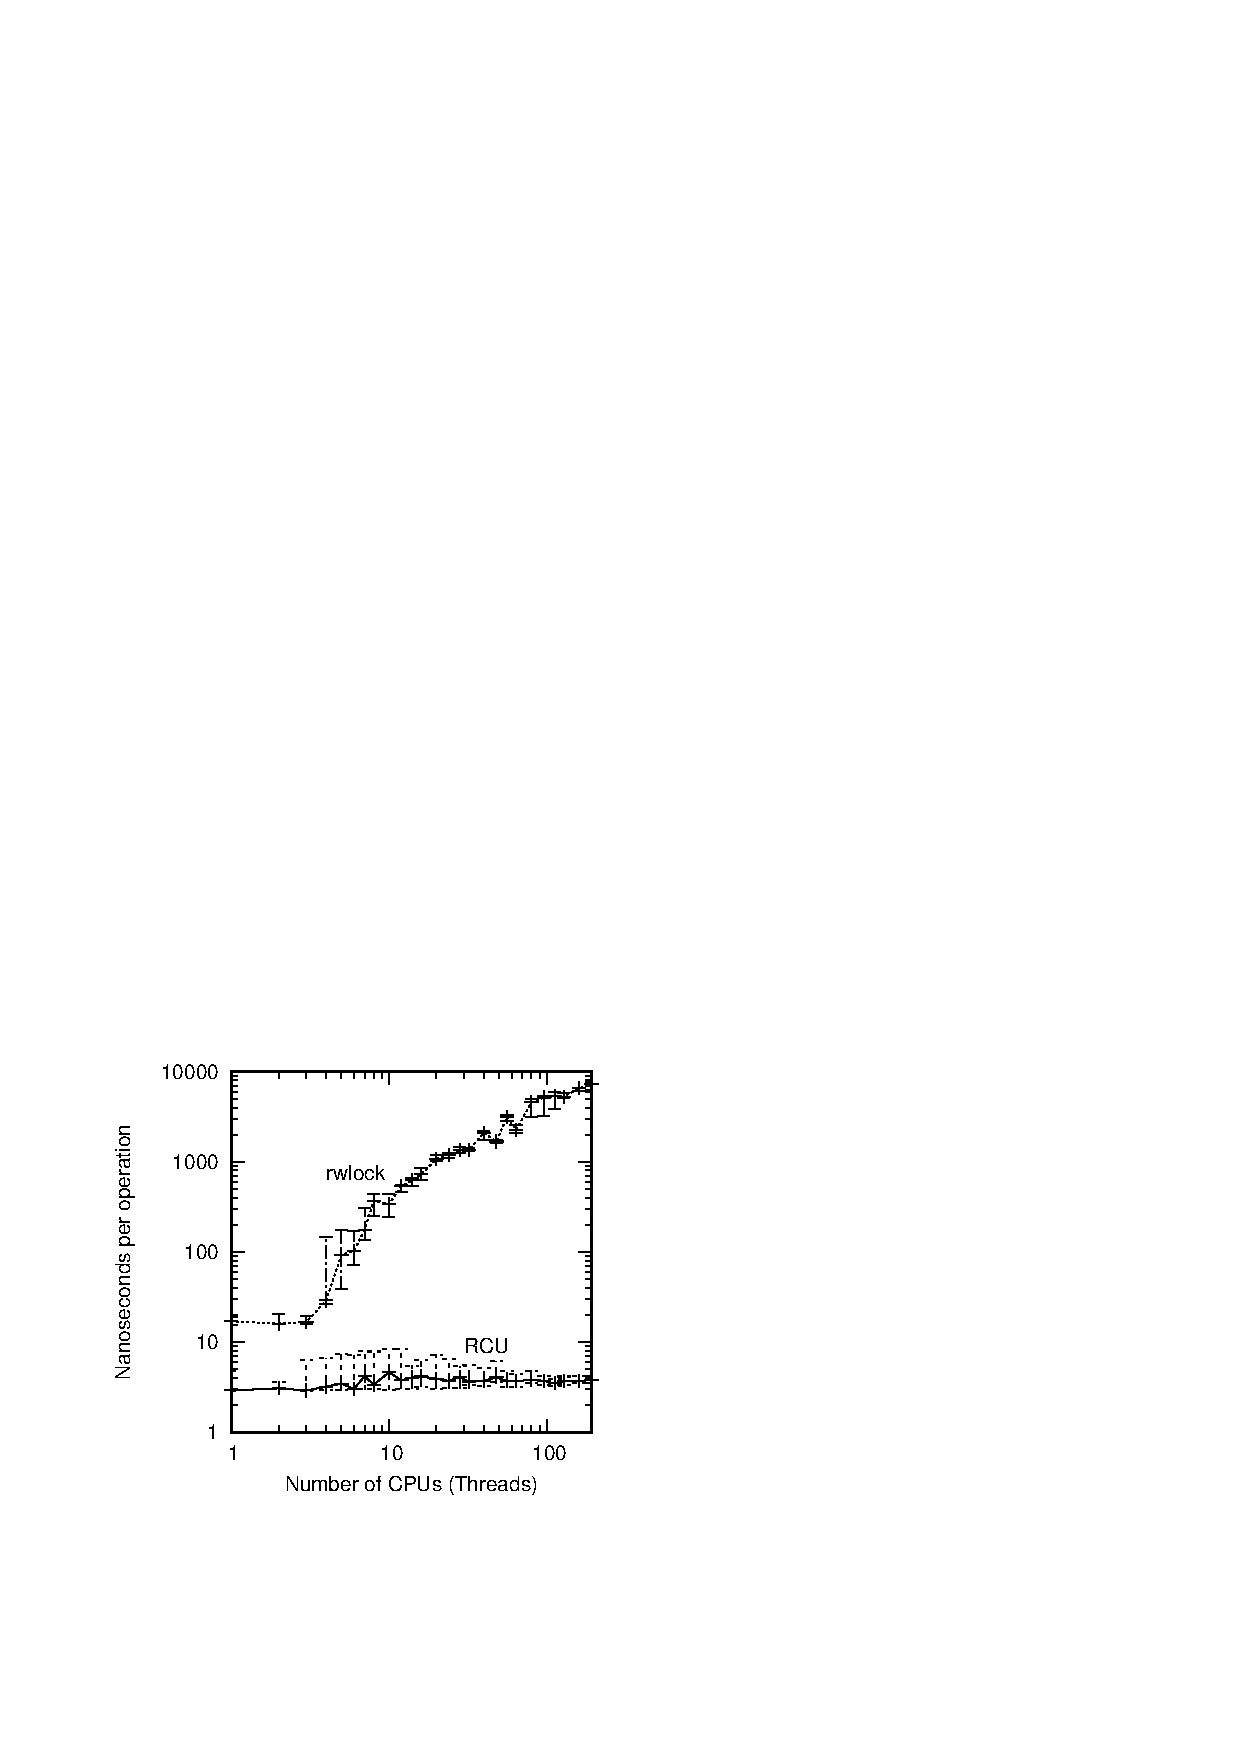
\includegraphics{defer/rwlockRCUperfPREEMPT}}
\caption{Performance Advantage of Preemptible RCU Over Reader-Writer Locking}
\label{fig:defer:Performance Advantage of Preemptible RCU Over Reader-Writer Locking}
\end{figure}

A more moderate view may be obtained from a \co{CONFIG_PREEMPT} kernel,
though RCU still beats reader-writer locking by between a factor of seven
on a single CPU and by three orders of magnitude on 192~CPUs, as shown in
\cref{fig:defer:Performance Advantage of Preemptible RCU Over Reader-Writer Locking},
which was generated on the same 448-CPU 2.10\,GHz x86 system.
Note the high variability of reader-writer locking at larger numbers of CPUs.
The error bars span the full range of data.

\QuickQuiz{
	Given that the system had no fewer than 448~hardware threads,
	why only 192~CPUs?
}\QuickQuizAnswer{
	Because the script (\path{rcuscale.sh}) that generates this data
	spawn a guest operating system for each set of points gathered,
	and on this particular system, both \co{qemu} and KVM limit the
	number of CPUs that may be configured into a given guest OS\@.
	Yes, it would have been possible to run a few more CPUs, but
	192 is a nice round number from a binary perspective, given
	that 256 is infeasible.
}\QuickQuizEnd

\begin{figure}
\centering
\resizebox{2.5in}{!}{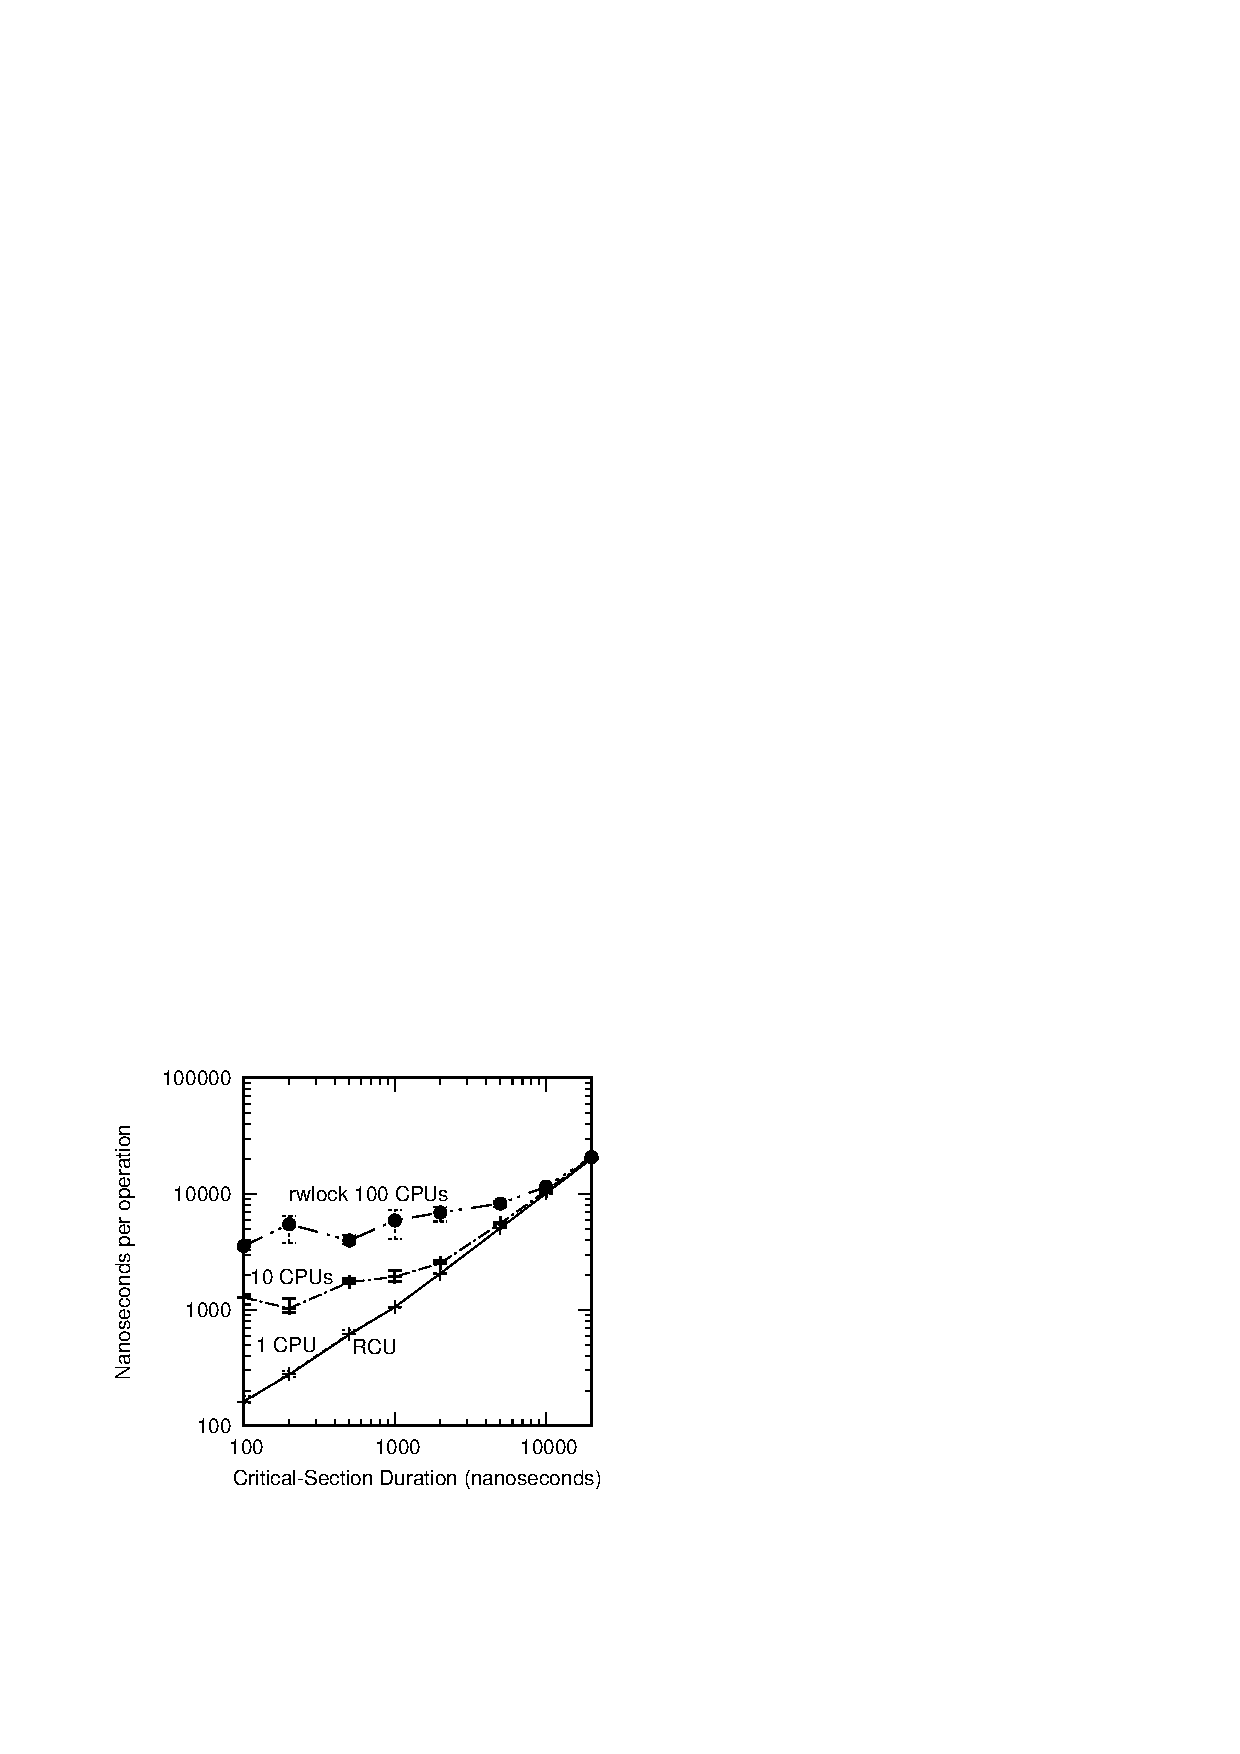
\includegraphics{defer/rwlockRCUperfwt}}
\caption{Comparison of RCU to Reader-Writer Locking as Function of Critical-Section Duration, 192 CPUs}
\label{fig:defer:Comparison of RCU to Reader-Writer Locking as Function of Critical-Section Duration}
\end{figure}

Of course, the low performance of reader-writer locking in
\cref{fig:defer:Performance Advantage of RCU Over Reader-Writer Locking,%
fig:defer:Performance Advantage of Preemptible RCU Over Reader-Writer Locking}
is exaggerated by the unrealistic zero-length critical sections.
The performance advantages of RCU decrease as the overhead of the critical
sections increase.
This decrease can be seen in
\cref{fig:defer:Comparison of RCU to Reader-Writer Locking as Function of Critical-Section Duration},
which was run on the same system as the previous plots.
Here, the y-axis represents the sum of the overhead of the read-side
primitives and that of the critical section and the x-axis represents
the critical-section overhead in nanoseconds.
But please note the logscale y~axis, which means that the small
separations between the traces still represent significant differences.
This figure shows non-preemptible RCU, but given that preemptible RCU's
read-side overhead is only about three nanoseconds, its plot would be
nearly identical to
\cref{fig:defer:Comparison of RCU to Reader-Writer Locking as Function of Critical-Section Duration}.

\QuickQuiz{
	Why the larger error ranges for the submicrosecond durations in
	\cref{fig:defer:Comparison of RCU to Reader-Writer Locking as Function of Critical-Section Duration}?
}\QuickQuizAnswer{
	Because smaller disturbances result in greater relative errors
	for smaller measurements.
	Also, the Linux kernel's \co{ndelay()} nanosecond-scale primitive
	is (as of 2020) less accurate than is the \co{udelay()} primitive
	used for the data for durations of a microsecond or more.
	It is instructive to compare to the zero-length case shown in
	\cref{fig:defer:Performance Advantage of RCU Over Reader-Writer Locking}.
}\QuickQuizEnd

There are three traces for reader-writer locking, with the upper trace
being for 100~CPUs, the next for 10~CPUs, and the lowest for 1~CPU\@.
So the greater the number of CPUs and the shorter the critical sections,
the greater is RCU's performance advantage.
These performance advantages are underscored by the fact that 100-CPU
systems are no longer uncommon and that a number of system calls (and
thus any RCU read-side critical sections that they contain) complete
within a microsecond.

In addition, as is discussed in the next section,
RCU read-side primitives are almost entirely deadlock-immune.


\paragraph{Deadlock Immunity}

Although RCU offers significant performance advantages for
read-mostly workloads, one of the primary reasons for creating
RCU in the first place was in fact its immunity to read-side
deadlocks.
This immunity stems from the fact that
RCU read-side primitives do not block, spin, or even
do backwards branches, so that their execution time is deterministic.
It is therefore impossible for them to participate in a deadlock
cycle.

\QuickQuiz{
	Is there an exception to this deadlock immunity, and if so,
	what sequence of events could lead to deadlock?
}\QuickQuizAnswer{
	One way to cause a deadlock cycle involving
	RCU read-side primitives is via the following (illegal) sequence
	of statements:

\begin{VerbatimU}
rcu_read_lock();
synchronize_rcu();
rcu_read_unlock();
\end{VerbatimU}

	The \co{synchronize_rcu()} cannot return until all
	pre-existing RCU read-side critical sections complete, but
	is enclosed in an RCU read-side critical section that cannot
	complete until the \co{synchronize_rcu()} returns.
	The result is a classic self-deadlock---you get the same
	effect when attempting to write-acquire a reader-writer lock
	while read-holding it.

	Note that this self-deadlock scenario does not apply to
	RCU QSBR, because the context switch performed by the
	\co{synchronize_rcu()} would act as a quiescent state
	for this CPU, allowing a grace period to complete.
	However, this is if anything even worse, because data used
	by the RCU read-side critical section might be freed as a
	result of the grace period completing.

	In short, do not invoke synchronous RCU update-side primitives
	from within an RCU read-side critical section.
}\QuickQuizEnd

An interesting consequence of RCU's read-side deadlock immunity is
that it is possible to unconditionally upgrade an RCU
reader to an RCU updater.
Attempting to do such an upgrade with reader-writer locking results
in deadlock.
A sample code fragment that does an RCU read-to-update upgrade follows:

\begin{VerbatimN}[samepage=true]
rcu_read_lock();
list_for_each_entry_rcu(p, &head, list_field) {
	do_something_with(p);
	if (need_update(p)) {
		spin_lock(my_lock);
		do_update(p);
		spin_unlock(&my_lock);
	}
}
rcu_read_unlock();
\end{VerbatimN}

Note that \co{do_update()} is executed under
the protection of the lock \emph{and} under RCU read-side protection.

Another interesting consequence of RCU's deadlock immunity is its
immunity to a large class of priority inversion problems.
For example, low-priority RCU readers cannot prevent a high-priority
RCU updater from acquiring the update-side lock.
Similarly, a low-priority RCU updater cannot prevent high-priority
RCU readers from entering an RCU read-side critical section.

\QuickQuiz{
	Immunity to both deadlock and priority inversion???
	Sounds too good to be true.
	Why should I believe that this is even possible?
}\QuickQuizAnswer{
	It really does work.
	After all, if it didn't work, the Linux kernel would not run.
}\QuickQuizEnd

\paragraph{Realtime Latency}

Because RCU read-side primitives neither spin nor block, they offer
excellent realtime latencies.
In addition, as noted earlier, this means that they are
immune to priority inversion
involving the RCU read-side primitives and locks.

However, RCU is susceptible to more subtle priority-inversion scenarios,
for example, a high-priority process blocked waiting for an RCU
grace period to elapse can be blocked by low-priority RCU readers
in \rt\ kernels.
This can be solved by using RCU priority
boosting~\cite{PaulEMcKenney2007BoostRCU,DinakarGuniguntala2008IBMSysJ}.

\paragraph{RCU Readers and Updaters Run Concurrently}

Because RCU readers never spin nor block, and because updaters are not
subject to any sort of rollback or abort semantics, RCU readers and
updaters must necessarily run concurrently.
This means that RCU readers might access stale data, and might even
see inconsistencies, either of which can render conversion from reader-writer
locking to RCU non-trivial.

\begin{figure}
\centering
\resizebox{3in}{!}{\includegraphics{defer/rwlockRCUupdate}}
\caption{Response Time of RCU vs.\@ Reader-Writer Locking}
\label{fig:defer:Response Time of RCU vs. Reader-Writer Locking}
\end{figure}

However, in a surprisingly large number of situations, inconsistencies and
stale data are not problems.
The classic example is the networking routing table.
Because routing updates can take considerable time to reach a given
system (seconds or even minutes), the system will have been sending
packets the wrong way for quite some time when the update arrives.
It is usually not a problem to continue sending updates the wrong
way for a few additional milliseconds.
Furthermore, because RCU updaters can make changes without waiting for
RCU readers to finish,
the RCU readers might well see the change more quickly than would
batch-fair
reader-writer-locking readers, as shown in
\cref{fig:defer:Response Time of RCU vs. Reader-Writer Locking}.

Once the update is received, the rwlock writer cannot proceed until the
last reader completes, and subsequent readers cannot proceed until the
writer completes.
However, these subsequent readers are guaranteed to see the new value,
as indicated by the green shading of the rightmost boxes.
In contrast, RCU readers and updaters do not block each other, which permits
the RCU readers to see the updated values sooner.
Of course, because their execution overlaps that of the RCU updater,
\emph{all} of the RCU readers might well see updated values, including
the three readers that started before the update.
Nevertheless only the green-shaded rightmost RCU readers
are \emph{guaranteed} to see the updated values.

Reader-writer locking and RCU simply provide different guarantees.
With reader-writer locking, any reader that begins after the writer begins
is guaranteed to see new values, and any reader that attempts to
begin while the writer is spinning might or might not see new values,
depending on the reader/writer preference of the rwlock implementation in
question.
In contrast, with RCU, any reader that begins after the updater completes
is guaranteed to see new values, and any reader that completes after the
updater begins might or might not see new values, depending on timing.

The key point here is that, although reader-writer locking does
indeed guarantee consistency within the confines of the computer system,
there are situations where this consistency comes at the price of
increased \emph{inconsistency} with the outside world.
In other words, reader-writer locking obtains internal consistency at the
price of silently stale data with respect to the outside world.

Nevertheless, there are situations where inconsistency and stale
data within the confines of the system cannot be tolerated.
Fortunately,
there are a number of approaches that avoid inconsistency and stale
data~\cite{PaulEdwardMcKenneyPhD,Arcangeli03}, and some
methods based on reference counting are discussed in
\cref{sec:defer:Reference Counting}.

\paragraph{Low-Priority RCU Readers Can Block High-Priority Reclaimers}

In Realtime RCU~\cite{DinakarGuniguntala2008IBMSysJ} or
SRCU~\cite{PaulEMcKenney2006c},
a preempted reader will prevent a grace period from completing, even if
a high-priority task is blocked waiting for that grace period to complete.
Realtime RCU can avoid this problem by substituting \co{call_rcu()}
for \co{synchronize_rcu()} or by using RCU priority
boosting~\cite{PaulEMcKenney2007BoostRCU,DinakarGuniguntala2008IBMSysJ},
which is still in experimental status as of early 2008.
It might become necessary to augment SRCU and QRCU with priority boosting,
but not before a clear real-world need is demonstrated.

\paragraph{RCU Grace Periods Extend for Many Milliseconds}

With the exception of userspace
RCU~\cite{MathieuDesnoyers2009URCU,PaulMcKenney2013LWNURCU},
expedited grace periods, and several of the ``toy''
RCU implementations described in
\cref{chp:app:``Toy'' RCU Implementations},
RCU grace periods extend milliseconds.
Although there are a number of techniques to render such long delays
harmless, including use of the asynchronous interfaces where available
(\co{call_rcu()} and \co{call_rcu_bh()}), this situation
is a major reason for the rule of thumb that RCU be used in read-mostly
situations.

\paragraph{Code: Reader-Writer Locking vs.\@ RCU Code}

In the best case, the conversion from reader-writer locking to RCU
is quite simple, as shown in
\cref{lst:defer:Converting Reader-Writer Locking to RCU: Data,%
lst:defer:Converting Reader-Writer Locking to RCU: Search,%
lst:defer:Converting Reader-Writer Locking to RCU: Deletion},
all taken from
Wikipedia~\cite{WikipediaRCU}.

\begin{listing*}
{ \scriptsize
\begin{verbbox}
 1 struct el {                           1 struct el {
 2   struct list_head lp;                2   struct list_head lp;
 3   long key;                           3   long key;
 4   spinlock_t mutex;                   4   spinlock_t mutex;
 5   int data;                           5   int data;
 6   /* Other data fields */             6   /* Other data fields */
 7 };                                    7 };
 8 DEFINE_RWLOCK(listmutex);             8 DEFINE_SPINLOCK(listmutex);
 9 LIST_HEAD(head);                      9 LIST_HEAD(head);
\end{verbbox}
}
\hspace*{0.9in}\OneColumnHSpace{-0.5in}
\IfEbookSize{\hspace*{-1.05in}}{}\theverbbox
\caption{Converting Reader-Writer Locking to RCU: Data}
\label{lst:defer:Converting Reader-Writer Locking to RCU: Data}
\end{listing*}

\begin{listing*}
{ \scriptsize
\begin{verbbox}
 1 int search(long key, int *result)     1 int search(long key, int *result)
 2 {                                     2 {
 3   struct el *p;                       3   struct el *p;
 4                                       4
 5   read_lock(&listmutex);              5   rcu_read_lock();
 6   list_for_each_entry(p, &head, lp) { 6   list_for_each_entry_rcu(p, &head, lp) {
 7     if (p->key == key) {              7     if (p->key == key) {
 8       *result = p->data;              8       *result = p->data;
 9       read_unlock(&listmutex);        9       rcu_read_unlock();
10       return 1;                      10       return 1;
11     }                                11     }
12   }                                  12   }
13   read_unlock(&listmutex);           13   rcu_read_unlock();
14   return 0;                          14   return 0;
15 }                                    15 }
\end{verbbox}
}
\hspace*{0.9in}\OneColumnHSpace{-0.5in}
\IfEbookSize{\hspace*{-1.05in}}{}\theverbbox
\caption{Converting Reader-Writer Locking to RCU: Search}
\label{lst:defer:Converting Reader-Writer Locking to RCU: Search}
\end{listing*}

\begin{listing*}
{ \scriptsize
\begin{verbbox}
 1 int delete(long key)                  1 int delete(long key)
 2 {                                     2 {
 3   struct el *p;                       3   struct el *p;
 4                                       4
 5   write_lock(&listmutex);             5   spin_lock(&listmutex);
 6   list_for_each_entry(p, &head, lp) { 6   list_for_each_entry(p, &head, lp) {
 7     if (p->key == key) {              7     if (p->key == key) {
 8       list_del(&p->lp);               8       list_del_rcu(&p->lp);
 9       write_unlock(&listmutex);       9       spin_unlock(&listmutex);
                                        10       synchronize_rcu();
10       kfree(p);                      11       kfree(p);
11       return 1;                      12       return 1;
12     }                                13     }
13   }                                  14   }
14   write_unlock(&listmutex);          15   spin_unlock(&listmutex);
15   return 0;                          16   return 0;
16 }                                    17 }
\end{verbbox}
}
\hspace*{0.9in}\OneColumnHSpace{-0.5in}
\IfEbookSize{\hspace*{-1.05in}}{}\theverbbox
\caption{Converting Reader-Writer Locking to RCU: Deletion}
\label{lst:defer:Converting Reader-Writer Locking to RCU: Deletion}
\end{listing*}

However, the transformation is not always this straightforward.
This is because neither the \co{spin_lock()} nor the
\co{synchronize_rcu()} in
\cref{lst:defer:Converting Reader-Writer Locking to RCU: Deletion}
exclude the readers in
\cref{lst:defer:Converting Reader-Writer Locking to RCU: Search}.
First, the \co{spin_lock()} does not interact in any way with
\co{rcu_read_lock()} and \co{rcu_read_unlock()}, thus not excluding them.
Second, although both \co{write_lock()} and \co{synchronize_rcu()}
wait for pre-existing readers, only \co{write_lock()} prevents
subsequent readers from commencing.\footnote{
	Kudos to whoever pointed this out to Paul.}
Thus, \co{synchronize_rcu()} cannot exclude readers.
It is therefore surprising that a great many situations
using reader-writer locking can be easily converted to RCU\@.

More-elaborate cases of replacing reader-writer locking with RCU
may be found
elsewhere~\cite{NeilBrown2015PathnameLookup,NeilBrown2015RCUwalk}.

\paragraph{Semantics: Reader-Writer Locking vs.\@ RCU Semantics}

Reader-writer locking semantics can be roughly and informally summarized
by the following three temporal constraints:

\begin{enumerate}
\item	Write-side acquisitions wait for any read-holders to release
	the lock.
\item	Writer-side acquisitions wait for any write-holder to release
	the lock.
\item	Read-side acquisitions wait for any write-holder to release
	the lock.
\end{enumerate}

RCU dispenses entirely with constraint~\#3 and weakens the other two
as follows:

\begin{enumerate}
\item	Writers wait for any pre-existing read-holders before progressing
	to the destructive phase of their update (usually the freeing of
	memory).
\item	Writers synchronize with each other as needed.
\end{enumerate}

It is of course this weakening that permits RCU implementations to attain
excellent performance and scalability.
RCU use cases compensate for this weakening in a surprisingly large number
of ways, but most commonly by imposing spatial constraints:

\begin{enumerate}
\item	New data is placed in newly allocated memory.
\item	Old data is freed, but only after:
	\begin{enumerate}
	\item	That data has been unlinked so as to be inaccessible
		to later readers, and
	\item	A subsequent RCU grace period has elapsed.
	\end{enumerate}
\end{enumerate}

In short, RCU attains its read-side performance and scalability by
constructing semantics based on combined temporal and spatial constraints.

\subsubsection{RCU is a Restricted Reference-Counting Mechanism}
\label{sec:defer:RCU is a Restricted Reference-Counting Mechanism}

Because grace periods are not allowed to complete while
there is an RCU read-side critical section in progress,
the RCU read-side primitives may be used as a restricted
reference-counting mechanism.
For example, consider the following code fragment:

\begin{VerbatimN}
rcu_read_lock();  /* acquire reference. */
p = rcu_dereference(head);
/* do something with p. */
rcu_read_unlock();  /* release reference. */
\end{VerbatimN}

The \co{rcu_read_lock()} primitive can be thought of as
acquiring a reference to \co{p}, because a grace period
starting after the \co{rcu_dereference()} assigns to \co{p}
cannot possibly end until after we reach the matching
\co{rcu_read_unlock()}.
This reference-counting scheme is restricted in that
we are not allowed to block in RCU read-side critical sections,
nor are we permitted to hand off an RCU read-side critical section
from one task to another.

Regardless of these restrictions,
the following code can safely delete \co{p}:

\begin{VerbatimN}
spin_lock(&mylock);
p = head;
rcu_assign_pointer(head, NULL);
spin_unlock(&mylock);
/* Wait for all references to be released. */
synchronize_rcu();
kfree(p);
\end{VerbatimN}

The assignment to \co{head} prevents any future references
to \co{p} from being acquired, and the \co{synchronize_rcu()}
waits for any previously acquired references to be released.

\QuickQuiz{
	But wait!
	This is exactly the same code that might be used when thinking
	of RCU as a replacement for reader-writer locking!
	What gives?
}\QuickQuizAnswer{
	This is an effect of the Law of Toy Examples:
	beyond a certain point, the code fragments look the same.
	The only difference is in how we think about the code.
	However, this difference can be extremely important.
	For but one example of the importance, consider that if we think
	of RCU as a restricted reference counting scheme, we would never
	be fooled into thinking that the updates would exclude the RCU
	read-side critical sections.

	It nevertheless is often useful to think of RCU as a replacement
	for reader-writer locking, for example, when you are replacing
	reader-writer locking with RCU\@.
}\QuickQuizEnd

Of course, RCU can also be combined with traditional reference counting,
as discussed in
\cref{sec:together:Refurbish Reference Counting}.

\begin{figure}
\centering
\resizebox{2.5in}{!}{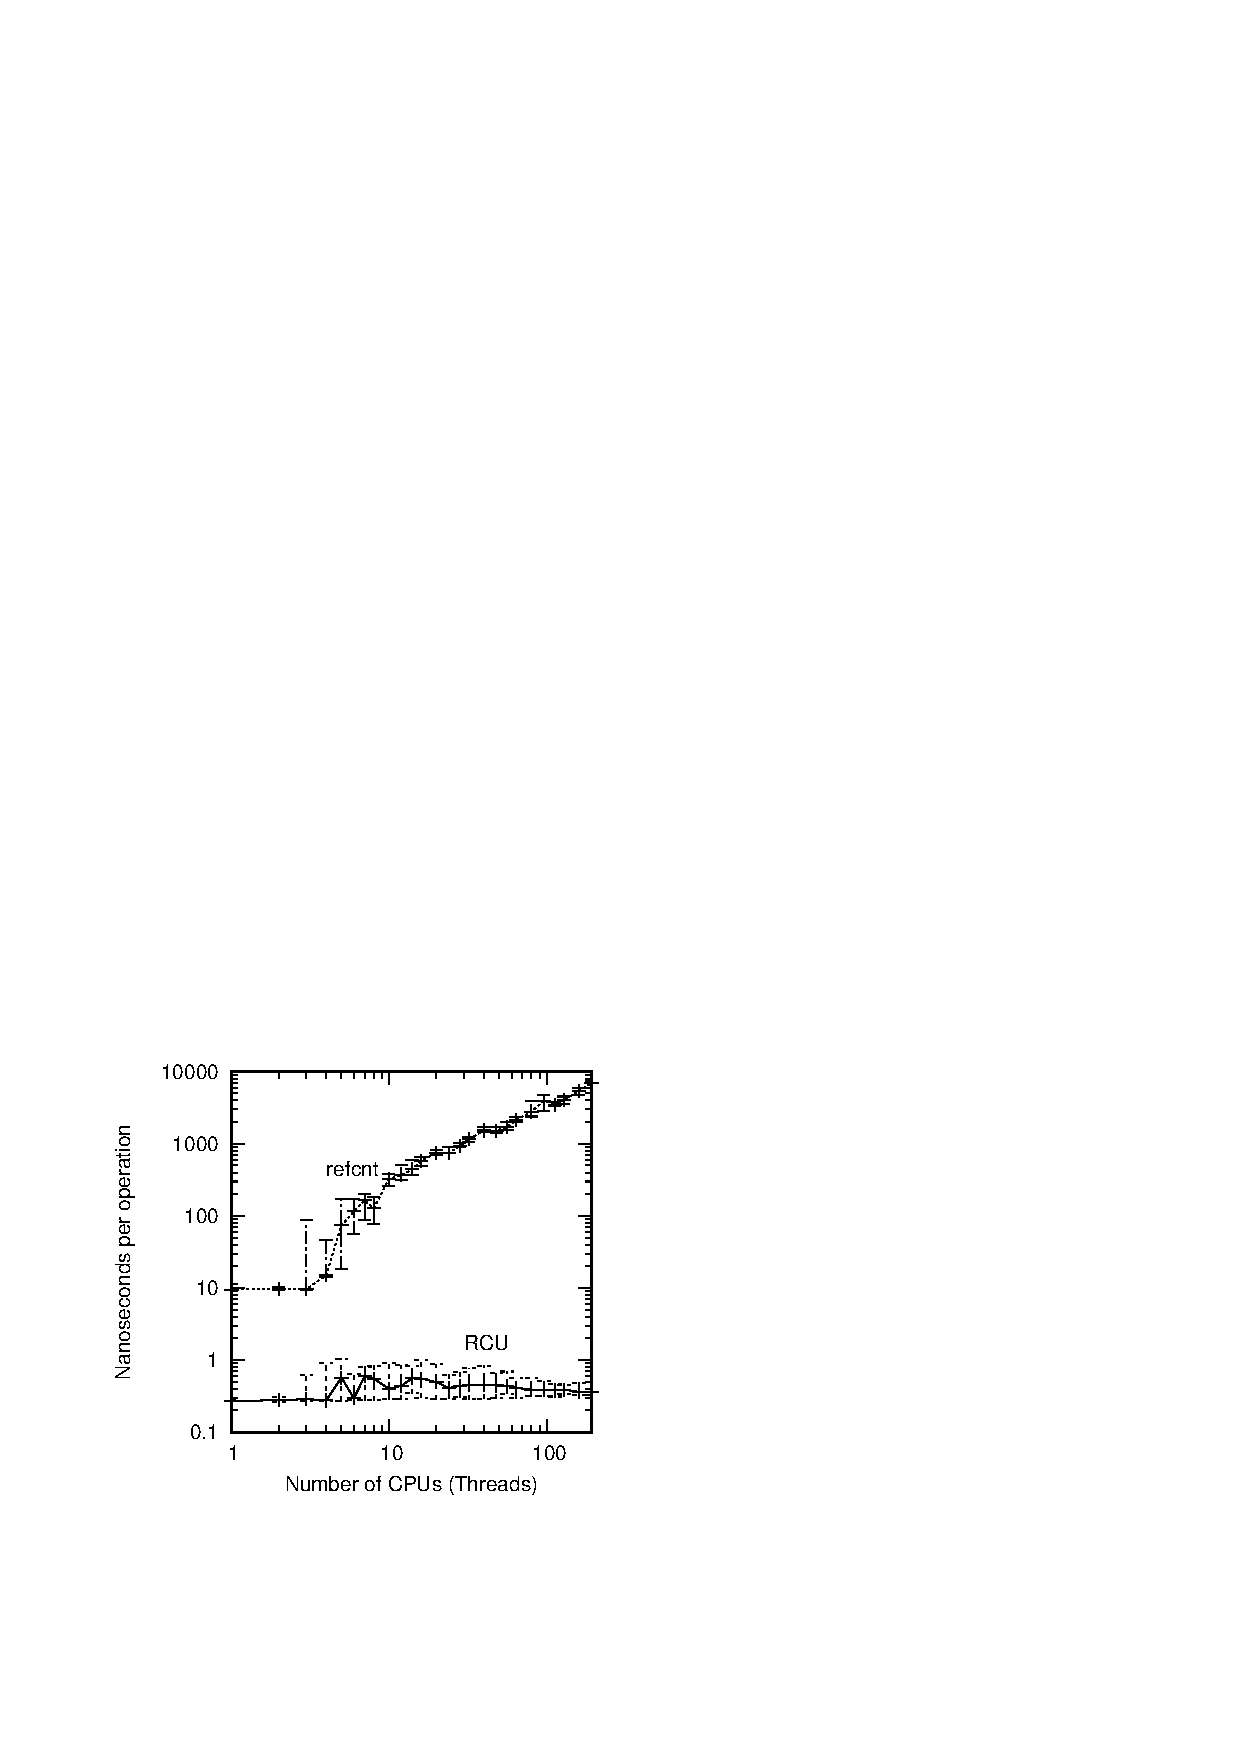
\includegraphics{defer/refcntRCUperf}}
\caption{Performance of RCU vs.\@ Reference Counting}
\label{fig:defer:Performance of RCU vs. Reference Counting}
\end{figure}

\begin{figure}
\centering
\resizebox{2.5in}{!}{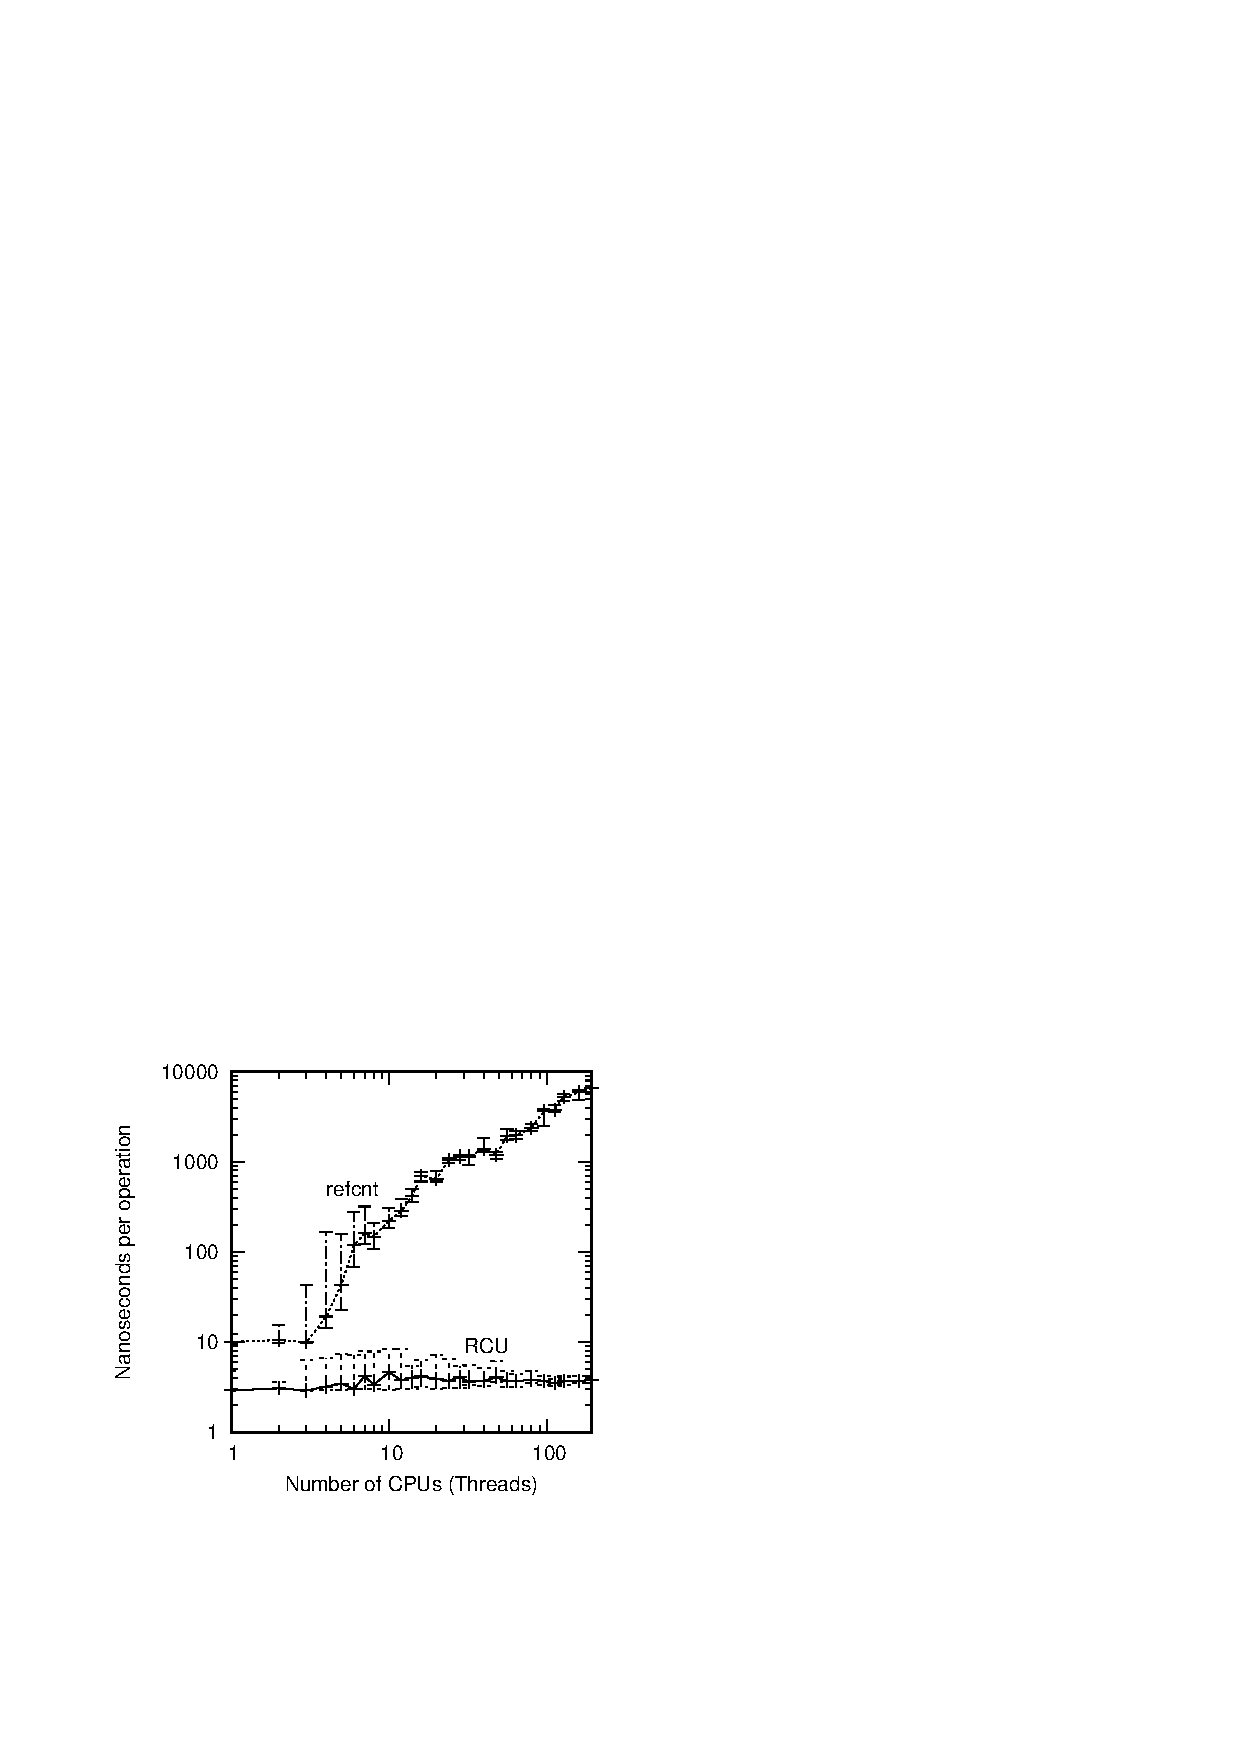
\includegraphics{defer/refRCUperfPREEMPT}}
\caption{Performance of Preemptible RCU vs.\@ Reference Counting}
\label{fig:defer:Performance of Preemptible RCU vs. Reference Counting}
\end{figure}

But why bother?
Again, part of the answer is performance, as shown in
\cref{fig:defer:Performance of RCU vs. Reference Counting,%
fig:defer:Performance of Preemptible RCU vs. Reference Counting},
again showing data taken on a 448-CPU 2.1\,GHz Intel x86 system
for non-preemptible and preemptible Linux-kernel RCU, respectively.
Non-preemptible RCU's advantage over reference counting ranges from
more than an order of magnitude at one CPU up to about four orders of
magnitude at 192~CPUs.
Preemptible RCU's advantage ranges from about a factor of three at
one CPU up to about three orders of magnitude at 192~CPUs.

\begin{figure}
\centering
\resizebox{2.5in}{!}{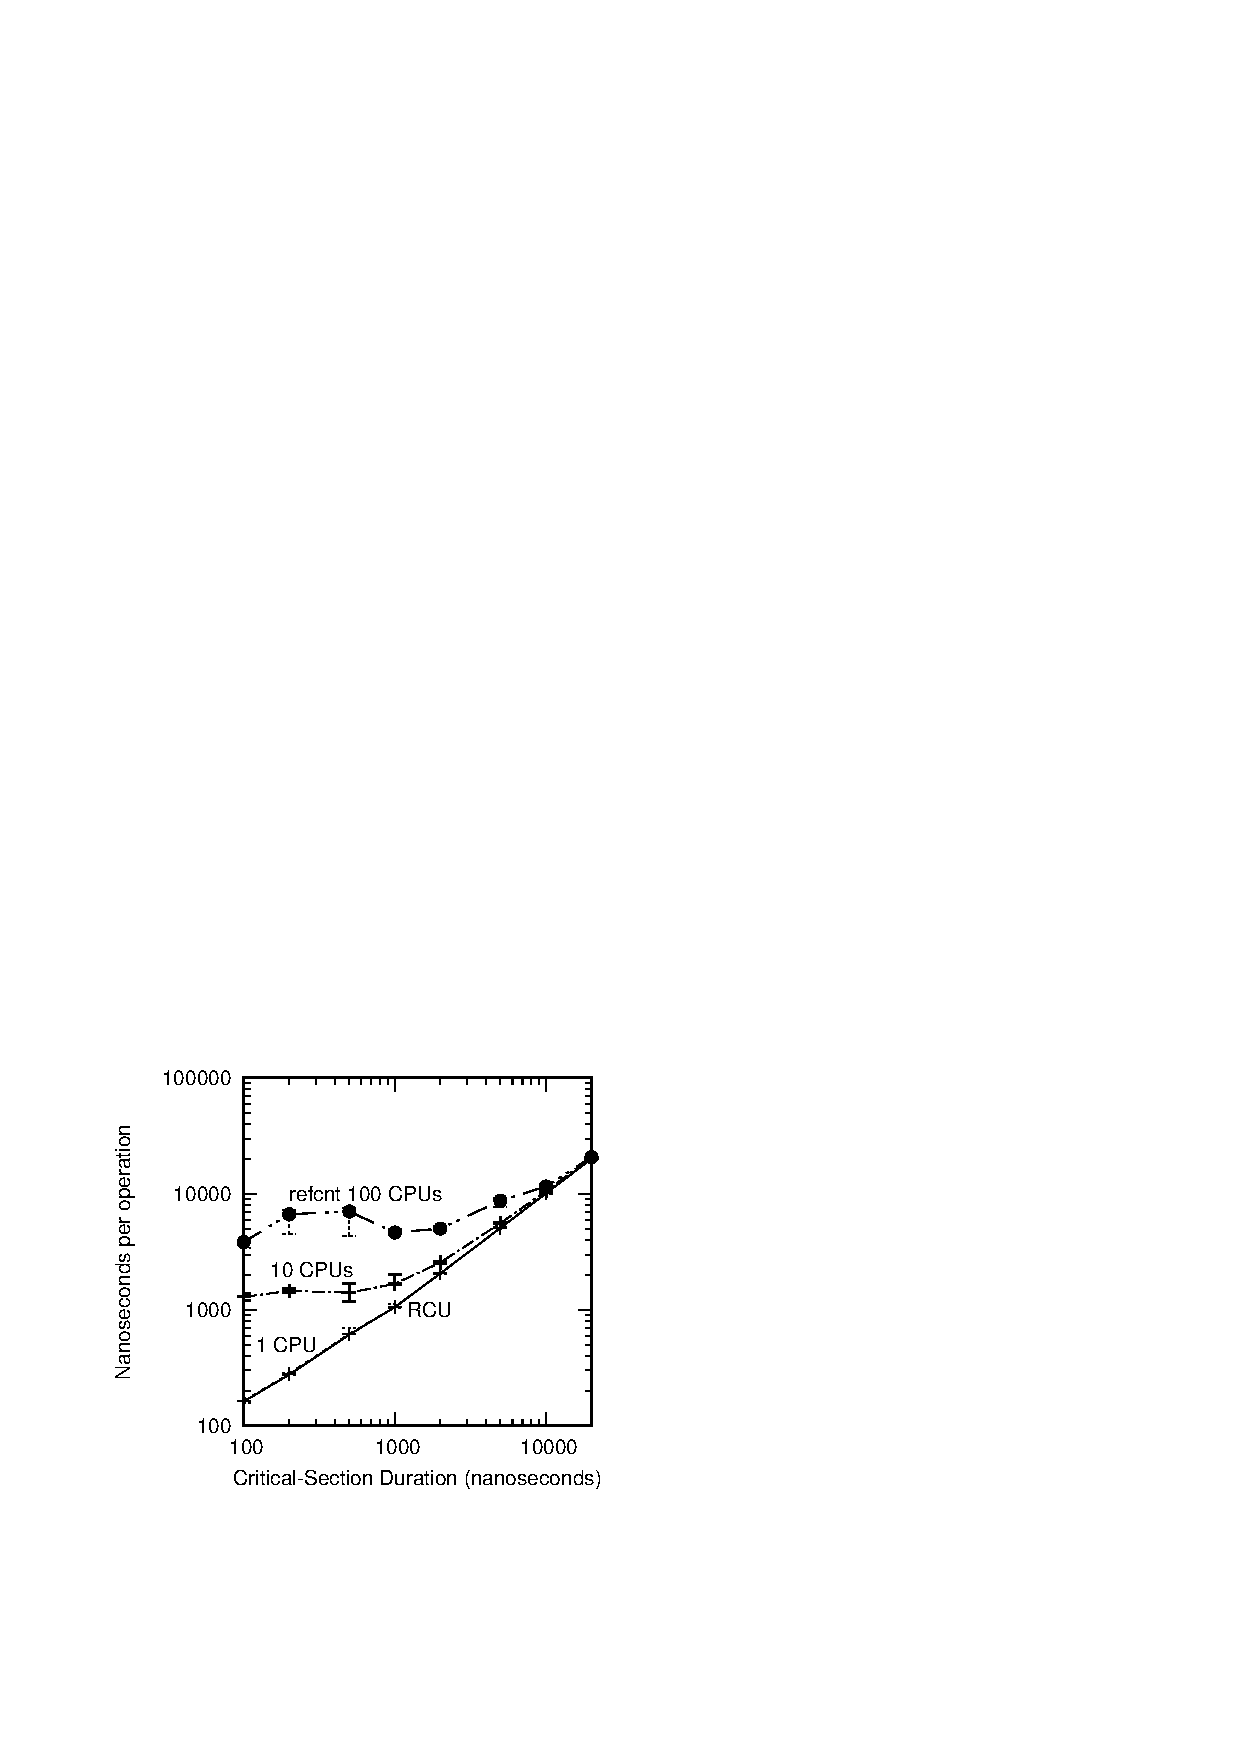
\includegraphics{defer/refRCUperfwt}}
\caption{Response Time of RCU vs.\@ Reference Counting, 192 CPUs}
\label{fig:defer:Response Time of RCU vs. Reference Counting}
\end{figure}

However, as with reader-writer locking, the performance advantages of
RCU are most pronounced for short-duration critical sections and for
large numbers of CPUs, as shown in
\cref{fig:defer:Response Time of RCU vs. Reference Counting}
for the same system.
In addition, as with reader-writer locking, many system calls (and thus
any RCU read-side critical sections that they contain) complete in
a few microseconds.

However, the restrictions that go with RCU can be quite onerous.
For example, in many cases, the prohibition against sleeping while in an RCU
read-side critical section would defeat the entire purpose.
The next section looks at ways of addressing this problem, while also
reducing the complexity of traditional reference counting, at least in
some cases.\footnote{
	Other cases might be better served by the hazard pointers
	mechanism described in \cref{sec:defer:Hazard Pointers}.}

\subsubsection{RCU is a Bulk Reference-Counting Mechanism}
\label{sec:defer:RCU is a Bulk Reference-Counting Mechanism}

As noted in the preceding section,
traditional reference counters are usually associated with a specific
data structure, or perhaps a specific group of data structures.
However, maintaining a single global reference counter for a large
variety of data structures typically results in bouncing
the cache line containing the reference count.
Such cache-line bouncing can severely degrade performance.

In contrast, RCU's lightweight read-side primitives permit
extremely frequent read-side usage with negligible performance
degradation, permitting RCU to be used as a ``bulk reference-counting''
mechanism with little or no performance penalty.
Situations where a reference must be held by a single task across a
section of code that blocks may be accommodated with
Sleepable RCU (SRCU)~\cite{PaulEMcKenney2006c}.
This fails to cover the not-uncommon situation where a reference is ``passed''
from one task to another, for example, when a reference is acquired
when starting an I/O and released in the corresponding completion
interrupt handler.
(In principle, this could be handled by the SRCU implementation,
but in practice, it is not yet clear whether this is a good tradeoff.)

Of course, SRCU brings restrictions of its own, namely that the
return value from \co{srcu_read_lock()} be passed into the
corresponding \co{srcu_read_unlock()}, and that no SRCU primitives
be invoked from hardware interrupt handlers or from \IXacrf{nmi}
handlers.
The jury is still out as to how much of a problem is presented by
these restrictions, and as to how they can best be handled.

\subsubsection{RCU is a Poor Man's Garbage Collector}
\label{sec:defer:RCU is a Poor Man's Garbage Collector}

A not-uncommon exclamation made by people first learning about
RCU is ``RCU is sort of like a garbage collector!''
This exclamation has a large grain of truth, but it can also be
misleading.

Perhaps the best way to think of the relationship between RCU
and automatic garbage collectors (GCs) is that RCU resembles
a GC in that the \emph{timing} of collection is automatically
determined, but that RCU differs from a GC in that: (1)~the programmer
must manually indicate when a given data structure is eligible
to be collected, and (2)~the programmer must manually mark the
RCU read-side critical sections where references might be held.

Despite these differences, the resemblance does go quite deep.
In fact, the first RCU-like mechanism I am aware of used a
reference-count-based garbage collector to handle the grace
periods~\cite{Kung80}, and the connection between RCU and
garbage collection has been noted more
recently~\cite{HarshalSheth2016goRCU}.
Nevertheless, a better way of thinking of RCU is described in the
following section.

\subsubsection{RCU is an MVCC}
\label{sec:defer:RCU is an MVCC}

RCU can also be thought of as a simplified multi-version concurrency
control (MVCC) mechanism with weak consistency criteria.
The multi-version aspects were touched upon in
\cref{sec:defer:Maintain Multiple Versions of Recently Updated Objects}.
However, in its native form, RCU provides version consistency only
within a given RCU-protected data element.

However, a number of techniques can be used to restore version consistency
at a higher level, for example, using sequence locking
(see \cref{sec:together:Correlated Data Elements})
or imposing additional levels of indirection
(see \cref{sec:together:Correlated Fields}).

\subsubsection{RCU Provides Existence Guarantees}
\label{sec:defer:RCU Provides Existence Guarantees}

Gamsa et al.~\cite{Gamsa99}
discuss existence guarantees and describe how a mechanism
resembling RCU can be used to provide these existence guarantees
(see Section~5 on page 7 of the PDF), and
\cref{sec:locking:Lock-Based Existence Guarantees}
discusses how to guarantee existence via locking, along with the
ensuing disadvantages of doing so.
The effect is that if any RCU-protected data element is accessed
within an RCU read-side critical section, that data element is
guaranteed to remain in existence for the duration of that RCU
read-side critical section.

\begin{listing}
\begin{fcvlabel}[ln:defer:Existence Guarantees Enable Per-Element Locking]
\begin{VerbatimL}[commandchars=\\\@\$]
int delete(int key)
{
	struct element *p;
	int b;

	b = hashfunction(key);			\lnlbl@hash$
	rcu_read_lock();			\lnlbl@rdlock$
	p = rcu_dereference(hashtable[b]);
	if (p == NULL || p->key != key) {	\lnlbl@chkkey$
		rcu_read_unlock();		\lnlbl@rdunlock1$
		return 0;			\lnlbl@ret_0:a$
	}
	spin_lock(&p->lock);			\lnlbl@acq$
	if (hashtable[b] == p && p->key == key) {\lnlbl@chkkey2$
		rcu_read_unlock();		\lnlbl@rdunlock2$
		rcu_assign_pointer(hashtable[b], NULL);\lnlbl@remove$
		spin_unlock(&p->lock);		\lnlbl@rel1$
		synchronize_rcu();		\lnlbl@sync_rcu$
		kfree(p);			\lnlbl@kfree$
		return 1;			\lnlbl@ret_1$
	}
	spin_unlock(&p->lock);			\lnlbl@rel2$
	rcu_read_unlock();			\lnlbl@rdunlock3$
	return 0;				\lnlbl@ret_0:b$
}
\end{VerbatimL}
\end{fcvlabel}
\caption{Existence Guarantees Enable Per-Element Locking}
\label{lst:defer:Existence Guarantees Enable Per-Element Locking}
\end{listing}

\begin{fcvref}[ln:defer:Existence Guarantees Enable Per-Element Locking]
\Cref{lst:defer:Existence Guarantees Enable Per-Element Locking}
demonstrates how RCU-based existence guarantees can enable
per-element locking via a function that deletes an element from
a hash table.
\Clnref{hash} computes a hash function, and \clnref{rdlock} enters an RCU
read-side critical section.
If \clnref{chkkey} finds that the corresponding bucket of the hash table is
empty or that the element present is not the one we wish to delete,
then \clnref{rdunlock1} exits the RCU read-side critical section and
\clnref{ret_0:a}
indicates failure.
\end{fcvref}

\QuickQuiz{
	What if the element we need to delete is not the first element
	of the list on
	\clnrefr{ln:defer:Existence Guarantees Enable Per-Element Locking:chkkey} of
	\cref{lst:defer:Existence Guarantees Enable Per-Element Locking}?
}\QuickQuizAnswer{
	As with
	\cref{lst:locking:Per-Element Locking Without Existence Guarantees},
	this is a very simple hash table with no chaining, so the only
	element in a given bucket is the first element.
	The reader is again invited to adapt this example to a hash table with
	full chaining.
	Less energetic reader might wish to refer to
	\cref{chp:Data Structures}.
}\QuickQuizEnd

\begin{fcvref}[ln:defer:Existence Guarantees Enable Per-Element Locking]
Otherwise, \clnref{acq} acquires the update-side spinlock, and
\clnref{chkkey2} then checks that the element is still the one that we want.
If so, \clnref{rdunlock2} leaves the RCU read-side critical section,
\clnref{remove} removes it from the table, \clnref{rel1} releases
the lock, \clnref{sync_rcu} waits for all pre-existing RCU read-side critical
sections to complete, \clnref{kfree} frees the newly removed element,
and \clnref{ret_1} indicates success.
If the element is no longer the one we want, \clnref{rel2} releases
the lock, \clnref{rdunlock3} leaves the RCU read-side critical section,
and \clnref{ret_0:b} indicates failure to delete the specified key.
\end{fcvref}

\QuickQuizSeries{%
\QuickQuizB{
	\begin{fcvref}[ln:defer:Existence Guarantees Enable Per-Element Locking]
	Why is it OK to exit the RCU read-side critical section on
	\clnref{rdunlock2} of
	\cref{lst:defer:Existence Guarantees Enable Per-Element Locking}
	before releasing the lock on \clnref{rel1}?
	\end{fcvref}
}\QuickQuizAnswerB{
	\begin{fcvref}[ln:defer:Existence Guarantees Enable Per-Element Locking]
	First, please note that the second check on \clnref{chkkey2} is
	necessary because some other
	CPU might have removed this element while we were waiting
	to acquire the lock.
	However, the fact that we were in an RCU read-side critical section
	while acquiring the lock guarantees that this element could not
	possibly have been re-allocated and re-inserted into this
	hash table.
	Furthermore, once we acquire the lock, the lock itself guarantees
	the element's existence, so we no longer need to be in an
	RCU read-side critical section.

	The question as to whether it is necessary to re-check the
	element's key is left as an exercise to the reader.
	% A re-check is necessary if the key can mutate or if it is
	% necessary to reject deleted entries (in cases where deletion
	% is recorded by mutating the key.
	\end{fcvref}
}\QuickQuizEndB
%
\QuickQuizE{
	\begin{fcvref}[ln:defer:Existence Guarantees Enable Per-Element Locking]
	Why not exit the RCU read-side critical section on
	\clnref{rdunlock3} of
	\cref{lst:defer:Existence Guarantees Enable Per-Element Locking}
	before releasing the lock on \clnref{rel2}?
	\end{fcvref}
}\QuickQuizAnswerE{
	Suppose we reverse the order of these two lines.
	Then this code is vulnerable to the following sequence of
	events:
	\begin{enumerate}
	\begin{fcvref}[ln:defer:Existence Guarantees Enable Per-Element Locking]
	\item	CPU~0 invokes \co{delete()}, and finds the element
		to be deleted, executing through \clnref{rdunlock2}.
		It has not yet actually deleted the element, but
		is about to do so.
	\item	CPU~1 concurrently invokes \co{delete()}, attempting
		to delete this same element.
		However, CPU~0 still holds the lock, so CPU~1 waits
		for it at \clnref{acq}.
	\item	CPU~0 executes \clnref{remove,rel1},
		and blocks at \clnref{sync_rcu} waiting for CPU~1
		to exit its RCU read-side critical section.
	\item	CPU~1 now acquires the lock, but the test on \clnref{chkkey2}
		fails because CPU~0 has already removed the element.
		CPU~1 now executes \clnref{rel2}
                (which we switched with \clnref{rdunlock3}
		for the purposes of this Quick Quiz)
		and exits its RCU read-side critical section.
	\item	CPU~0 can now return from \co{synchronize_rcu()},
		and thus executes \clnref{kfree}, sending the element to
		the freelist.
	\item	CPU~1 now attempts to release a lock for an element
		that has been freed, and, worse yet, possibly
		reallocated as some other type of data structure.
		This is a fatal memory-corruption error.
	\end{fcvref}
	\end{enumerate}
}\QuickQuizEndE
}

Alert readers will recognize this as only a slight variation on
the original ``RCU is a way of waiting for things to finish'' theme,
which is addressed in
\cref{sec:defer:RCU is a Way of Waiting for Things to Finish}.
They might also note the deadlock-immunity advantages over the lock-based
existence guarantees discussed in
\cref{sec:locking:Lock-Based Existence Guarantees}.

\subsubsection{RCU Provides Type-Safe Memory}
\label{sec:defer:RCU Provides Type-Safe Memory}

A number of lockless algorithms do not require that a given data
element keep the same identity through a given RCU read-side critical
section referencing it---but only if that data element retains the
same type.
In other words, these lockless algorithms can tolerate a given data
element being freed and reallocated as the same type of structure
while they are referencing it, but must prohibit a change in type.
This guarantee, called ``type-safe memory'' in
academic literature~\cite{Cheriton96a},
is weaker than the existence guarantees in the
previous section, and is therefore quite a bit harder to work with.
Type-safe memory algorithms in the Linux kernel make use of slab caches,
specially marking these caches with \co{SLAB_TYPESAFE_BY_RCU}
so that RCU is used when returning a freed-up
slab to system memory.
This use of RCU guarantees that any in-use element of
such a slab will remain in that slab, thus retaining its type,
for the duration of any pre-existing RCU read-side critical sections.

\QuickQuiz{
	But what if there is an arbitrarily long series of RCU
	read-side critical sections in multiple threads, so that at
	any point in time there is at least one thread in the system
	executing in an RCU read-side critical section?
	Wouldn't that prevent any data from a \co{SLAB_TYPESAFE_BY_RCU}
	slab ever being returned to the system, possibly resulting
	in OOM events?
}\QuickQuizAnswer{
	There could certainly be an arbitrarily long period of time
	during which at least one thread is always in an RCU read-side
	critical section.
	However, the key words in the description in
	\cref{sec:defer:RCU Provides Type-Safe Memory}
	are ``in-use'' and ``pre-existing''.
	Keep in mind that a given RCU read-side critical section is
	conceptually only permitted to gain references to data elements
	that were in use at the beginning of that critical section.
	Furthermore, remember that a slab cannot be returned to the
	system until all of its data elements have been freed, in fact,
	the RCU grace period cannot start until after they have all been
	freed.

	Therefore, the slab cache need only wait for those RCU read-side
	critical sections that started before the freeing of the last element
	of the slab.
	This in turn means that any RCU grace period that begins after
	the freeing of the last element will do---the slab may be returned
	to the system after that grace period ends.
}\QuickQuizEnd

It is important to note that \co{SLAB_TYPESAFE_BY_RCU} will
\emph{in no way}
prevent \co{kmem_cache_alloc()} from immediately reallocating
memory that was just now freed via \co{kmem_cache_free()}!
In fact, the \co{SLAB_TYPESAFE_BY_RCU}-protected data structure
just returned by \co{rcu_dereference} might be freed and reallocated
an arbitrarily large number of times, even when under the protection
of \co{rcu_read_lock()}.
Instead, \co{SLAB_TYPESAFE_BY_RCU} operates by preventing
\co{kmem_cache_free()}
from returning a completely freed-up slab of data structures
to the system until after an RCU grace period elapses.
In short, although a given RCU read-side critical section might see a
given \co{SLAB_TYPESAFE_BY_RCU} data element being freed and reallocated
arbitrarily often, the element's type is guaranteed not to change until
that critical section has completed.

These algorithms therefore typically use a validation step that checks
to make sure that the newly referenced data structure really is the one
that was requested~\cite[Section~2.5]{LaninShasha1986TSM}.
These validation checks require that portions of the data structure
remain untouched by the free-reallocate process.
Such validation checks are usually very hard to get right, and can
hide subtle and difficult bugs.

Therefore, although type-safety-based lockless algorithms can be extremely
helpful in a very few difficult situations, you should instead use existence
guarantees where possible.
Simpler is after all almost always better!

\subsubsection{RCU is a Way of Waiting for Things to Finish}
\label{sec:defer:RCU is a Way of Waiting for Things to Finish}

As noted in \cref{sec:defer:RCU Fundamentals}
an important component
of RCU is a way of waiting for RCU readers to finish.
One of
RCU's great strength is that it allows you to wait for each of
thousands of different things to finish without having to explicitly
track each and every one of them, and without having to worry about
the performance degradation, scalability limitations, complex deadlock
scenarios, and memory-leak hazards that are inherent in schemes that
use explicit tracking.

In this section, we will show how \co{synchronize_sched()}'s
read-side counterparts (which include anything that disables preemption,
along with hardware operations and
primitives that disable interrupts) permit you to implement interactions with
non-maskable interrupt
(NMI) handlers that would be quite difficult if using locking.
This approach has been called ``Pure RCU''~\cite{PaulEdwardMcKenneyPhD},
and it is used in a number of places in the Linux kernel.

The basic form of such ``Pure RCU'' designs is as follows:

\begin{enumerate}
\item	Make a change, for example, to the way that the OS reacts to an NMI\@.
\item	Wait for all pre-existing read-side critical sections to
	completely finish (for example, by using the
	\co{synchronize_sched()} primitive).
	The key observation here is that subsequent RCU read-side critical
	sections are guaranteed to see whatever change was made.
\item	Clean up, for example, return status indicating that the
	change was successfully made.
\end{enumerate}

The remainder of this section presents example code adapted from
the Linux kernel.
In this example, the \co{timer_stop} function uses
\co{synchronize_sched()} to ensure that all in-flight NMI
notifications have completed before freeing the associated resources.
A simplified version of this code is shown
\cref{lst:defer:Using RCU to Wait for NMIs to Finish}.

\begin{listing}
\begin{fcvlabel}[ln:defer:Using RCU to Wait for NMIs to Finish]
\begin{VerbatimL}[commandchars=\\\@\$]
struct profile_buffer {				\lnlbl@struct:b$
	long size;
	atomic_t entry[0];
};						\lnlbl@struct:e$
static struct profile_buffer *buf = NULL;	\lnlbl@struct:buf$

void nmi_profile(unsigned long pcvalue)		\lnlbl@nmi_profile:b$
{
	struct profile_buffer *p = rcu_dereference(buf);\lnlbl@nmi_profile:rcu_deref$

	if (p == NULL)				\lnlbl@nmi_profile:if_NULL$
		return;				\lnlbl@nmi_profile:ret:a$
	if (pcvalue >= p->size)			\lnlbl@nmi_profile:if_oor$
		return;				\lnlbl@nmi_profile:ret:b$
	atomic_inc(&p->entry[pcvalue]);		\lnlbl@nmi_profile:inc$
}						\lnlbl@nmi_profile:e$

void nmi_stop(void)				\lnlbl@nmi_stop:b$
{
	struct profile_buffer *p = buf;		\lnlbl@nmi_stop:fetch$

	if (p == NULL)				\lnlbl@nmi_stop:if_NULL$
		return;				\lnlbl@nmi_stop:ret$
	rcu_assign_pointer(buf, NULL);		\lnlbl@nmi_stop:NULL$
	synchronize_sched();			\lnlbl@nmi_stop:sync_sched$
	kfree(p);				\lnlbl@nmi_stop:kfree$
}						\lnlbl@nmi_stop:e$
\end{VerbatimL}
\end{fcvlabel}
\caption{Using RCU to Wait for NMIs to Finish}
\label{lst:defer:Using RCU to Wait for NMIs to Finish}
\end{listing}

\begin{fcvref}[ln:defer:Using RCU to Wait for NMIs to Finish:struct]
\Clnrefrange{b}{e} define a \co{profile_buffer} structure, containing a
size and an indefinite array of entries.
\Clnref{buf} defines a pointer to a profile buffer, which is
presumably initialized elsewhere to point to a dynamically allocated
region of memory.
\end{fcvref}

\begin{fcvref}[ln:defer:Using RCU to Wait for NMIs to Finish:nmi_profile]
\Clnrefrange{b}{e} define the \co{nmi_profile()} function,
which is called from within an NMI handler.
As such, it cannot be preempted, nor can it be interrupted by a normal
interrupts handler, however, it is still subject to delays due to cache misses,
ECC errors, and cycle stealing by other hardware threads within the same
core.
\Clnref{rcu_deref} gets a local pointer to the profile buffer using the
\co{rcu_dereference()} primitive to ensure memory ordering on
DEC Alpha, and
\clnref{if_NULL,ret:a} exit from this function if there is no
profile buffer currently allocated, while \clnref{if_oor,ret:b}
exit from this function if the \co{pcvalue} argument
is out of range.
Otherwise, \clnref{inc} increments the profile-buffer entry indexed
by the \co{pcvalue} argument.
Note that storing the size with the buffer guarantees that the
range check matches the buffer, even if a large buffer is suddenly
replaced by a smaller one.
\end{fcvref}

\begin{fcvref}[ln:defer:Using RCU to Wait for NMIs to Finish:nmi_stop]
\Clnrefrange{b}{e} define the \co{nmi_stop()} function,
where the caller is responsible for mutual exclusion (for example,
holding the correct lock).
\Clnref{fetch} fetches a pointer to the profile buffer, and
\clnref{if_NULL,ret} exit the function if there is no buffer.
Otherwise, \clnref{NULL} \co{NULL}s out the profile-buffer pointer
(using the \co{rcu_assign_pointer()} primitive to maintain
memory ordering on weakly ordered machines),
and \clnref{sync_sched} waits for an RCU Sched grace period to elapse,
in particular, waiting for all non-preemptible regions of code,
including NMI handlers, to complete.
Once execution continues at \clnref{kfree}, we are guaranteed that
any instance of \co{nmi_profile()} that obtained a
pointer to the old buffer has returned.
It is therefore safe to free the buffer, in this case using the
\co{kfree()} primitive.
\end{fcvref}

\QuickQuiz{
	Suppose that the \co{nmi_profile()} function was preemptible.
	What would need to change to make this example work correctly?
}\QuickQuizAnswer{
	One approach would be to use
	\co{rcu_read_lock()} and \co{rcu_read_unlock()}
	in \co{nmi_profile()}, and to replace the
	\co{synchronize_sched()} with \co{synchronize_rcu()},
	perhaps as shown in
	\cref{lst:defer:Using RCU to Wait for Mythical Preemptible NMIs to Finish}.
%
\begin{listing}
\begin{VerbatimL}
struct profile_buffer {
	long size;
	atomic_t entry[0];
};
static struct profile_buffer *buf = NULL;

void nmi_profile(unsigned long pcvalue)
{
	struct profile_buffer *p;

	rcu_read_lock();
	p = rcu_dereference(buf);
	if (p == NULL) {
		rcu_read_unlock();
		return;
	}
	if (pcvalue >= p->size) {
		rcu_read_unlock();
		return;
	}
	atomic_inc(&p->entry[pcvalue]);
	rcu_read_unlock();
}

void nmi_stop(void)
{
	struct profile_buffer *p = buf;

	if (p == NULL)
		return;
	rcu_assign_pointer(buf, NULL);
	synchronize_rcu();
	kfree(p);
}
\end{VerbatimL}
\caption{Using RCU to Wait for Mythical Preemptible NMIs to Finish}
\label{lst:defer:Using RCU to Wait for Mythical Preemptible NMIs to Finish}
\end{listing}
%
}\QuickQuizEnd

In short, RCU makes it easy to dynamically switch among profile
buffers (you just \emph{try} doing this efficiently with atomic
operations, or at all with locking!).
However, RCU is normally used at a higher level of abstraction, as
was shown in the previous sections.

\subsubsection{RCU Usage Summary}
\label{sec:defer:RCU Usage Summary}

At its core, RCU is nothing more nor less than an API that provides:

\begin{enumerate}
\item	a publish-subscribe mechanism for adding new data,
\item	a way of waiting for pre-existing RCU readers to finish, and
\item	a discipline of maintaining multiple versions to permit change
	without harming or unduly delaying concurrent RCU readers.
\end{enumerate}

That said, it is possible to build higher-level constructs
on top of RCU, including the reader-writer-locking, reference-counting,
and existence-guarantee constructs listed in the earlier sections.
Furthermore, I have no doubt that the Linux community will continue to
find interesting new uses for RCU,
as well as for any of a number of other synchronization primitives.

\begin{figure}
\centering
\resizebox{3in}{!}{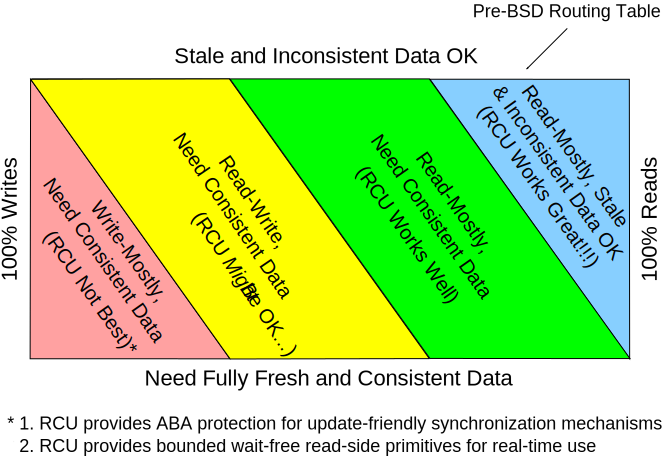
\includegraphics{defer/RCUApplicability}}
\caption{RCU Areas of Applicability}
\label{fig:defer:RCU Areas of Applicability}
\end{figure}

In the meantime,
\cref{fig:defer:RCU Areas of Applicability}
shows some rough rules of thumb on where RCU is most helpful.

As shown in the blue box at the top of the figure, RCU works best if
you have read-mostly data where stale and inconsistent
data is permissible (but see below for more information on stale and
inconsistent data).
The canonical example of this case in the Linux kernel is routing tables.
Because it may have taken many seconds or even minutes for the
routing updates to propagate across the Internet, the system
has been sending packets the wrong way for quite some time.
Having some small probability of continuing to send some of them the wrong
way for a few more milliseconds is almost never a problem.

If you have a read-mostly workload where consistent data is required,
RCU works well, as shown by the green ``read-mostly, need consistent data''
box.
One example of this case is the Linux kernel's mapping from user-level
System-V semaphore IDs to the corresponding in-kernel data structures.
Semaphores tend to be used far more frequently than they are created
and destroyed, so this mapping is read-mostly.
However, it would be erroneous to perform a semaphore operation on
a semaphore that has already been deleted.
This need for consistency is handled by using the lock in the
in-kernel semaphore data structure, along with a ``deleted''
flag that is set when deleting a semaphore.
If a user ID maps to an in-kernel data structure with the
``deleted'' flag set, the data structure is ignored, so that
the user ID is flagged as invalid.

Although this requires that the readers acquire a lock for the
data structure representing the semaphore itself,
it allows them to dispense with locking for the
mapping data structure.
The readers therefore locklessly
traverse the tree used to map from ID to data structure,
which in turn greatly improves performance, scalability, and
real-time response.

As indicated by the yellow ``read-write'' box, RCU can also be useful
for read-write
workloads where consistent data is required, although usually in
conjunction with a number of other synchronization primitives.
For example, the directory-entry cache in recent Linux kernels uses RCU in
conjunction with sequence locks, per-CPU locks, and per-data-structure
locks to allow lockless traversal of pathnames in the common case.
Although RCU can be very beneficial in this read-write case, such
use is often more complex than that of the read-mostly cases.

Finally, as indicated by the red box at the bottom of the figure,
update-mostly workloads requiring
consistent data are rarely good places to use RCU, though there are some
exceptions~\cite{MathieuDesnoyers2012URCU}.
In addition, as noted in
\cref{sec:defer:RCU Provides Type-Safe Memory},
within the Linux kernel, the \co{SLAB_TYPESAFE_BY_RCU}
slab-allocator flag provides type-safe memory to RCU readers, which can
greatly simplify \IXacrl{nbs} and other lockless
algorithms.

In short, RCU is an API that includes a publish-subscribe mechanism for
adding new data, a way of waiting for pre-existing RCU readers to finish,
and a discipline of maintaining multiple versions to allow updates to
avoid harming or unduly delaying concurrent RCU readers.
This RCU API is best suited for read-mostly situations, especially if
stale and inconsistent data can be tolerated by the application.

% defer/rcurelated.tex
% mainfile: ../perfbook.tex
% SPDX-License-Identifier: CC-BY-SA-3.0

\subsection{RCU Related Work}
\label{sec:defer:RCU Related Work}
\OriginallyPublished{Section}{sec:defer:RCU Related Work}{RCU Related Work}{Linux Weekly News}{PaulEMcKenney2014ReadMostly}
\OriginallyPublished{Section}{sec:defer:RCU Related Work}{RCU Related Work}{Linux Weekly News}{PaulEMcKenney2015ReadMostly}

The known first mention of anything resembling RCU took the form of a bug
report from
\ppl{Donald}{Knuth}~\cite[page 413 of Fundamental Algorithms]{Knuth73}
against \ppl{Joseph}{Weizenbaum}'s SLIP list-processing facility for
FORTRAN~\cite{Weizenbaum:1963:SLP:367593.367617}.
Knuth was justified in reporting the bug, as SLIP had no notion of
any sort of grace-period guarantee.

The first known non-bug-report mention of anything resembling RCU appeared
in \pplsur{H. T.}{Kung}'s and \pplsur{Philip L.}{Lehman}'s landmark
paper~\cite{Kung80}.
There was some additional use of this technique in
academia~\cite{Manber82,Manber84,BarbaraLiskov1988ArgusCACM,Pugh90,Andrews91textbook,Pu95a,Cowan96a,Rastogi:1997:LPV:645923.671017,Gamsa99},
but much of the work in this area was carried out by
practitioners~\cite{RichardRashid87a,Hennessy89,Jacobson93,AjuJohn95,Slingwine95,Slingwine97,Slingwine98,McKenney98}.
By the year 2000, the initiative had passed to open-source projects,
most notably the Linux kernel
community~\cite{RustyRussell2000a,RustyRussell2000b,McKenney01b,McKenney01a,McKenney02a,Arcangeli03}.\footnote{
	A list of citations with well over 200 entries may be found in
	\co{bib/RCU.bib} in the {\LaTeX} source for this book.}
RCU was accepted into the Linux kernel in late 2002, with many subsequent
improvements for scalability, robustness, real-time response, energy
efficiency, and specialized use cases.
As of 2021, Linux-kernel RCU is still under active development.

However, in the mid 2010s, there was a welcome upsurge in RCU research
and development across a number of communities and
institutions~\cite{FransKaashoek2015ParallelOSHistory}.
\Cref{sec:defer:RCU Uses} describes uses of RCU,
\cref{sec:defer:RCU Implementations} describes RCU implementations
(as well as work that both creates and uses an implementation),
and finally,
\cref{sec:defer:RCU Validation} describes verification and validation
of RCU and its uses.

\subsubsection{RCU Uses}
\label{sec:defer:RCU Uses}

\ppl{Phil}{Howard} and \ppl{Jon}{Walpole} of Portland State University
(PSU) have
applied RCU to red-black
trees~\cite{PhilHowardPhD,PhilHoward2011RCUTMRBTree} combined with updates
synchronized using software transactional memory.
\ppl{Josh}{Triplett} and \ppl{Jon}{Walpole} (again of PSU)
applied RCU to resizable
hash tables~\cite{JoshTriplettPhD,Triplett:2011:RPHash,JonCorbet2014RCUhash1,JonCorbet2014RCUhash2}.
Other RCU-protected resizable hash tables have been created by
\ppl{Herbert}{Xu}~\cite{HerbertXu2010RCUResizeHash} and by
\ppl{Mathieu}{Desnoyers}~\cite{PaulMcKenney2013LWNURCUhash}.

\ppl{Austin}{Clements}, \ppl{Frans}{Kaashoek}, and \ppl{Nickolai}{Zeldovich}
of MIT created an RCU-optimized balanced binary tree
(Bonsai)~\cite{AustinClements2012RCULinux:mmapsem}, and applied this
tree to the Linux kernel's VM subsystem in order to reduce read-side
contention on the Linux kernel's \co{mmap_sem}.
This work resulted in order-of-magnitude speedups and scalability up to
at least 80 CPUs for a microbenchmark featuring large numbers of minor
page faults.
This is similar to a patch developed earlier by
\ppl{Peter}{Zijlstra}~\cite{PeterZijlstra2014SpeculativePageFault}, and both
were limited by the fact that, at the time, filesystem data structures
were not safe for RCU readers.
\pplsur{Austin}{Clements} et al.\ avoided this limitation by
optimizing the page-fault
path for anonymous pages only.
More recently, filesystem data structures have been made safe for RCU
readers~\cite{JonathanCorbet2010dcacheRCU,JonathanCorbet2011dcacheRCUbug},
so perhaps this work can be implemented for all page types, not just
anonymous pages---\ppl{Peter}{Zijlstra} has, in fact, recently prototyped
exactly this, and \ppl{Laurent}{Dufour} has continued work along these lines.

\ppl{Yandong}{Mao} and \ppl{Robert}{Morris} of MIT and \ppl{Eddie}{Kohler} of
Harvard University created another RCU-protected tree named
Masstree~\cite{Mao:2012:CCF:2168836.2168855} that combines ideas from B+
trees and tries.
Although this tree is about 2.5x slower than an RCU-protected hash table,
it supports operations on key ranges, unlike hash tables.
In addition, Masstree supports efficient storage of objects with long
shared key prefixes and, furthermore, provides persistence via logging
to mass storage.

The paper notes that Masstree's performance rivals that of memcached, even
given that Masstree is persistently storing updates and memcached is not.
The paper also compares Masstree's performance to the persistent
datastores MongoDB, VoltDB, and Redis, reporting significant performance
advantages for Masstree, in some cases exceeding two orders of magnitude.
Another paper~\cite{Tu:2013:STM:2517349.2522713}, by \ppl{Stephen}{Tu},
\ppl{Wenting}{Zheng}, \ppl{Barbara}{Liskov}, and \ppl{Samuel}{Madden}
of MIT and \pplsur{Eddie}{Kohler},
applies Masstree to an in-memory database named Silo, achieving 700K
transactions per second (42M transactions per minute) on a well-known
transaction-processing benchmark.
Interestingly enough, Silo guarantees linearizability without incurring
the overhead of grace periods while holding locks.

\ppl{Maya}{Arbel} and \ppl{Hagit}{Attiya} of Technion took a more rigorous
approach~\cite{MayaArbel2014RCUtree} to an RCU-protected search tree that,
like Masstree, allows concurrent updates.
This paper includes a proof of correctness, including proof that all
operations on this tree are \IX{linearizable}.
Unfortunately, this implementation achieves linearizability by incurring
the full latency of grace-period waits while holding locks, which degrades
scalability of update-only workloads.
One way around this problem is to abandon
linearizability~\cite{AndreasHaas2012FIFOisnt,PaulEMcKennneyAtomicTreeN4037}),
however, Arbel and Attiya instead created an RCU variant that reduces
low-end grace-period latency.
Of course, nothing comes for free, and this RCU variant appears to hit
a scalability limit at about 32 CPUs.
Although there is much to be said for dropping linearizability, thus
gaining both performance and scalability, it is very good to see academics
experimenting with alternative RCU implementations.

\subsubsection{RCU Implementations}
\label{sec:defer:RCU Implementations}

\ppl{Keir}{Fraser} created a user-space RCU named \acr{ebr} for use in
non-blocking synchronization and software transactional
memory~\cite{KeirAnthonyFraserPhD,UCAM-CL-TR-579,KeirFraser2007withoutLocks}.
Interestingly enough, this work cites Linux-kernel RCU on the one hand,
but also inspired the name \acr{qsbr} for the original non-preemptible
Linux-kernel RCU implementation.

\ppl{Mathieu}{Desnoyers} created a user-space RCU for use in
tracing~\cite{MathieuDesnoyers2009URCU,MathieuDesnoyersPhD,MathieuDesnoyers2012URCU},
which has seen use in a number of projects~\cite{MikeDay2013RCUqemu}.

Researchers at Charles University in Prague have also been
working on RCU implementations, including dissertations by
\ppl{Andrej}{Podzimek}~\cite{AndrejPodzimek2010masters} and
\ppl{Adam}{Hraska}~\cite{AdamHraska2013RCUHelenOS}.

\ppl{Yujie}{Liu} (Lehigh University), \ppl{Victor}{Luchangco} (Oracle Labs), and
\ppl{Michael}{Spear} (also Lehigh)~\cite{Liu:2013:MSA:2549695.2549732}
pressed scalable non-zero indicators
(SNZI)~\cite{FaithEllen:2007:SNZI} into service as a grace-period
mechanism.
The intended use is to implement software transactional memory
(see \cref{sec:future:Transactional Memory}), which
imposes linearizability requirements, which in turn seems to
limit scalability.

RCU-like mechanisms are also finding their way into Java.
\pplsur{KC}{Sivaramakrishnan} et al.~\cite{Sivaramakrishnan:2012:ERB:2258996.2259005}
use an RCU-like mechanism to eliminate the read barriers that are
otherwise required when interacting with Java's garbage collector,
resulting in significant performance improvements.

\ppl{Ran}{Liu}, \ppl{Heng}{Zhang}, and \ppl{Haibo}{Chen} of
Shanghai Jiao Tong University
created a specialized variant of RCU that they used for an optimized
``passive reader-writer lock''~\cite{RanLiu2014PassiveRWLock}, similar to
those created by \ppl{Gautham}{Shenoy}~\cite{GauthamShenoy2006RCUrwlock} and
\ppl{Srivatsa}{Bhat}~\cite{SrivatsaSBhat2014RCUrwlock}.
The Liu et al.\ paper is interesting from a number of
perspectives~\cite{PaulEMcKenney2014ReadMostly}.

\ppl{Mike}{Ash} posted~\cite{MikeAsh2015Apple} a description of an RCU-like
primitive in Apple's Objective-C runtime.
This approach identifies read-side critical sections via designated
code ranges, thus qualifying as another method of achieving
zero read-side overhead, albeit one that poses some interesting
practical challenges for large read-side critical sections that
span multiple functions.

\ppl{Pedro}{Ramalhete} and \ppl{Andreia}{Correia}~\cite{PedroRmalhete2015PoorMansRCU}
produced ``Poor Man's RCU'', which, despite using a pair of
\IXhpl{reader-writer}{lock}, manages to provide \IXalt{lock-free}{lock free}
\IXpl{forward-progress guarantee} to
readers~\cite{PaulEMcKenney2015ReadMostly}.

\ppl{Maya}{Arbel} and \ppl{Adam}{Morrison}~\cite{Arbel:2015:PRR:2858788.2688518}
produced ``Predicate RCU'', which works hard to reduce grace-period
duration in order to efficiently support algorithms that hold
update-side locks across grace periods.
This results in reduced batching of updates into grace periods
and reduced scalability, but does succeed in providing short
grace periods.

\QuickQuiz{
	Why not just drop the lock before waiting for the grace
	period, or using something like \co{call_rcu()}
	instead of waiting for a grace period?
}\QuickQuizAnswer{
	The authors wished to support \IX{linearizable} tree
	operations, so that concurrent additions to, deletions
	from, and searches of the tree would appear to execute
	in some globally agreed-upon order.
	In their search trees, this requires holding locks
	across grace periods.
	(It is probably better to drop linearizability as a
	requirement in most cases, but linearizability is a
	surprisingly popular (and costly!) requirement.)
}\QuickQuizEnd

\ppl{Alexander}{Matveev} (MIT), \ppl{Nir}{Shavit} (MIT and Tel-Aviv University),
\ppl{Pascal}{Felber} (University of Neuch\^{a}tel), and \ppl{Patrick}{Marlier} (also
University of Neuch\^{a}tel)~\cite{Matveev:2015:RLS:2815400.2815406}
produced an RCU-like mechanism that can be thought of as
software transactional memory that explicitly marks
read-only transactions.
Their use cases require holding locks across grace periods, which limits
scalability~\cite{PaulEMcKenney2015ReadMostly,PaulEMcKenney2015ReadMostlySidebar}.
This appears to be the first academic RCU-related work to
make good use of the \co{rcutorture} test suite, and also the
first to have submitted a performance improvement to Linux-kernel
RCU, which was accepted into v4.4.

\ppl{Alexander}{Matveev}'s RLU was followed up by MV-RLU from
\ppl{Jaeho}{Kim} et al.~\cite{Kim:2019:MSR:3297858.3304040}.
This work improves scalability over RLU by permitting multiple concurrent
updates, by avoiding holding locks across grace periods, and by using
asynchronous grace periods, for example, \co{call_rcu()} instead of
\co{synchronize_rcu()}.
This paper also made some interesting performance-evaluation choices that
are discussed further in
\cref{sec:future:Deferred Reclamation}
on
\cpageref{sec:future:Deferred Reclamation}.

\ppl{Adam}{Belay} et al.~created an RCU implementation that guards the
data structures used by TCP/IP's address-resolution protocol (ARP)
in their IX operating system~\cite{Belay:2016:IOS:3014162.2997641}.

\ppl{Geoff}{Romer} and \ppl{Andrew}{Hunter} (both at Google) proposed
a cell-based API for RCU
protection of singleton data structures for inclusion in the
C++ standard~\cite{GeoffRomer2018C++DeferredReclamationP0561R4}.

\ppl{Dimitrios}{Siakavaras} et al.~have applied
HTM and RCU to search trees~\cite{Siakavaras2017CombiningHA,DimitriosSiakavaras2020RCU-HTM-B+Trees},
\ppl{Christina}{Giannoula} et al.~have used HTM and RCU to color
graphs~\cite{ChristinaGiannoula2018HTM-RCU-graphcoloring},
and
\ppl{SeongJae}{Park} et al.~have used HTM and RCU to optimize high-contention
locking on \IXacr{numa} systems.

\ppl{Alex}{Kogan} et al.~applied RCU to the construction of range locking
for scalable address spaces~\cite{AlexKogan2020RCUrangelocks}.

\subsubsection{RCU Validation}
\label{sec:defer:RCU Validation}

In early 2017, it is commonly recognized that almost any bug is a potential
security exploit, so validation and verification are first-class concerns.

Researchers at Stony Brook University have produced an RCU-aware data-race
detector~\cite{AbhinavDuggal2010Masters,JustinSeyster2012PhD,Seyster:2011:RFA:2075416.2075425}.
\ppl{Alexey}{Gotsman} of IMDEA, \ppl{Noam}{Rinetzky} of Tel Aviv University,
and \ppl{Hongseok}{Yang} of the University of Oxford have published a
paper~\cite{AlexeyGotsman2012VerifyGraceExtended} expressing the formal
semantics of RCU in terms of separation logic, and have continued with
other aspects of concurrency.

\ppl{Joseph}{Tassarotti} (Carnegie-Mellon University), \ppl{Derek}{Dreyer} (Max
Planck Institute for Software Systems), and \ppl{Viktor}{Vafeiadis}
(also MPI-SWS)~\cite{JosephTassarotti2015RCUproof}
produced a manual formal proof of correctness of the \IXacrf{qsbr} variant of userspace
RCU~\cite{MathieuDesnoyers2009URCU,MathieuDesnoyers2012URCU}.
\ppl{Lihao}{Liang} (University of Oxford), \pplmdl{Paul E.}{McKenney} (IBM),
\ppl{Daniel}{Kroening}, and \ppl{Tom}{Melham}
(both also Oxford)~\cite{LihaoLiang2016VerifyTreeRCU}
used the \IXacrf{cbmc}~\cite{EdmundClarke2004CBMC}
to produce a mechanical proof of correctness of a significant portion
of Linux-kernel Tree RCU\@.
\ppl{Lance}{Roy}~\cite{LanceRoy2017CBMC-SRCU} used CBMC to produce a similar
proof of correctness for a significant portion of Linux-kernel
sleepable RCU (SRCU)~\cite{PaulEMcKenney2006c}.
Finally, \ppl{Michalis}{Kokologiannakis} and \ppl{Konstantinos}{Sagonas}
(National Technical University of
Athens)~\cite{MichalisKokologiannakis2017NidhuggRCU,MichalisKokologiannakis2019RCUstatelessModelCheck}
used the Nighugg tool~\cite{CarlLeonardsson2014Nidhugg}
to produce a mechanical proof of correctness of a somewhat larger
portion of Linux-kernel Tree RCU\@.

None of these efforts located any bugs other than bugs injected into
RCU specifically to test the verification tools.
In contrast,
\ppl{Alex}{Groce} (Oregon State University), \ppl{Iftekhar}{Ahmed},
\ppl{Carlos}{Jensen} (both also OSU), and \pplmdl{Paul E.}{McKenney}
(IBM)~\cite{Groce:2015:VMC:2916135.2916190}
automatically mutated Linux-kernel RCU's source code to test the
coverage of the \co{rcutorture} test suite.
The effort found several holes in this suite's coverage, one of which
was hiding a real bug (since fixed) in Tiny RCU\@.

With some luck, all of this validation work will eventually result in
more and better tools for validating concurrent code.


% defer/rcuexercises.tex
% mainfile: ../perfbook.tex
% SPDX-License-Identifier: CC-BY-SA-3.0

\subsection{RCU Exercises}
\label{sec:defer:RCU Exercises}

This section is organized as a series of Quick Quizzes that invite you
to apply RCU to a number of examples earlier in this book.
The answer to each Quick Quiz gives some hints, and also contains a
pointer to a later section where the solution is explained at length.
The \co{rcu_read_lock()}, \co{rcu_read_unlock()}, \co{rcu_dereference()},
\co{rcu_assign_pointer()}, and \co{synchronize_rcu()} primitives should
suffice for most of these exercises.

\EQuickQuiz{
	The statistical-counter implementation shown in
	\cref{lst:count:Per-Thread Statistical Counters}
	(\path{count_end.c})
	used a global lock to guard the summation in \co{read_count()},
	which resulted in poor performance and negative scalability.
	How could you use RCU to provide \co{read_count()} with
	excellent performance and good scalability.
	(Keep in mind that \co{read_count()}'s scalability will
	necessarily be limited by its need to scan all threads'
	counters.)
}\EQuickQuizAnswer{
	Hint: place the global variable \co{finalcount} and the
	array \co{counterp[]} into a single RCU-protected struct.
	At initialization time, this structure would be allocated
	and set to all zero and \co{NULL}.

	The \co{inc_count()} function would be unchanged.

	The \co{read_count()} function would use \co{rcu_read_lock()}
	instead of acquiring \co{final_mutex}, and would need to
	use \co{rcu_dereference()} to acquire a reference to the
	current structure.

	The \co{count_register_thread()} function would set the
	array element corresponding to the newly created thread
	to reference that thread's per-thread \co{counter} variable.

	The \co{count_unregister_thread()} function would need to
	allocate a new structure, acquire \co{final_mutex},
	copy the old structure to the new one, add the outgoing
	thread's \co{counter} variable to the total, \co{NULL}
	the pointer to this same \co{counter} variable,
	use \co{rcu_assign_pointer()} to install the new structure
	in place of the old one, release \co{final_mutex},
	wait for a grace period, and finally free the old structure.

	Does this really work?
	Why or why not?

	See
	\cref{sec:together:RCU and Per-Thread-Variable-Based Statistical Counters}
	on
	\cpageref{sec:together:RCU and Per-Thread-Variable-Based Statistical Counters}
	for more details.
}\EQuickQuizEnd

\EQuickQuiz{
	\Cref{sec:count:Applying Exact Limit Counters}
	showed a fanciful pair of code fragments that dealt with counting
	I/O accesses to removable devices.
	These code fragments suffered from high overhead on the fastpath
	(starting an I/O) due to the need to acquire a reader-writer
	lock.
	How would you use RCU to provide excellent performance and
	scalability?
	(Keep in mind that the performance of the common-case first
	code fragment that does I/O accesses is much more important
	than that of the device-removal code fragment.)
}\EQuickQuizAnswer{
	Hint: replace the read-acquisitions of the reader-writer lock
	with RCU read-side critical sections, then adjust the
	device-removal code fragment to suit.

	See
	\cref{sec:together:RCU and Counters for Removable I/O Devices}
	on
	\cpageref{sec:together:RCU and Counters for Removable I/O Devices}
	for one solution to this problem.
}\EQuickQuizEnd

% defer/whichtochoose.tex
% mainfile: ../perfbook.tex
% SPDX-License-Identifier: CC-BY-SA-3.0

\section{Which to Choose?}
\label{sec:defer:Which to Choose?}
%
\epigraph{Choose always the way that seems the best, however rough it
	  may be; custom will soon render it easy and agreeable.}
	  {\emph{Pythagoras}}

Section~\ref{sec:defer:Which to Choose? (Overview)}
provides a high-level overview and then
Section~\ref{sec:defer:Which to Choose? (Details)}
provides a more detailed view
of the differences between the deferred-processing techniques presented
in this chapter.
This discussion assumes a linked data structure that is large enough
that readers do not hold references from one traversal to another,
and where elements might be added to and removed from the structure
at any location and at any time.
Section~\ref{sec:defer:Which to Choose? (Production Use)}
then points out a few publicly visible production uses of
hazard pointers, sequence locking, and RCU.
This discussion should help you to make an informed choice between
these techniques.

\subsection{Which to Choose? (Overview)}
\label{sec:defer:Which to Choose? (Overview)}

\begin{table*}
\rowcolors{1}{}{lightgray}
\renewcommand*{\arraystretch}{1.25}
\footnotesize
\centering\OneColumnHSpace{-.3in}
\begin{tabularx}{5.3in}{>{\raggedright\arraybackslash}p{1.1in}
    >{\raggedright\arraybackslash}p{1.0in}
    >{\raggedright\arraybackslash}X
    >{\raggedright\arraybackslash}X
    >{\raggedright\arraybackslash}p{.9in}}
	\toprule
	Property
		& Reference Counting
			& Hazard Pointers
				& Sequence Locks
					& RCU \\
%		  RC	  HP	  SL	  RCU \\
	\midrule
	Readers
		& Slow and unscalable
			& Fast and scalable
				& Fast and scalable
					& Fast and scalable \\
	Number of Protected Objects
		& Scalable
			& Unscalable
				& No protection
					& Scalable \\
	Duration of Protection
		& Can be long
			& Can be long
				& No protection
					& User must bound duration \\
	Need for Traversal Retries
		& If race with object deletion
			& If race with object deletion
				& If race with any update
					& Never \\
	\bottomrule
\end{tabularx}
\caption{Which Deferred Technique to Choose? (Overview)}
\label{tab:defer:Which Deferred Technique to Choose? (Overview)}
\end{table*}

Table~\ref{tab:defer:Which Deferred Technique to Choose? (Overview)}
shows a few high-level properties that distinguish the deferred-reclamation
techniques from one another.

The ``Readers'' row summarizes the results presented in
Figure~\ref{fig:defer:Pre-BSD Routing Table Protected by RCU QSBR},
which shows that all but reference counting are enjoy reasonably
fast and scalable readers.

The ``Number of Protected Objects'' row evaluates each technique's need
for external storage with which to record reader protection.
RCU relies on quiescent states, and thus needs no storage to represent
readers, whether within or outside of the object.
Reference counting can use a single integer within each object in the
structure, and no additional storage is required.
Hazard pointers require external-to-object pointers be provisioned,
and that there be sufficient pointers to handle the maximum number of
objects that a given CPU or thread might need to reference simultaneously.
Of course, sequence locks provides no pointer-traversal protection,
which is why it is normally used on static data.

\QuickQuiz{
	Why can't users dynamically allocate the hazard pointers as they
	are needed?
}\QuickQuizAnswer{
	They can, but at the expense of additional reader-traversal
	overhead and, in some environments, the need to handle
	memory-allocation failure.
}\QuickQuizEnd

The ``Duration of Protection'' describes constraints (if any) on how
long a period of time a user may protect a given object.
Reference counting and hazard pointers can both protect objects for
extended time periods with no untoward side effects, but
maintaining an RCU reference to even one object prevents all other RCU
from being freed.
RCU readers must therefore be relatively short in order to avoid running
the system out of memory, which special-purpose implementations such
as SRCU, Tasks RCU, and Tasks Trace RCU being exceptions to this rule.
Again, sequence locks provide no pointer-traversal protection,
which is why it is normally used on static data.

The ``Need for Traversal Retries'' row tells whether a new reference to
a given object may be acquired unconditionally, as it can with RCU, or
whether the reference acquisition can fail, resulting in a retry
operation, which is the case for reference counting, hazard pointers,
and sequence locks.
In the case of reference counting and hazard pointers, retries are only
required if an attempt to acquire a reference to a given object while
that object is in the process of being deleted, a topic covered in more
detail in the next section.
Sequence locking must of course retry its critical section should it
run concurrently with any update.

\QuickQuiz{
	But don't Linux-kernel \co{kref} reference counters allow
	guaranteed unconditional reference acquisition?
}\QuickQuizAnswer{
	Yes they do, but the guarantee only applies unconditionally
	in cases where a reference is already held.
	With this in mind, please review the paragraph at the beginning of
	Section~\ref{sec:defer:Which to Choose?}, especially the part
	saying ``large enough that readers do not hold references from
	one traversal to another''.
}\QuickQuizEnd

Of course, different rows will have different levels of importance in
different situations.
For example, if your current code is having read-side scalability problems
with hazard pointers, then it does not matter that hazard pointers can require
retrying reference acquisition because your current code already handles
this.
Similarly, if response-time considerations already limit the duration
of reader traversals, as is often the case in kernels and low-level
applications, then it does not matter that RCU has duration-limit
requirements because your code already meets them.
In the same vein, if readers must already write to the objects that they
are traversing, the read-side overhead of reference counters might
not be so important.
Finally, if the data to be protected is in statically allocated variables,
then sequence locking's inability to protect pointers is irrelevant.

Nevertheless, this table should be of great help when choosing between
these techniques.
But those wishing more detail should continue on to the next section.

\subsection{Which to Choose? (Details)}
\label{sec:defer:Which to Choose? (Details)}

\begin{table*}
\rowcolors{1}{}{lightgray}
\renewcommand*{\arraystretch}{1.25}
\footnotesize
\centering\OneColumnHSpace{-.3in}
\begin{tabularx}{5.3in}{>{\raggedright\arraybackslash}p{1.1in}
    >{\raggedright\arraybackslash}p{1.2in}
    >{\raggedright\arraybackslash}X
    >{\raggedright\arraybackslash}X
    >{\raggedright\arraybackslash}p{.9in}}
	\toprule
	Property
		& Reference Counting
			& Hazard Pointers
				& Sequence Locks
					& RCU \\
%		  RC	  HP	  SL	  RCU \\
	\midrule
	Existence Guarantees
		& Complex
			& Yes
				& No
					& Yes \\
	Updates and Readers Progress Concurrently
		& Yes
			& Yes
				& No
					& Yes \\
	Contention Among Readers
		& High
			& None
				& None
					& None \\
	Reader Per\-/Critical\-/Section Overhead
		& N/A
			& N/A
				& Two \tco{smp_mb()}
					& Ranges from none to two
					  \tco{smp_mb()} \\
	Reader Per-Object Traversal Overhead
		& Read-modify-write atomic operations, memory\-/barrier
		  instructions, and cache misses
			& \tco{smp_mb()}
				& None, but unsafe
					& None (volatile accesses) \\
	Reader Forward Progress Guarantee
		& Lock free
			& Lock free
				& Blocking
					& Bounded wait free \\
	Reader Reference Acquisition
		& Can fail (conditional)
			& Can fail (conditional)
				& Unsafe
					& Cannot fail (unconditional) \\
	Memory Footprint
		& Bounded
			& Bounded
				& Bounded
					& Unbounded \\
	Reclamation Forward Progress
		& Lock free
			& Lock free
				& N/A
					& Blocking \\
	Automatic Reclamation
		& Yes
			& Use Case
				& N/A
					& Use Case \\
	Lines of Code
		& 94
			& 79
				& 79
					& 73 \\
	\bottomrule
\end{tabularx}
\caption{Which Deferred Technique to Choose?  (Details)}
\label{tab:defer:Which Deferred Technique to Choose?  (Details)}
\end{table*}

Table~\ref{tab:defer:Which Deferred Technique to Choose? (Details)}
provides more-detailed rules of thumb that can help you choose among the
four deferred-processing techniques presented in this chapter.

As shown in the ``Existence Guarantee'' row,
if you need existence guarantees for linked
data elements, you must use reference counting, hazard pointers, or RCU.
Sequence locks do not provide existence guarantees, instead providing
detection of updates, retrying any read-side critical sections
that do encounter an update.

Of course, as shown in the ``Updates and Readers Progress Concurrently''
row, this detection of updates implies
that sequence locking does not permit updaters and readers to make forward
progress concurrently.
After all, preventing such forward progress is the whole point of using
sequence locking in the first place!
This situation points the way to using sequence locking in conjunction
with reference counting, hazard pointers, or RCU in order to provide
both existence guarantees and update detection.
In fact, the Linux kernel combines RCU and sequence locking in
this manner during pathname lookup.

The ``Contention Among Readers'', ``Reader Per-Critical-Section Overhead'',
and ``Reader Per-Object Traversal Overhead'' rows give a rough sense of
the read-side overhead of these techniques.
The overhead of reference counting can be quite large, with
contention among readers along with a fully ordered read-modify-write
atomic operation required for each and every object traversed.
Hazard pointers incur the overhead of a memory barrier for each data element
traversed, and sequence locks incur the overhead of a pair of memory barriers
for each attempt to execute the critical section.
The overhead of RCU implementations vary from nothing to that of a pair of
memory barriers for each read-side critical section, thus providing RCU
with the best performance, particularly for read-side critical sections
that traverse many data elements.
Of course, the read-side overhead of all deferred-processing variants can
be reduced by batching, so that each read-side operation covers more data.

\QuickQuiz{
	But didn't the answer to one of the quick quizzes in
	Section~\ref{sec:defer:Hazard Pointers}
	say that pairwise asymmetric barriers could eliminate the
	read-side \co{smp_mb()} from hazard pointers?
}\QuickQuizAnswer{
	Yes, it did.
	However, doing this could be argued to change hazard-pointers
	``Reclamation Forward Progress'' row (discussed later) from
	lock-free to blocking because a CPU spinning with interrupts
	disabled in the kernel would prevent the update-side portion of
	the asymmetric barrier from completing.
	In the Linux kernel, such blocking could in theory be prevented
	by building the kernel with \co{CONFIG_NO_HZ_FULL}, designating
	the relevant CPUs as \co{nohz_full} at boot time, ensuring that
	only one thread was ever runnable on a given CPU at a given
	time, and avoiding ever calling into the kernel.
	Alternatively, you could ensure that the kernel was free of any
	bugs that might cause CPUs to spin with interrupts disabled.

	Given that CPUs spinning in the Linux kernel with interrupts
	disabled seems to be rather rare, one might counter-argue that
	asymmetric-barrier hazard-pointer updates are non-blocking
	in practice, if not in theory.
}\QuickQuizEnd

The ``Reader Forward Progress Guarantee'' row shows that only RCU
has a bounded wait-free forward-progress guarantee, which means that
it can carry out a finite traversal by executing a bounded number of
instructions.

The ``Reader Reference Acquisition'' rows indicates that only RCU is
capable of unconditionally acquiring references.
The entry for sequence locks is ``Unsafe'' because, again, sequence locks
detect updates rather than acquiring references.
Reference counting and hazard pointers both require that traversals be
restarted from the beginning if a given acquisition fails.
To see this, consider a linked list containing objects~A, B, C, and~D,
in that order, and the following series of events:

\begin{enumerate}
\item	A reader acquires a reference to object~B.
\item	An updater removes~object B, but refrains from freeing it because
	the reader holds a reference.
	The list now contains objects~A, C, and~D, and
	object~B's \co{->next} pointer is set to \co{HAZPTR_POISON}.
\item	The updater removes object~C, so that the list now contains
	objects~A and~D.
	Because there is no reference to object~C, it is immediately freed.
\item	The reader tries to advance to the successor of the object
	following the now-removed object~B, but the poisoned
	\co{->next} pointer prevents this.
	Which is a good thing, because object~B's \co{->next} pointer
	would otherwise point to the freelist.
\item	The reader must therefore restart its traversal from the head
	of the list.
\end{enumerate}

Thus, when failing to acquire a reference, a hazard-pointer or
reference-counter traversal must restart that traversal from the
beginning.
In the case of nested linked data structures, for example, a
tree containing linked lists, the traversal must be restarted from
the outermost data structure.
This situation gives RCU a significant ease-of-use advantage.

However, RCU's ease-of-use advantage does not come
for free, as can be seen in the ``Memory Footprint'' row.
RCU's support of unconditional reference acquisition means that
it must avoid freeing any object reachable by a given
RCU reader until that reader completes.
RCU therefore has an unbounded memory footprint, at least unless updates
are throttled.
In contrast, reference counting and hazard pointers need to  retain only
those data elements actually referenced by concurrent readers.

This tension between memory footprint and acquisition
failures is sometimes resolved within the Linux kernel by combining use
of RCU and reference counters.
RCU is used for short-lived references, which means that RCU read-side
critical sections can be short.
These short RCU read-side critical sections in turn mean that the corresponding
RCU grace periods can also be short, which limits the memory footprint.
For the few data elements that need longer-lived references, reference
counting is used.
This means that the complexity of reference-acquisition failure only
needs to be dealt with for those few data elements:  The bulk of
the reference acquisitions are unconditional, courtesy of RCU.
See Section~\ref{sec:together:Refurbish Reference Counting}
for more information on combining reference counting with other
synchronization mechanisms.

The ``Reclamation Forward Progress'' row shows that hazard pointers
can provide non-blocking updates~\cite{MagedMichael04a,HerlihyLM02}.
Reference counting might or might not, depending on the implementation.
However, sequence locking cannot provide non-blocking updates, courtesy
of its update-side lock.
RCU updaters must wait on readers, which also rules out fully non-blocking
updates.
However, there are situations in which the only blocking operation is
a wait to free memory, which results in a situation that, for many
purposes, is as good as non-blocking~\cite{MathieuDesnoyers2012URCU}.

As shown in the ``Automatic Reclamation'' row, only reference
counting can automate freeing of memory, and even then only
for non-cyclic data structures.
Certain use cases for hazard pointers and RCU can provide automatic
reclamation using \emph{link counts}, which can be thought of as
reference counts, but applying only to incoming links from other
parts of the data structure~\cite{MagedMichael2018FollyHazptr}.

Finally, the ``Lines of Code'' row shows the size of the Pre-BSD
Routing Table implementations, giving a rough idea of relative ease of use.
That said, it is important to note that the reference-counting and
sequence-locking implementations are buggy, and that a correct
reference-counting implementation is considerably
more complex~\cite{Valois95a,MagedMichael95a}.
For its part, a correct sequence-locking implementation requires
the addition of some other synchronization mechanism, for example,
hazard pointers or RCU, so that sequence locking detects concurrent
updates and the other mechanism provides safe reference acquisition.

As more experience is gained using these techniques, both separately
and in combination, the rules of thumb laid out in this section will
need to be refined.
However, this section does reflect the current state of the art.

\subsection{Which to Choose? (Production Use)}
\label{sec:defer:Which to Choose? (Production Use)}

This section points out a few publicly visible production uses of
hazard pointers, sequence locking, and RCU.
Reference counting is omitted, not because it is unimportant, but rather
because it is not only used pervasively, but heavily documented in textbooks
going back a half century.
One of the hoped-for benefits of listing production uses of these other
techniques is to provide examples to study---or to find bugs in, as
the case may be.\footnote{
	Kudos to Mathias Stearn, Matt Wilson, David Goldblatt, LiveJournal
	user fanf, Nadav Har'El, Avi Kivity, Dmitry Vyukov, Raul Guitterez
	S., Twitter user @peo3, Paolo Bonzini, and Thomas Monjalon for
	locating a great many of these use cases.}

\subsubsection{Production Uses of Hazard Pointers}
\label{sec:defer:Production Uses of Hazard Pointers}

In 2010, Keith Bostic added hazard pointers to
WiredTiger~\cite{KeithBostic2010WiredTigerhazptr}.
MongoDB 3.0, released in 2015, included WiredTiger and thus hazard pointers.

In 2011, Samy Al Bahra added hazard pointers to the Concurrency Kit
library~\cite{SamyAlBahra2011ckhp}.

In 2014, Maxim Khizhinsky added hazard pointers to
libcds~\cite{MaximKhizhinsky2014libcdsHazptr}.

In 2015, David Gwynne introduced shared reference pointers, a form
of hazard pointers, to OpenBSD~\cite{DavidGwynne2015srp}.

In 2017--2018, the Rust-language
\co{arc-swap}~\cite{MichalVaner2018arc-swapHazptr} and
\co{conc}~\cite{crates.io.user.ticki2017concHazptr}
crates rolled their own implementations of hazard pointers.

In 2018, Maged Michael added hazard pointers to Facebook's Folly
library~\cite{MagedMichael2018FollyHazptr}, where it is used heavily.

\subsubsection{Production Uses of Sequence Locking}
\label{sec:defer:Production Uses of Sequence Locking}

The Linux kernel added sequence locking to v2.5.60 in
2003~\cite{JonathanCorbet2003seqlock}, having been generalized from
an ad-hoc technique used in x86's implementation of the
\co{gettimeofday()} system call.

In 2011, Samy Al Bahra added sequence locking to the Concurrency Kit
library~\cite{SamyAlBahra2011ckseqlock}.

Paolo Bonzini added a simple sequence-lock to the QEMU emulator in
2013~\cite{PaoloBonzini2013QEMUseqlock}.

Alexis Menard abstracted a sequence-lock implementation in Chromium
in 2016~\cite{AlexisMenard2016ChromiumSeqLock}.

A simple sequence locking implementation was added to \co{jemalloc()}
in 2018~\cite{DavidGoldblatt2018seqlock}.
The eigen library also has a special-purpose queue that is managed by
a mechanism resembling sequence locking.

\subsubsection{Production Uses of RCU}
\label{sec:defer:Production Uses of RCU}

IBM's VM/XA is adopted passive serialization, a mechanism similar to
RCU, some time in the 1980s~\cite{Hennessy89}.

DYNIX/ptx adopted RCU in 1993~\cite{McKenney98,Slingwine95}.

The Linux kernel adopted Dipankar Sarma's implementation of RCU in
2002~\cite{Torvalds2.5.43}.

The userspace RCU project started in 2009~\cite{MathieuDesnoyers2009URCU}.

The Knot DNS project started using the userspace RCU
library in 2010~\cite{LubosSlovak2010KnotDNSRCU}.
That same year, the OSv kernel added an RCU
implementation~\cite{AviKivity2013OSvRCU},
later adding an RCU-protected linked list~\cite{AviKivity2013OSvRCUlist}
and an RCU-protected hash table~\cite{AviKivity2013OSvRCUhash}.

In 2011, Samy Al Bahra added epochs
(a form of RCU~\cite{UCAM-CL-TR-579,KeirFraser2007withoutLocks})
to the Concurrency Kit
library~\cite{SamyAlBahra2011ckEpoch}.

NetBSD began using the aforementioned passive serialization with v6.0 in
2012~\cite{NetBSD2012pserialize}.
Among other things, passive serialization is used in
NetBSD packet filter (NPF)~\cite{MindaugasRasiukevicius2014NPFRCU}.

Paolo Bonzini added RCU support to the QEMU emulator in 2015 via a
friendly fork of the userspace RCU
library~\cite{MikeDay2013RCUqemu,PaoloBonzini2013QEMURCU}.

In 2015, Maxim Khizhinsky added RCU to
libcds~\cite{MaxKhiszinsky2015C++RCU}.

Mindaugas Rasiukevicius implemented libqsbr in 2016, which features
QSBR and epoch-based reclamation
(EBR)~\cite{MindaugasRasiukevicius2016libqsbr},
both of which are types of implementations of RCU.

Sheth et al.~\cite{HarshalSheth2016goRCU}
demonstrated the value of leveraging Go's garbage
collector to provide RCU-like functionality, and
the Go programming language provides a \co{Value} type that can
provide this functionality.\footnote{
	See \url{https://golang.org/pkg/sync/atomic/\#Value}, particularly
	the ``Example (ReadMostly)''.}

Matt Klein describes an RCU-like mechanism that is used in the Envoy
Proxy~\cite{MattKlein2017EnvoyRCU}.

Honnappa Nagarahalli added an RCU library to the Data Plane Development
Kit (DPDK) in 2018~\cite{HonnappaNagarahalli2018dpdkRCU}.

Stjepan Glavina merged an epoch-based RCU implementation into the
\co{crossbeam} set of concurrency-support ``crates'' for the Rust
language~\cite{StjepanGlavina2018RustRCU}.

Finally, any garbage-collected concurrent language (not just Go!) gets
the update side of an RCU implementation at zero incremental cost.

\subsubsection{Summary of Production Uses}
\label{sec:defer:Summary of Production Uses}

Perhaps the time will come when sequence locking, hazard pointers, and
RCU are all as heavily used and as well known as are reference counters.
Until that time comes, the current production uses of these mechanisms
should help guide the choice of mechanism as well as showing how best
to apply each of them.

The next section discusses updates, a ticklish issue for many of the
read-mostly mechanisms described in this chapter.

% defer/updates.tex
% mainfile: ../perfbook.tex
% SPDX-License-Identifier: CC-BY-SA-3.0

\section{What About Updates?}
\label{sec:defer:What About Updates?}
%
\epigraph{The only thing constant in life is change.}
	 {Fran\c{c}ois de la Rochefoucauld}

The deferred-processing techniques called out in this chapter are most
directly applicable to read-mostly situations, which begs the question
``But what about updates?''
After all, increasing the performance and scalability of readers is all
well and good, but it is only natural to also want great performance and
scalability for writers.

We have already seen one situation featuring high performance and
scalability for writers, namely the counting algorithms surveyed in
Chapter~\ref{chp:Counting}.
These algorithms featured partially partitioned data structures so
that updates can operate locally, while the more-expensive reads
must sum across the entire data structure.
Silas Boyd-Wickhizer has generalized this notion to produce
OpLog, which he has applied to
Linux-kernel pathname lookup, VM reverse mappings, and the \co{stat()} system
call~\cite{SilasBoydWickizerPhD}.

Another approach, called ``Disruptor'', is designed for applications
that process high-volume streams of input data.
The approach is to rely on single-producer-single-consumer FIFO queues,
minimizing the need for synchronization~\cite{AdrianSutton2013LCA:Disruptor}.
For Java applications, Disruptor also has the virtue of minimizing use
of the garbage collector.

And of course, where feasible, fully partitioned or ``sharded'' systems
provide excellent performance and scalability, as noted in
Chapter~\ref{cha:Partitioning and Synchronization Design}.

The next chapter will look at updates in the context of several types
of data structures.


\QuickQuizAnswersChp{qqzdefer}
